\documentclass[twoside]{book}

% Packages required by doxygen
\usepackage{fixltx2e}
\usepackage{calc}
\usepackage{doxygen}
\usepackage{graphicx}
\usepackage[utf8]{inputenc}
\usepackage{makeidx}
\usepackage{multicol}
\usepackage{multirow}
\PassOptionsToPackage{warn}{textcomp}
\usepackage{textcomp}
\usepackage[nointegrals]{wasysym}
\usepackage[table]{xcolor}

% Font selection
\usepackage[T1]{fontenc}
\usepackage{mathptmx}
\usepackage[scaled=.90]{helvet}
\usepackage{courier}
\usepackage{amssymb}
\usepackage{sectsty}
\renewcommand{\familydefault}{\sfdefault}
\allsectionsfont{%
  \fontseries{bc}\selectfont%
  \color{darkgray}%
}
\renewcommand{\DoxyLabelFont}{%
  \fontseries{bc}\selectfont%
  \color{darkgray}%
}
\newcommand{\+}{\discretionary{\mbox{\scriptsize$\hookleftarrow$}}{}{}}

% Page & text layout
\usepackage{geometry}
\geometry{%
  a4paper,%
  top=2.5cm,%
  bottom=2.5cm,%
  left=2.5cm,%
  right=2.5cm%
}
\tolerance=750
\hfuzz=15pt
\hbadness=750
\setlength{\emergencystretch}{15pt}
\setlength{\parindent}{0cm}
\setlength{\parskip}{0.2cm}
\makeatletter
\renewcommand{\paragraph}{%
  \@startsection{paragraph}{4}{0ex}{-1.0ex}{1.0ex}{%
    \normalfont\normalsize\bfseries\SS@parafont%
  }%
}
\renewcommand{\subparagraph}{%
  \@startsection{subparagraph}{5}{0ex}{-1.0ex}{1.0ex}{%
    \normalfont\normalsize\bfseries\SS@subparafont%
  }%
}
\makeatother

% Headers & footers
\usepackage{fancyhdr}
\pagestyle{fancyplain}
\fancyhead[LE]{\fancyplain{}{\bfseries\thepage}}
\fancyhead[CE]{\fancyplain{}{}}
\fancyhead[RE]{\fancyplain{}{\bfseries\leftmark}}
\fancyhead[LO]{\fancyplain{}{\bfseries\rightmark}}
\fancyhead[CO]{\fancyplain{}{}}
\fancyhead[RO]{\fancyplain{}{\bfseries\thepage}}
\fancyfoot[LE]{\fancyplain{}{}}
\fancyfoot[CE]{\fancyplain{}{}}
\fancyfoot[RE]{\fancyplain{}{\bfseries\scriptsize Generated on Mon Jul 14 2014 14\+:02\+:55 for vw4tools by Doxygen }}
\fancyfoot[LO]{\fancyplain{}{\bfseries\scriptsize Generated on Mon Jul 14 2014 14\+:02\+:55 for vw4tools by Doxygen }}
\fancyfoot[CO]{\fancyplain{}{}}
\fancyfoot[RO]{\fancyplain{}{}}
\renewcommand{\footrulewidth}{0.4pt}
\renewcommand{\chaptermark}[1]{%
  \markboth{#1}{}%
}
\renewcommand{\sectionmark}[1]{%
  \markright{\thesection\ #1}%
}

% Indices & bibliography
\usepackage{natbib}
\usepackage[titles]{tocloft}
\setcounter{tocdepth}{3}
\setcounter{secnumdepth}{5}
\makeindex

% Custom commands
\newcommand{\clearemptydoublepage}{%
  \newpage{\pagestyle{empty}\cleardoublepage}%
}


%===== C O N T E N T S =====

\begin{document}

% Titlepage & ToC
\pagenumbering{roman}
\begin{titlepage}
\vspace*{7cm}
\begin{center}%
{\Large vw4tools \\[1ex]\large 0.\+9-\/89 }\\
\vspace*{1cm}
{\large Generated by Doxygen 1.8.7}\\
\vspace*{0.5cm}
{\small Mon Jul 14 2014 14:02:55}\\
\end{center}
\end{titlepage}
\clearemptydoublepage
\tableofcontents
\clearemptydoublepage
\pagenumbering{arabic}

%--- Begin generated contents ---
\chapter{Java\+Doc A\+P\+I Markup for vw4tools}
\label{index}\section*{vw4tools }

Tools and utilities for Virtual\+Wisdom4

At current, V\+W4\+Tools is a script or two, plus one big jar file. vw4tool.\+jar allows a user to import a text file in one of several formats and output an Entity import J\+S\+O\+N for Virtual\+Wisdom4.

\section*{Running Java }

In this document, it is assumed \char`\"{}java\char`\"{} runs from the command prompt. In some cases, this isn't true. Windows users, for example, may need to change their usage, from\+: \begin{DoxyVerb}java -jar vw4tool.jar ...
\end{DoxyVerb}


to\+: \begin{DoxyVerb}java.exe -jar vw4tool.jar ...
\end{DoxyVerb}


In both cases, if the \char`\"{}java\char`\"{} (or java.\+exe) executable is not available on the user's \char`\"{}path\char`\"{} or list of locations wherein to find a binary/executable, the user will need to type the full pathname to the java executable.

Macintosh O\+S\+X users can simply type \char`\"{}java\char`\"{}\+: \begin{DoxyVerb}java -jar vw4tool.jar ...
\end{DoxyVerb}


A U\+N\+I\+X (or unix-\/like) user may need to type /opt/local/bin/java or similar\+: \begin{DoxyVerb}/opt/local/bin/java -jar vw4tool.jar ...
\end{DoxyVerb}


A Windows user may need to type a full pathname such as\+: \begin{DoxyVerb}"C:\Program Files (x86)\Java\jre7\bin\java.exe" -jar vw4tool.jar ...
\end{DoxyVerb}


In all cases, where I type merely \char`\"{}java\char`\"{}, make sure you replace that with however the invocation details are for your platform.

To confirm you've found a working Java Runtime Environment, use the \char`\"{}help\char`\"{} command to as vw4tool.\+jar what version it is\+: \begin{DoxyVerb}java -jar vw4tool.jar --help
Usage: vw4tool -V|--version|-H|--help
     : vw4tool --read <filename>|--input <filename> | -r <filename> | -i <filename>
   ie: vw4tool --read import.json
   ie: vw4tool -r import.json
\end{DoxyVerb}


note\+: many commands have shorter versions. \char`\"{}-\/-\/version\char`\"{} (with two \char`\"{}-\/\char`\"{}) is the same as \char`\"{}-\/\+V\char`\"{} (with one dash). Pay special attention to case. Uppercase \char`\"{}\+N\char`\"{} is different from lowercase \char`\"{}n\char`\"{}.

\section*{Common Usage }

\begin{DoxyVerb}java -jar vw4tool.jar  -N localfile1.txt -N localfile2.txt -N localfile3.txt -oexample.json
\end{DoxyVerb}


or \begin{DoxyVerb}java -jar vw4tool.jar  -N localfile1.txt -N localfile2.txt -N localfile3.txt -oOrderedTuples.csv
awk -f csv-to-json.awk OrderedTuples.csv > example.json
\end{DoxyVerb}


This is the most common usage, here as a reference. Notice that although this shows E\+I\+T\+H\+E\+R Ordered\+Tuples.\+csv or a J\+S\+O\+N file being created, both could be created by multiple \char`\"{}-\/o\char`\"{} options. Notice also that although in past, \char`\"{}-\/o\char`\"{} was \char`\"{}cuddled\char`\"{} to the filename after it (no spaces), but this has changed to make it easier and more forgiving to use.

\section*{Overview }

In general, collection and conversion looks like the following diagram\+:

\begin{center}

\begin{DoxyImageNoCaption}
  \mbox{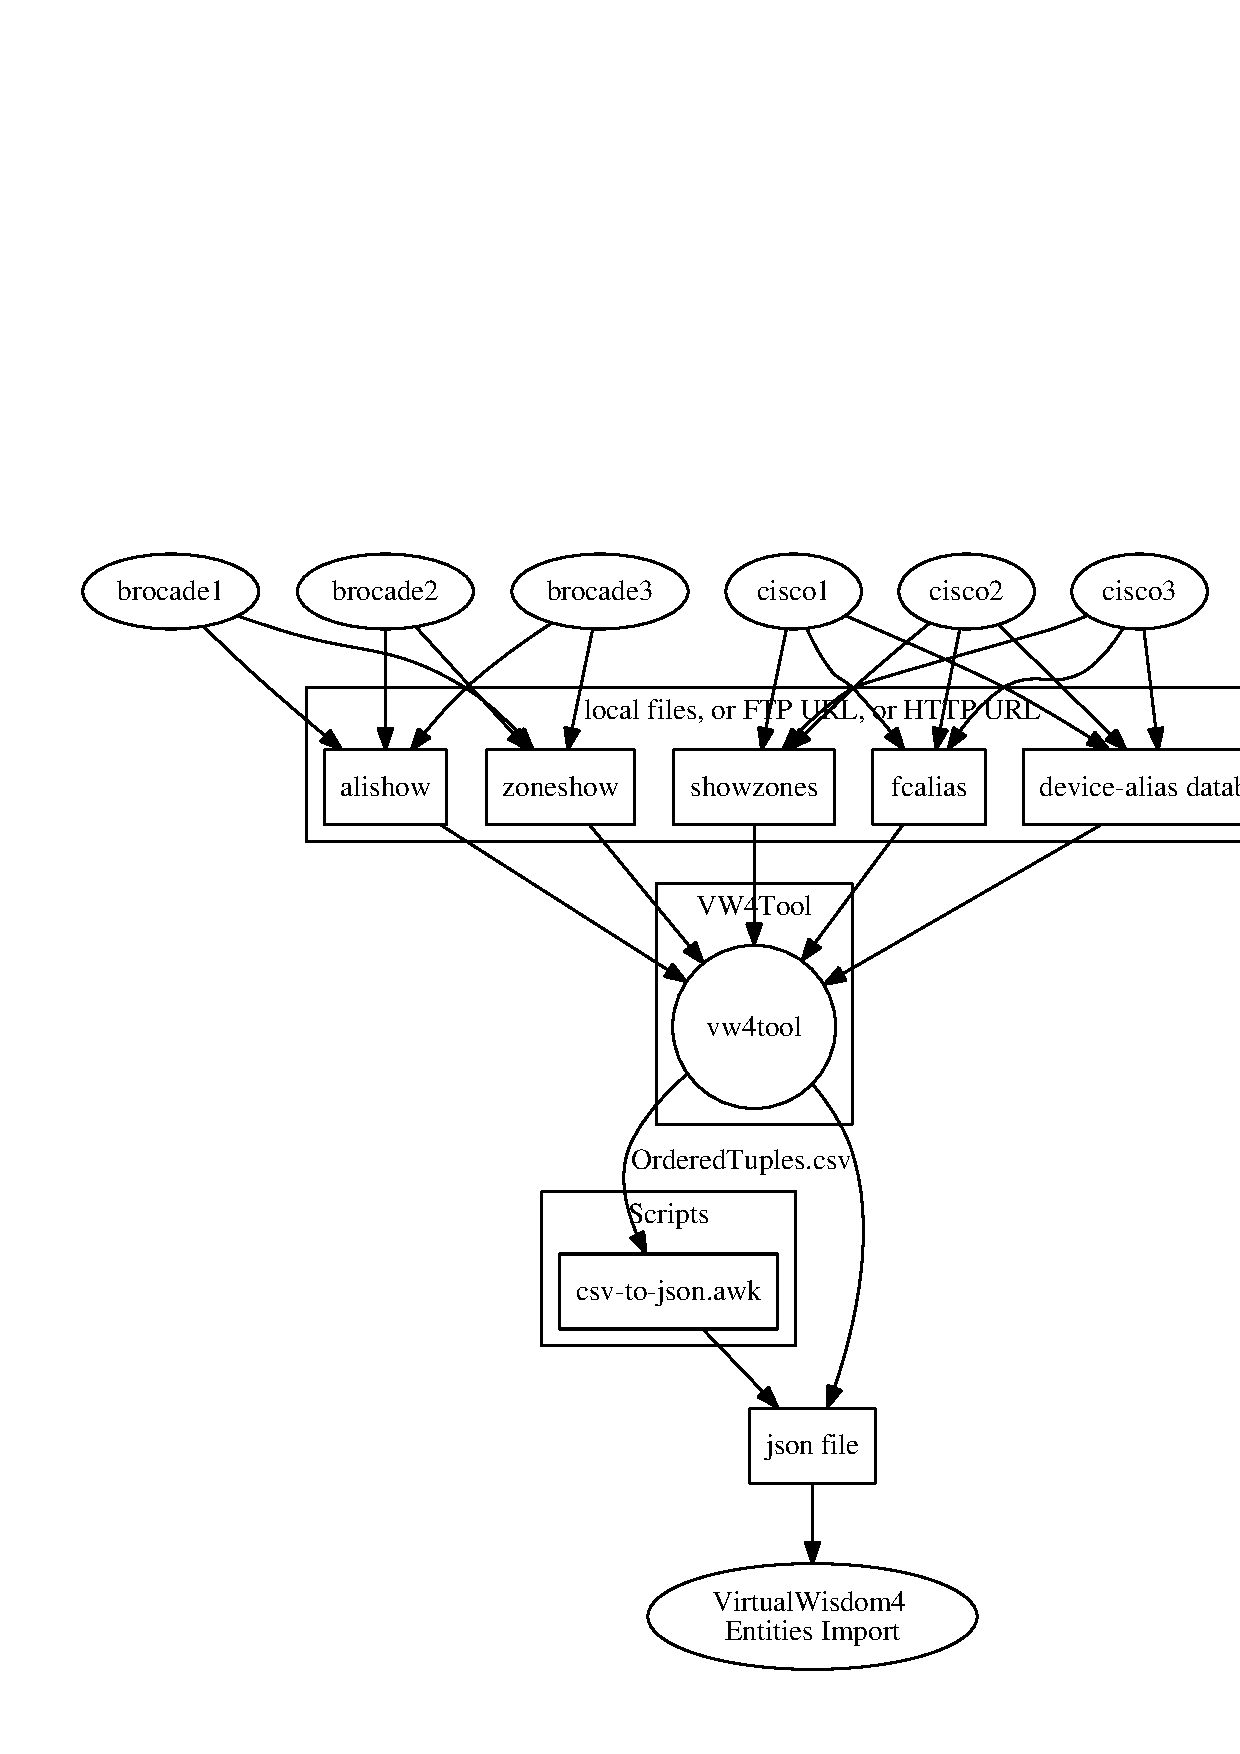
\includegraphics[width=\textwidth,height=\textheight/2,keepaspectratio=true]{dot_inline_dotgraph_1}}
\end{DoxyImageNoCaption}
\end{center}


\section*{Import of F\+T\+P or H\+T\+T\+P Data }

V\+W4\+Tools uses the U\+R\+L\+Data\+Source functionality to open a stream from a H\+T\+T\+P or F\+T\+P server; this means that the files it parses can be stored on a local filesystem, a F\+T\+P server, and an H\+T\+T\+P server as constant data, or can be the result of a C\+G\+I program on an H\+T\+T\+P server. Less common, a local file may also be mounted as a F\+U\+S\+E filesystem, allowing even \char`\"{}local\char`\"{} data to be generated like a C\+G\+I program.

In order to draw a text stream from a F\+T\+P server or H\+T\+T\+P server, merely use a R\+F\+C-\/1738-\/compliant U\+R\+L to indicate these two sources\+: \begin{DoxyVerb}(ftp|http)://{user{:password@@}server{:port}/pathname/to/resource
\end{DoxyVerb}


for example\+:

(basic user/pass\+: user = scott, pass = T1ger, host = ftp.\+example.\+com, subdir = . , file = nicknames.\+txt \begin{DoxyVerb}java -jar vw4tool.jar --nickname=ftp://scott:T1ger@@ftp.example.com/nicknames.txt
\end{DoxyVerb}


(basic user/pass\+: user = scott, pass = T1ger, host = ftp.\+example.\+com, subdir = /users/local/\+Scott\+Adams/ , file = aliases.\+text \begin{DoxyVerb}java -jar vw4tool.jar --nickname=ftp://scott:T1ger@@ftp.example.com/%2fusers/local/ScottAdams/aliases.text
\end{DoxyVerb}


(basic user/pass\+: user = anonymous, pass = scott@uberserver.\+net, host = ftp.\+example.\+com, subdir = examples , file = aliases \begin{DoxyVerb}java -jar vw4tool.jar -N ftp://anonymous:scott%2Fuberserver.net@@ftp.example.com/examples/aliases
\end{DoxyVerb}


(basic http\+: host = www.\+example.\+com, subdir = . , file = aliases \begin{DoxyVerb}java -jar vw4tool.jar --nickname=http://www.example.com/aliases
\end{DoxyVerb}


(basic H\+T\+T\+P G\+E\+T\+: host = www.\+example.\+com, subdir = . , path=/cgi-\/bin/fetch.cgi, some parameters \begin{DoxyVerb}java -jar vw4tool.jar --nickname=http://www.example.com/cgi-bin/fetch.cgi?now=20140901&realm=WEST&group=production
\end{DoxyVerb}


N\+O\+T\+E\+: \char`\"{}-\/-\/nickname=\char`\"{} and \char`\"{}-\/\+N\char`\"{} are functionally identical; \char`\"{}-\/-\/nickname=\char`\"{} may offer a slight beefit in more clearly self-\/documenting the behavior of the commandline option.

\section*{Import of Local Text File }

The most common usage is local text files representing the metadata of the local environment. This is done by offering a R\+F\+C-\/1738-\/compliant local file U\+R\+L\+: \begin{DoxyVerb}file://pathname/to/resource
\end{DoxyVerb}


Note that if the \char`\"{}file\+://\char`\"{} is not given, and no \char`\"{}protocol\char`\"{} (ie \char`\"{}file\+://\char`\"{}) is given, vw4tool will warn you about this but try the local {\tt file\+://} protocol prefix for you

for example\+:

(local file in subdir ./files/aliases) \begin{DoxyVerb}java -jar vw4tool.jar --nickname=file://files/aliases
java -jar vw4tool.jar --nickname=files/aliases
\end{DoxyVerb}


(local file in subdir /\+Full/\+Path/files/aliases) \begin{DoxyVerb}java -jar vw4tool.jar --nickname=file:///Full/Path/files/aliases
java -jar vw4tool.jar --nickname=/Full/Path/files/aliases
\end{DoxyVerb}


\section*{Specifying Formats }

The user doesn't need to speficy the format of a file; vw4tool will try the file at the same time across many different parsers and see which one can make sense of it. Unfortunately, the parsers cannot always chew through any user-\/interface codes (such as \char`\"{}press any key to continue\char`\"{}) and preamble (the verbose text trash before the actual zone or aliases or such). Trimming that to a minimum offers a better chance of parsing the file.

The corollary to this is that if a file doesn't seem to parse, yet it seems like it should, remove anything before or after the actual content, and confirm that it was collected in a non-\/interactive method. If the user ever needs to \char`\"{}press any key for more\char`\"{}, chances are, the parsed result will be either partial, or none at all.

\section*{Multiple Inputs }

These input formats can be mixed. For example \begin{DoxyVerb}java -jar vw4tool.jar --nickname=http://www.example.com/cgi-bin/fetch.cgi?now=20140901&realm=WEST&group=production -N local.txt -N file:///Users/allanc/aliases.dad -N morefiles.txt
\end{DoxyVerb}


\section*{Outputs }

vw4tool will either generate an Ordered\+Tuples.\+csv file (if that specific filename is given on the \char`\"{}-\/o\char`\"{} option) or a json file (any other putput filename). Or both\+: \begin{DoxyVerb}java -jar vw4tool.jar  -N local.txt -oOrderedTuples.csv -oexample.json
\end{DoxyVerb}


N\+O\+T\+E\+: giving no filename used to send the output to stdout, but now requires a \char`\"{}-\/\char`\"{} to mean \char`\"{}yes, I meant that\char`\"{}\+: \begin{DoxyVerb}java -jar vw4tool.jar  -N local.txt -o -
\end{DoxyVerb}


For this reason, the following two commands used to do different things, but are now equivalent\+: \begin{DoxyVerb}java -jar vw4tool.jar  -N local.txt -oexample.json
java -jar vw4tool.jar  -N local.txt -o example.json
\end{DoxyVerb}


\section*{Proprietary Intellectual Property }

With the exception of samples/import01.\+json, all files and content are based on the same level of access to the product enjoyed by a customer. Implicitly, no private information is shared, all of this content (save the one file) is based on empirical discovery, and could change overnight. 
\chapter{R\+E\+A\+D\+M\+E}
\label{md_htdocs_README}
\input{md_htdocs_README}
\chapter{csv-\/to-\/json.awk\+: Convert a \char`\"{}\+Ordered\+Tuples.\+csv\char`\"{} file to a J\+S\+O\+N Entity import}
\label{csv-to-json}
\section{Overview}\label{csv-to-json_Overview}
This script (\doxyref{csv-\/to-\/json.\+awk}{p.}{csv-to-json_8awk}) interprets a basic 4-\/column C\+S\+V into a J\+S\+O\+N entities file. This is \char`\"{}the old method\char`\"{}, but facilitates hand-\/tweaking if required. In essence, the four columns of the file are\+:


\begin{DoxyEnumerate}
\item host/array name
\item device type\+: \char`\"{}host\char`\"{} or \char`\"{}array\char`\"{} (without quotes)
\item W\+W\+P\+N
\item optional unique name of the W\+W\+P\+N within the (column 1) host
\end{DoxyEnumerate}

For example\+:

\begin{TabularC}{4}
\hline
\rowcolor{lightgray}{\bf name }&{\bf type }&\PBS\centering {\bf W\+W\+P\+N }&{\bf (optional) name  }\\\cline{1-4}
M\+P\+V123456-\/001 &host &\PBS\centering 2001001560123456 &M\+P\+V123456-\/001 \\\cline{1-4}
M\+P\+V123456-\/013 &host &\PBS\centering 2013001560123456 &M\+P\+V123456-\/013 \\\cline{1-4}
Net\+App-\/123456 &array &\PBS\centering 500a098598123456 &\\\cline{1-4}
Net\+App-\/123456 &array &\PBS\centering 500a098698123456 &\\\cline{1-4}
Oracle01 &host &\PBS\centering 10\+:00\+:00\+:00\+:c9\+:12\+:34\+:56 &Oracle01-\/\+A \\\cline{1-4}
Oracle01 &host &\PBS\centering 10\+:00\+:00\+:00\+:c9\+:12\+:34\+:57 &Oracle01-\/\+B \\\cline{1-4}
\end{TabularC}
\section{Running this Script}\label{csv-to-json_running}
This A\+W\+K script should work with gawk.\+exe from the Unx\+Utils project on sourceforge.\+net (which offers windows binaries without need of cygwin) and is regression-\/tested using basic awk on B\+S\+D-\/based operating systems. \begin{DoxyVerb}gawk.exe   -f csv-to-json.awk   OrderedTuples.csv   >   customer-name.json
\end{DoxyVerb}
\section{Commandline Variables\+:}\label{csv-to-json_cmdline}

\begin{DoxyItemize}
\item -\/v S\+K\+I\+P\+A\+R\+R\+A\+Y=\{something\} will avoid exporting the array which contains iomodules
\item -\/v S\+K\+I\+P\+H\+O\+S\+T=\{something\} will avoid exporting the host which contains hbas
\end{DoxyItemize}\section{Usage (2 switches)}\label{csv-to-json_Example}
\begin{DoxyVerb}plink.exe -l username -pw pAssw0rd 192.168.1.44 'show device-alias database' > SW44.dad
plink.exe -l username -pw pAssw0rd 192.168.1.42 'zoneshow' > SW42.zoneshow
java.exe   -jar vw4tool.jar   -N SW44.dad   -N SW42.zoneshow   -oOrderedTuples.csv
\end{DoxyVerb}


(manual changes to the Ordered\+Tuples.\+csv file) \begin{DoxyVerb}sort.exe OrderedTuples.csv    | gawk.exe   -f csv-to-json.awk   >  customer-name.json
\end{DoxyVerb}


If the user wants to avoid showing hosts in that output (but still produce H\+B\+As)\+: \begin{DoxyVerb}plink.exe -l username -pw pAssw0rd 192.168.1.44 'show device-alias database' > SW44.dad
plink.exe -l username -pw pAssw0rd 192.168.1.42 'zoneshow' > SW42.zoneshow
java.exe   -jar vw4tool.jar   -N SW44.dad   -N SW42.zoneshow   -oOrderedTuples.csv
sort.exe OrderedTuples.csv    | gawk.exe   -v SKIPHOST=gary.yuen   -f csv-to-json.awk   >  customer-name.json
\end{DoxyVerb}


It is assumed the user wants to make changes to Ordered\+Tuples.\+csv before the final step; otherwise, the last two steps may be combined (which avoids this script)\+: \begin{DoxyVerb}plink.exe -l username -pw pAssw0rd 192.168.1.44 'show device-alias database' > SW44.dad
plink.exe -l username -pw pAssw0rd 192.168.1.42 'zoneshow' > SW42.zoneshow
java.exe   -jar vw4tool.jar   -N SW44.dad   -N SW42.zoneshow   -ocustomer-name.json  \end{DoxyVerb}
 
\chapter{Todo List}
\label{todo}

\begin{DoxyRefList}
\item[\label{todo__todo000001}%
Global \doxyref{Virtual\+Wisdom4\+Client\+Tool.\+\_\+load}{p.}{classorg_1_1smallfoot_1_1vw4_1_1VirtualWisdom4ClientTool_ad9a051ba608e7fcb9adac39bc3946058} (String filename)]\+: evaluate\+: mapper.\+configure(Deserialization\+Config.\+Feature.\+F\+A\+I\+L\+\_\+\+O\+N\+\_\+\+U\+N\+K\+N\+O\+W\+N\+\_\+\+P\+R\+O\+P\+E\+R\+T\+I\+E\+S, false);  
\item[\label{todo__todo000002}%
Global \doxyref{Virtual\+Wisdom4\+Client\+Tool.main}{p.}{classorg_1_1smallfoot_1_1vw4_1_1VirtualWisdom4ClientTool_a75988cf84fc6ee7a2ebff36e363021aa} (String args\mbox{[}\mbox{]})]need to check 3-\/decimal values such as \char`\"{}-\/t 4.\+0.\+1.\+7\char`\"{} (see also testsuite.\+at.\+in) 
\end{DoxyRefList}
\chapter{Commandline Options}
\label{cmdopt}

\begin{DoxyRefList}
\item[\label{cmdopt__cmdopt000001}%
Global \doxyref{Virtual\+Wisdom4\+Client\+Tool.main}{p.}{classorg_1_1smallfoot_1_1vw4_1_1VirtualWisdom4ClientTool_a75988cf84fc6ee7a2ebff36e363021aa} (String args\mbox{[}\mbox{]})]-\/\+H$\vert$--help Show a simple help screen as a reminder of options which are understood by the application 


\begin{DoxyCode}
java -jar vw4tools.jar --help 
\end{DoxyCode}


-\/\+V$\vert$--version Show the current release version for reference 


\begin{DoxyCode}
java -jar vw4tools.jar --version
 1.0-21 
\end{DoxyCode}


-\/n$\vert$--nicknameout=\{file\} Output nicknames from internal store 

-\/o$\vert$--output=\{file\} Output nicknames from internal store --nicknameout and --output are currently functionally identical; they both cause the internal nickname/entity base to be written out as J\+S\+O\+N with the exception of a few \char`\"{}magic\char`\"{} filenames\+:

1. {\bfseries schema.\+json} will cause the current schema to be written 

2. {\bfseries orderedtuples.\+csv} will cause an Ordered\+Tuples.\+csv file to be written, suitable for post-\/processing via \doxyref{csv-\/to-\/json.\+awk}{p.}{csv-to-json_8awk} but allowing a user to more easily edit C\+S\+V for fine-\/tuning 

3. {\bfseries orphanentities.\+csv} will cause a C\+S\+V to be written listing all orphan entities. An \char`\"{}\+Orphan Entity\char`\"{} is an entity lacking a parent entity, such as an \char`\"{}\+H\+B\+A Port\char`\"{} without a \char`\"{}host\char`\"{} parent, or a \char`\"{}iomodule\char`\"{} without a parent \char`\"{}storagearray\char`\"{} entity.

All other filename patterns will result in a J\+S\+O\+N-\/formatted file

-\/\+N$\vert$--nickname=\{file/uri\} Import nicknames by parsing a text stream from various sources 


\begin{DoxyCode}
java -jar vw4tools.jar --nickname=switch44.zoneshow
      Parse results \textcolor{keywordflow}{for} AliShowZoneParser:
      Zones: 44
      Aliases: 112 (names with one or more WWPNs)
      Aliases: 136 (name/WWPN tuples) 
\end{DoxyCode}
 In this example, a zone file was parsed by the Ali\+Show\+Zone\+Parser resulting in 112 nicknames; due to duplicate nicknames, there are actually 136 unique W\+W\+P\+N/alias tuples, which means that (136-\/112) 24 of the W\+W\+P\+Ns have the same alias as other W\+W\+P\+Ns

-\/i$\vert$--input import an existing J\+S\+O\+N file for later editing 

-\/r$\vert$--read import an existing J\+S\+O\+N file for later editing 


\begin{DoxyCode}
java -jar vw4tools.jar --read working.json 
\end{DoxyCode}


-\/\+R$\vert$--remove Parse nicknames for removal from the internal nickname list 

-\/\+R$\vert$--removenicknames Parse nicknames for removal from the internal nickname list

-\/t$\vert$--target set a target version for J\+S\+O\+N output. Defaults to latest supported. A value of 4.\+0.\+1 is converted to 40.\+1 internally due to float comparison and expected changed every bump of major/minor version

-\/!$\vert$--report Summarize the current status of the internal nicknaes and pattern/collation coverage 


\begin{DoxyCode}
java -jar vw4tools.jar --nickname=switch44.zoneshow  --report
(vw4tools) parsed 0 zones, 2 aliases via Alias4Parser
vw4tools 1.0-21
    5 total entities
    4 leaf nodes
    2 orphans
50.00 % coverage 
\end{DoxyCode}
 

-\/\+P$\vert$--pattern= is used to provide an \char`\"{}aggregating pattern\char`\"{} to collect Orphan Entities into a container. An \char`\"{}\+Orphan Entity\char`\"{} is an entity which is not part of a larger device\+: an H\+B\+A not assigned to a host, or a F\+A not assigned to a storage array. Aggregating Patterns are evaluated immediately, so their order amidst other command options to import or remove entities is important. 

-\/p$\vert$--checkpattern= is used to test an \char`\"{}aggregating pattern\char`\"{} against a certain nickname/alias. Although Aggregating Patterns are evaluated immediately, they're stored for testing as well, so even though we're giving a test alias after the pattern, it'll evaluate all loaded patterns against the alias\+: 


\begin{DoxyCode}
 java -jar vw4tools.jar --pattern=\textcolor{stringliteral}{"([^-]+)-[^-]+$"} --checkpattern=NetApp-123456 --checkpattern=
      UberServer\_44\_HBA0
\textcolor{stringliteral}{"NetApp-123456"} --> \textcolor{stringliteral}{"NetApp"}
\textcolor{stringliteral}{"UberServer\_44\_HBA0"} --> \textcolor{stringliteral}{"UberServer\_44\_HBA0"} 
\end{DoxyCode}
 

in this example, the one pattern it tested against a new alias when the --checkpattern is encountered; if there were two patterns, each pattern would be tried to the checkpattern sample when seen\+:


\begin{DoxyCode}
 java -jar vw4tools.jar --pattern=\textcolor{stringliteral}{"([^-]+)-[^-]+$"} --pattern=\textcolor{stringliteral}{"^(.*)\_hba(\(\backslash\)d+)$"} --checkpattern=NetApp-123456
       --checkpattern=UberServer\_44\_hba0
\textcolor{stringliteral}{"NetApp-123456"} --> \textcolor{stringliteral}{"NetApp"}
\textcolor{stringliteral}{"NetApp-123456"} --> \textcolor{stringliteral}{"NetApp-123456"}
\textcolor{stringliteral}{"UberServer\_44\_HBA0"} --> \textcolor{stringliteral}{"UberServer\_44\_hba0"}
\textcolor{stringliteral}{"UberServer\_44\_HBA0"} --> \textcolor{stringliteral}{"UberServer\_44"} 
\end{DoxyCode}
 

in this example, two patterns ( \char`\"{}([$^\wedge$-\/]+)-\/[$^\wedge$-\/]+\$\char`\"{} and \char`\"{}$^\wedge$(.$\ast$)\+\_\+hba(\textbackslash{}d+)\$\char`\"{} ) are loaded; when \char`\"{}\+Net\+App-\/123456\char`\"{} is given as a checkpattern, each is tried in turn, so we see that \char`\"{}([$^\wedge$-\/]+)-\/[$^\wedge$-\/]+\$\char`\"{} converts \char`\"{}\+Net\+App-\/123456\char`\"{} to \char`\"{}\+Net\+App\char`\"{}, which means a bunch of devices \char`\"{}\+Net\+App-\/123456\char`\"{}, \char`\"{}\+Net\+App-\/123457\char`\"{}, \char`\"{}\+Net\+App-\/\+A\+B\+C\+D\+E\+F\char`\"{} would be child entities of a larger entity \char`\"{}\+Net\+App\char`\"{}. In essence, all the Net\+App-\/$\ast$ are collected into the same contailer called \char`\"{}\+Net\+App\char`\"{}. Similarly, \char`\"{}([$^\wedge$-\/]+)-\/[$^\wedge$-\/]+\$\char`\"{} and \char`\"{}$^\wedge$(.$\ast$)\+\_\+hba(\textbackslash{}d+)\$\char`\"{} are tested against \char`\"{}\+Uber\+Server\+\_\+44\+\_\+hba0\char`\"{} when the checkpattern is given, and we can see that \char`\"{}([$^\wedge$-\/]+)-\/[$^\wedge$-\/]+\$\char`\"{} makes no difference to the value, but \char`\"{}$^\wedge$(.$\ast$)\+\_\+hba(\textbackslash{}d+)\$\char`\"{} has the desired effect of chopping off the \char`\"{}\+\_\+hba\#\char`\"{} portion. 
\end{DoxyRefList}
\chapter{Hierarchical Index}
\section{Class Hierarchy}
This inheritance list is sorted roughly, but not completely, alphabetically\-:\begin{DoxyCompactList}
\item \contentsline{section}{V\-W\-Import.\-Edit\-\_\-\-Type}{\pageref{enumorg_1_1smallfoot_1_1vw4_1_1VWImport_1_1Edit__Type}}{}
\item \contentsline{section}{Entity}{\pageref{classorg_1_1smallfoot_1_1vw4_1_1Entity}}{}
\item \contentsline{section}{V\-W\-Import.\-Entity}{\pageref{classorg_1_1smallfoot_1_1vw4_1_1VWImport_1_1Entity}}{}
\item Exception\begin{DoxyCompactList}
\item \contentsline{section}{Entity.\-Improper\-Child\-Exception}{\pageref{classorg_1_1smallfoot_1_1vw4_1_1Entity_1_1ImproperChildException}}{}
\end{DoxyCompactList}
\item \contentsline{section}{V\-W\-Import.\-I\-T\-L\-Pattern}{\pageref{classorg_1_1smallfoot_1_1vw4_1_1VWImport_1_1ITLPattern}}{}
\item \contentsline{section}{Virtual\-Wisdom4\-Client\-Tool}{\pageref{classorg_1_1smallfoot_1_1vw4_1_1VirtualWisdom4ClientTool}}{}
\item \contentsline{section}{V\-W\-Import}{\pageref{classorg_1_1smallfoot_1_1vw4_1_1VWImport}}{}
\end{DoxyCompactList}

\chapter{Data Structure Index}
\section{Data Structures}
Here are the data structures with brief descriptions\-:\begin{DoxyCompactList}
\item\contentsline{section}{{\bf V\-W\-Import.\-Edit\-\_\-\-Type} \\*The edit type of a J\-S\-O\-N for V\-W4 Import can be either \char`\"{}add\char`\"{} or \char`\"{}modify\char`\"{}; the creator needs to know ahead of time whether an entry of the same name currently exists }{\pageref{enumorg_1_1smallfoot_1_1vw4_1_1VWImport_1_1Edit__Type}}{}
\item\contentsline{section}{{\bf V\-W\-Import.\-Entity} \\*An entity for import }{\pageref{classorg_1_1smallfoot_1_1vw4_1_1VWImport_1_1Entity}}{}
\item\contentsline{section}{{\bf Entity} \\*An \doxyref{Entity}{p.}{classorg_1_1smallfoot_1_1vw4_1_1Entity} is the core mutable object used in the J\-S\-O\-N import for V\-W4 }{\pageref{classorg_1_1smallfoot_1_1vw4_1_1Entity}}{}
\item\contentsline{section}{{\bf Entity\-F\-A} \\*An \doxyref{Entity\-F\-A}{p.}{classorg_1_1smallfoot_1_1vw4_1_1EntityFA} is the representation of an Storage F\-A entity in the J\-S\-O\-N import for V\-W4 }{\pageref{classorg_1_1smallfoot_1_1vw4_1_1EntityFA}}{}
\item\contentsline{section}{{\bf Entity\-H\-B\-A} \\*An \doxyref{Entity\-H\-B\-A}{p.}{classorg_1_1smallfoot_1_1vw4_1_1EntityHBA} is the representation of an H\-B\-A entity in the J\-S\-O\-N import for V\-W4 }{\pageref{classorg_1_1smallfoot_1_1vw4_1_1EntityHBA}}{}
\item\contentsline{section}{{\bf Entity.\-Improper\-Child\-Exception} \\*Descendents of \doxyref{Entity}{p.}{classorg_1_1smallfoot_1_1vw4_1_1Entity} should know whether a given entity can be one of their child elements }{\pageref{classorg_1_1smallfoot_1_1vw4_1_1Entity_1_1ImproperChildException}}{}
\item\contentsline{section}{{\bf V\-W\-Import.\-I\-T\-L\-Pattern} \\*An \doxyref{I\-T\-L\-Pattern}{p.}{classorg_1_1smallfoot_1_1vw4_1_1VWImport_1_1ITLPattern} is used to define an application \doxyref{Entity}{p.}{classorg_1_1smallfoot_1_1vw4_1_1VWImport_1_1Entity} based on the I\-T\-Ls it requires }{\pageref{classorg_1_1smallfoot_1_1vw4_1_1VWImport_1_1ITLPattern}}{}
\item\contentsline{section}{{\bf V\-W\-Import.\-Leaf\-Pattern} \\*An \doxyref{Leaf\-Pattern}{p.}{classorg_1_1smallfoot_1_1vw4_1_1VWImport_1_1LeafPattern} is used to define an \doxyref{Entity}{p.}{classorg_1_1smallfoot_1_1vw4_1_1VWImport_1_1Entity} by reference in another entity's child\-\_\-entities }{\pageref{classorg_1_1smallfoot_1_1vw4_1_1VWImport_1_1LeafPattern}}{}
\item\contentsline{section}{{\bf Virtual\-Wisdom4\-Client\-Tool} \\*\doxyref{Virtual\-Wisdom4\-Client\-Tool}{p.}{classorg_1_1smallfoot_1_1vw4_1_1VirtualWisdom4ClientTool} is a \char`\"{}\-Swiss Army Knife\char`\"{} of tools used when working with Virtual\-Wisdom4 }{\pageref{classorg_1_1smallfoot_1_1vw4_1_1VirtualWisdom4ClientTool}}{}
\item\contentsline{section}{{\bf V\-W\-Import} \\*A \doxyref{V\-W\-Import}{p.}{classorg_1_1smallfoot_1_1vw4_1_1VWImport} is a single idempotent import for the Virtual\-Wisdom4 product }{\pageref{classorg_1_1smallfoot_1_1vw4_1_1VWImport}}{}
\end{DoxyCompactList}

\chapter{File Index}
\section{File List}
Here is a list of all documented files with brief descriptions\+:\begin{DoxyCompactList}
\item\contentsline{section}{java/{\bf Entity.\+java} }{\pageref{Entity_8java}}{}
\item\contentsline{section}{java/{\bf Entity\+F\+A.\+java} }{\pageref{EntityFA_8java}}{}
\item\contentsline{section}{java/{\bf Entity\+H\+B\+A.\+java} }{\pageref{EntityHBA_8java}}{}
\item\contentsline{section}{java/{\bf Virtual\+Wisdom4\+Client\+Tool.\+java} }{\pageref{VirtualWisdom4ClientTool_8java}}{}
\item\contentsline{section}{java/{\bf V\+W\+Import.\+java} }{\pageref{VWImport_8java}}{}
\end{DoxyCompactList}

\chapter{Data Structure Documentation}
\section{Entity Class Reference}
\label{classorg_1_1smallfoot_1_1vw4_1_1Entity}\index{Entity@{Entity}}


An \doxyref{Entity}{p.}{classorg_1_1smallfoot_1_1vw4_1_1Entity} is the core mutable object used in the J\+S\+O\+N import for V\+W4.  




Inheritance diagram for Entity\+:\nopagebreak
\begin{figure}[H]
\begin{center}
\leavevmode
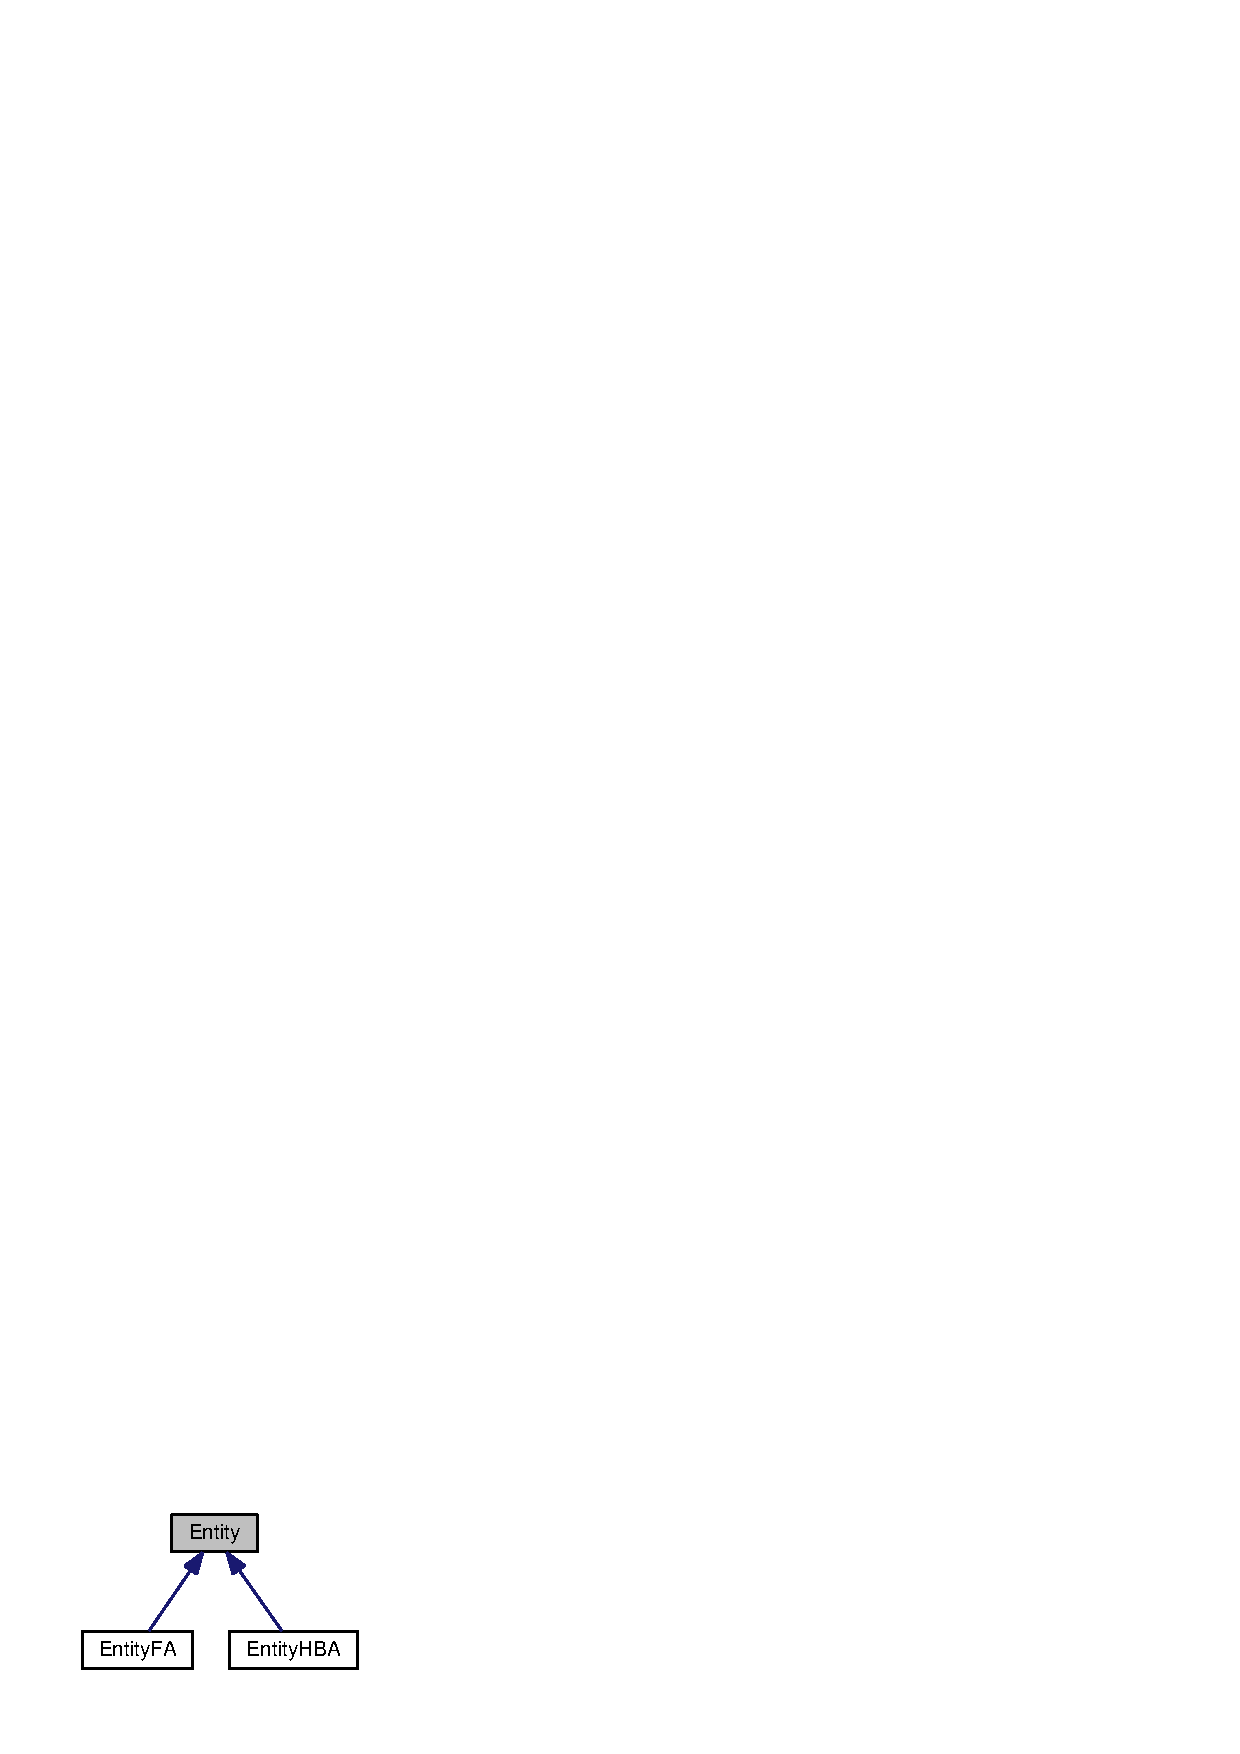
\includegraphics[width=312pt]{classorg_1_1smallfoot_1_1vw4_1_1Entity__inherit__graph}
\end{center}
\end{figure}


Collaboration diagram for Entity\+:\nopagebreak
\begin{figure}[H]
\begin{center}
\leavevmode
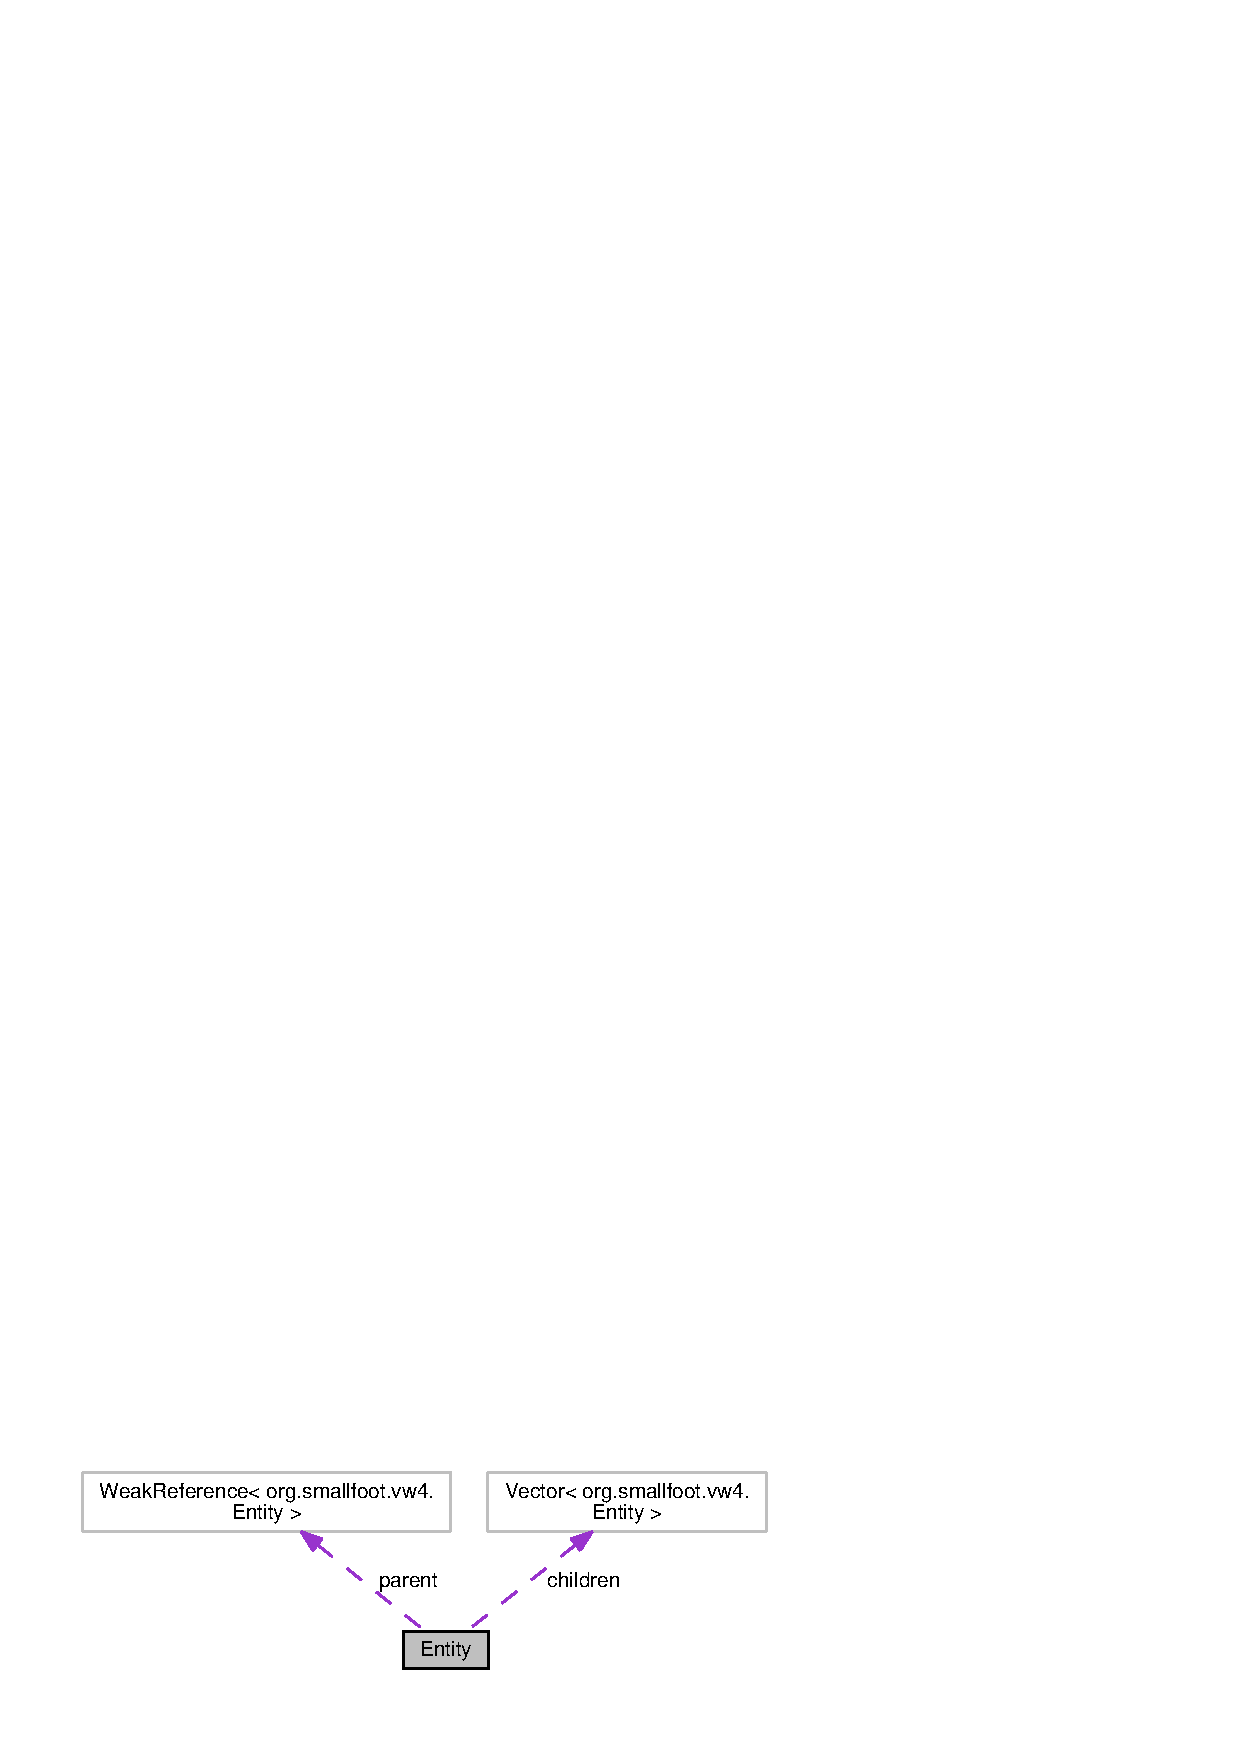
\includegraphics[width=348pt]{classorg_1_1smallfoot_1_1vw4_1_1Entity__coll__graph}
\end{center}
\end{figure}
\subsection*{Data Structures}
\begin{DoxyCompactItemize}
\item 
class {\bf Improper\+Child\+Exception}
\begin{DoxyCompactList}\small\item\em Descendents of \doxyref{Entity}{p.}{classorg_1_1smallfoot_1_1vw4_1_1Entity} should know whether a given entity can be one of their child elements. \end{DoxyCompactList}\item 
class {\bf Leaf\+Entity}
\begin{DoxyCompactList}\small\item\em A \doxyref{Leaf\+Entity}{p.}{classorg_1_1smallfoot_1_1vw4_1_1Entity_1_1LeafEntity} is the common ancestor of Storage F\+As and Server H\+B\+As; this is combined only so that leaves can be treated in common. \end{DoxyCompactList}\end{DoxyCompactItemize}
\subsection*{Public Member Functions}
\begin{DoxyCompactItemize}
\item 
{\bf Entity} (String {\bf name})
\begin{DoxyCompactList}\small\item\em Class Constructor with no initial child. \end{DoxyCompactList}\item 
{\bf Entity} (String {\bf name}, {\bf Entity} e)  throws Improper\+Child\+Exception     
\begin{DoxyCompactList}\small\item\em Class Constructor with an initial child to absorb. \end{DoxyCompactList}\item 
String {\bf description} ()
\begin{DoxyCompactList}\small\item\em the description of the entity showing source \end{DoxyCompactList}\item 
void {\bf maybe\+Adopt} ({\bf Entity} e)  throws Improper\+Child\+Exception     
\begin{DoxyCompactList}\small\item\em Convenience function\+: \doxyref{Entity}{p.}{classorg_1_1smallfoot_1_1vw4_1_1Entity} should either adopt a given child \char`\"{}e\char`\"{} or throw an exception. \end{DoxyCompactList}\item 
String {\bf name} ()
\begin{DoxyCompactList}\small\item\em unique name of the entity\+: getter for internal variable \end{DoxyCompactList}\item 
abstract {\bf Entity} {\bf new\+Parent} (String {\bf name})
\begin{DoxyCompactList}\small\item\em create a new \doxyref{Entity}{p.}{classorg_1_1smallfoot_1_1vw4_1_1Entity} of the correct class to be a parent of this one. \end{DoxyCompactList}\item 
void {\bf set\+Description} (String {\bf description})
\begin{DoxyCompactList}\small\item\em set the description of the entity to show its source\+: setter pattern \end{DoxyCompactList}\item 
void {\bf setname} (String {\bf name})
\begin{DoxyCompactList}\small\item\em set the unique name of the entity\+: setter \end{DoxyCompactList}\end{DoxyCompactItemize}
\subsection*{Static Public Member Functions}
\begin{DoxyCompactItemize}
\item 
static String {\bf compatibility\+Version} ()
\begin{DoxyCompactList}\small\item\em convert the compatibility\+Version into a string \end{DoxyCompactList}\item 
static String {\bf compatibility\+Version} (String new\+Version)
\begin{DoxyCompactList}\small\item\em set a new compatibility string to set a different target version \end{DoxyCompactList}\end{DoxyCompactItemize}
\subsection*{Protected Member Functions}
\begin{DoxyCompactItemize}
\item 
abstract boolean {\bf can\+Be\+Child} ({\bf Entity} e)
\begin{DoxyCompactList}\small\item\em whether a given entity can be this entity's child \end{DoxyCompactList}\item 
Vector$<$ {\bf Entity} $>$ {\bf children} ()
\begin{DoxyCompactList}\small\item\em get a list of child entities (local access to local singleton .children) \end{DoxyCompactList}\item 
abstract \\*
org.\+smallfoot.\+vw4.\+V\+W\+Import.\+Entity {\bf vwentity} (String tag)
\begin{DoxyCompactList}\small\item\em create a streamable J\+S\+O\+N entity from this one \end{DoxyCompactList}\end{DoxyCompactItemize}
\subsection*{Static Protected Member Functions}
\begin{DoxyCompactItemize}
\item 
static int {\bf \+\_\+compatibility\+Version} ()
\begin{DoxyCompactList}\small\item\em calculate the compatibility\+Version as required \end{DoxyCompactList}\end{DoxyCompactItemize}
\subsection*{Protected Attributes}
\begin{DoxyCompactItemize}
\item 
Vector$<$ {\bf Entity} $>$ {\bf children} = null\label{classorg_1_1smallfoot_1_1vw4_1_1Entity_ad315cf5c2790d5a5c8c5169c26647e84}

\begin{DoxyCompactList}\small\item\em local singleton late-\/instantiated as needed by \doxyref{children()}{p.}{classorg_1_1smallfoot_1_1vw4_1_1Entity_a63ef33ad49b88027164e49d1916f409c} \end{DoxyCompactList}\item 
String {\bf description}\label{classorg_1_1smallfoot_1_1vw4_1_1Entity_a76d2b0133d83c43dfd8a19286ac55325}

\begin{DoxyCompactList}\small\item\em the description of the entity showing source \end{DoxyCompactList}\item 
String {\bf name}\label{classorg_1_1smallfoot_1_1vw4_1_1Entity_a9a2326f35466e54c36c070829245c557}

\begin{DoxyCompactList}\small\item\em the unique name of the entity \end{DoxyCompactList}\item 
Weak\+Reference$<$ {\bf Entity} $>$ {\bf parent} = null\label{classorg_1_1smallfoot_1_1vw4_1_1Entity_ab1bf14d6f0f0af84c30272b6eed5792f}

\begin{DoxyCompactList}\small\item\em convenience weak-\/reference to parent\+: I want a reference but not one that will block G\+C \end{DoxyCompactList}\end{DoxyCompactItemize}
\subsection*{Static Protected Attributes}
\begin{DoxyCompactItemize}
\item 
static Integer {\bf compatibility\+Version} = null\label{classorg_1_1smallfoot_1_1vw4_1_1Entity_a30b425bd5034c7ca39be7363c0e86cdc}

\begin{DoxyCompactList}\small\item\em singleton-\/used compatibility\+: if (re)set to null, \doxyref{\+\_\+compatibility\+Version()}{p.}{classorg_1_1smallfoot_1_1vw4_1_1Entity_a2d966176f7b315760e172d3bc03f64a1} recalculates \end{DoxyCompactList}\end{DoxyCompactItemize}


\subsection{Detailed Description}
An \doxyref{Entity}{p.}{classorg_1_1smallfoot_1_1vw4_1_1Entity} is the core mutable object used in the J\+S\+O\+N import for V\+W4. 

I'm not so sure how it'll unfold yet, but I intend to treat all hosts and hbas and storagecontrollers and iomodules as similar objects\+: things that can have children things. In the short term, be very careful\+: there is an \doxyref{Entity}{p.}{classorg_1_1smallfoot_1_1vw4_1_1Entity}, and a V\+W\+Import\+::\+Entity 

Definition at line 46 of file Entity.\+java.



\subsection{Constructor \& Destructor Documentation}
\index{org\+::smallfoot\+::vw4\+::\+Entity@{org\+::smallfoot\+::vw4\+::\+Entity}!Entity@{Entity}}
\index{Entity@{Entity}!org\+::smallfoot\+::vw4\+::\+Entity@{org\+::smallfoot\+::vw4\+::\+Entity}}
\subsubsection[{Entity}]{\setlength{\rightskip}{0pt plus 5cm}{\bf Entity} (
\begin{DoxyParamCaption}
\item[{String}]{name}
\end{DoxyParamCaption}
)\hspace{0.3cm}{\ttfamily [inline]}}\label{classorg_1_1smallfoot_1_1vw4_1_1Entity_afc6a43ee8007bcc023a7ebd2bf5ee1ed}


Class Constructor with no initial child. 


\begin{DoxyParams}{Parameters}
{\em name} & initial name of the new entity \\
\hline
\end{DoxyParams}


Definition at line 196 of file Entity.\+java.



References Entity.\+name().



Here is the call graph for this function\+:\nopagebreak
\begin{figure}[H]
\begin{center}
\leavevmode
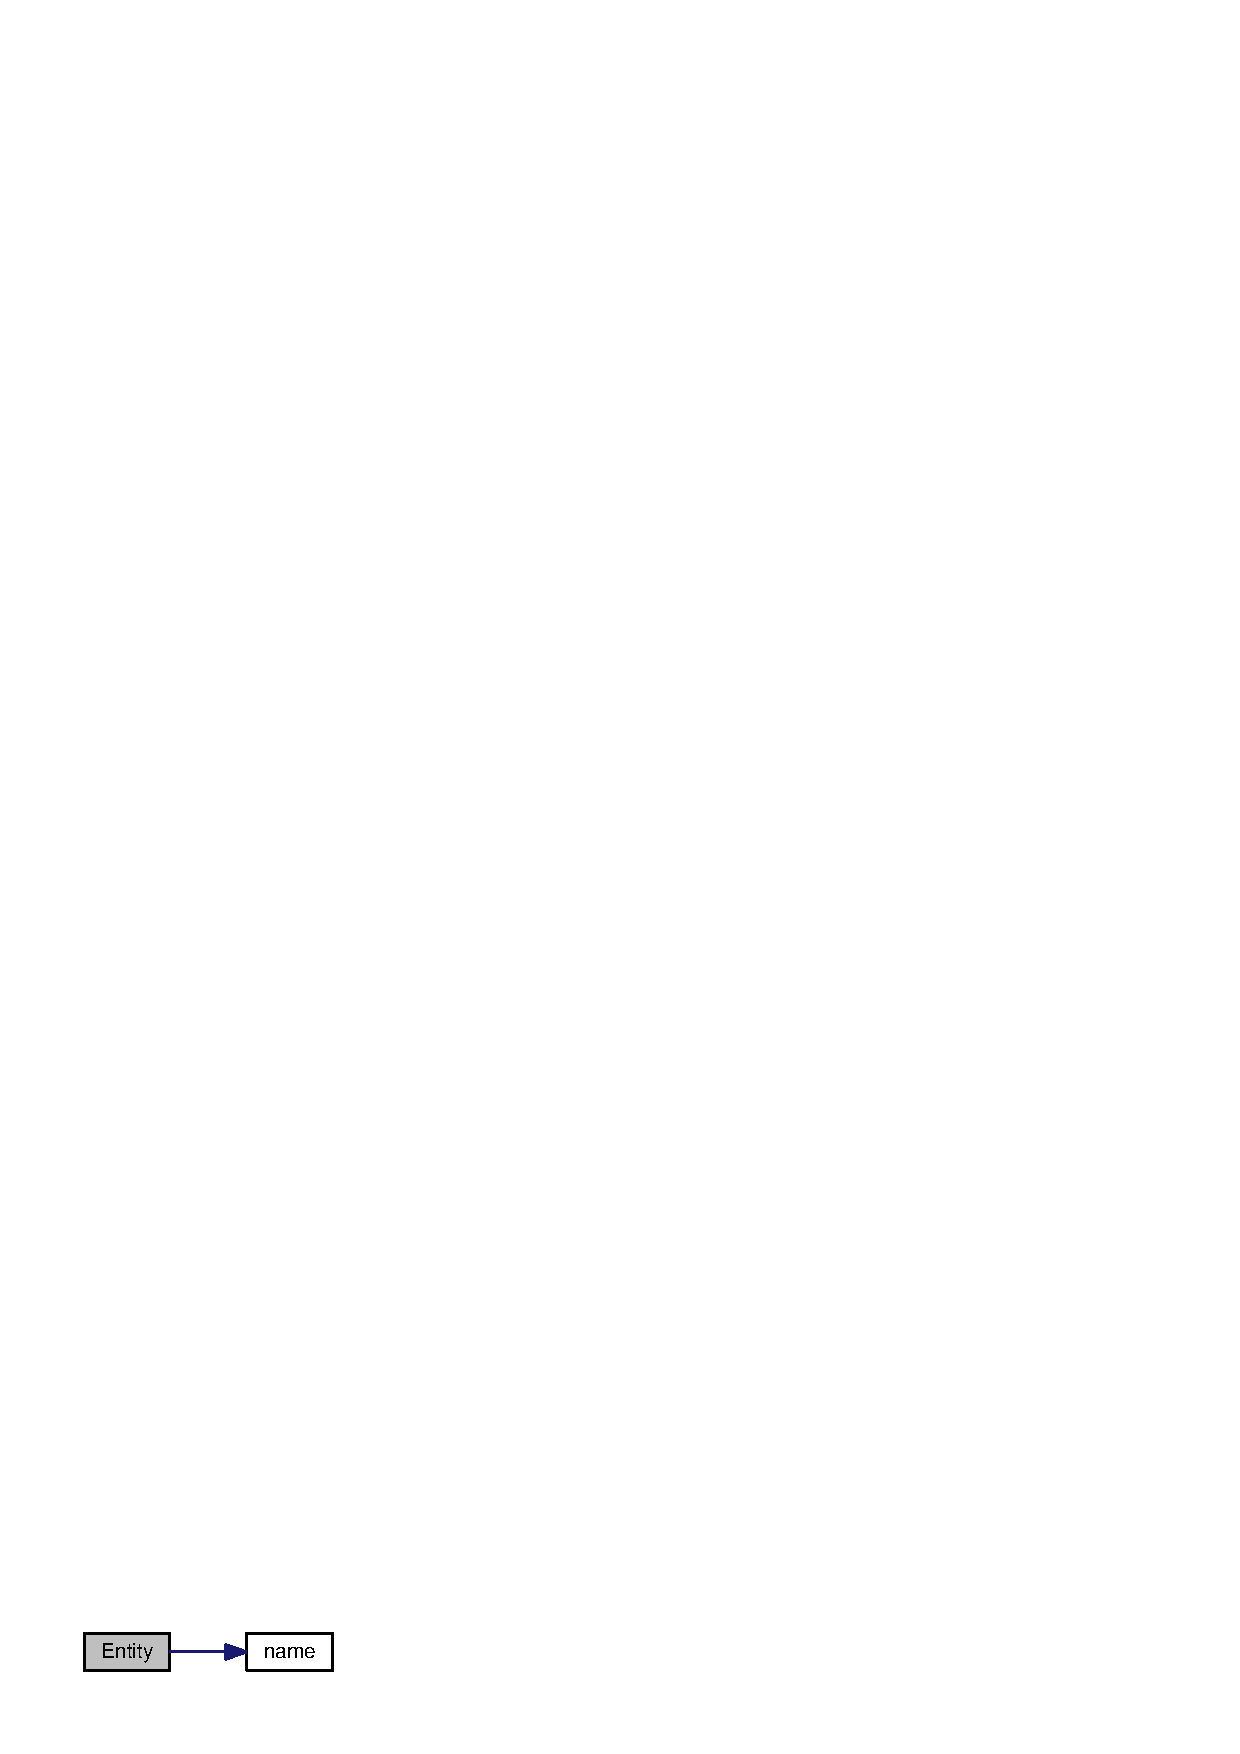
\includegraphics[width=164pt]{classorg_1_1smallfoot_1_1vw4_1_1Entity_afc6a43ee8007bcc023a7ebd2bf5ee1ed_cgraph}
\end{center}
\end{figure}


\index{org\+::smallfoot\+::vw4\+::\+Entity@{org\+::smallfoot\+::vw4\+::\+Entity}!Entity@{Entity}}
\index{Entity@{Entity}!org\+::smallfoot\+::vw4\+::\+Entity@{org\+::smallfoot\+::vw4\+::\+Entity}}
\subsubsection[{Entity}]{\setlength{\rightskip}{0pt plus 5cm}{\bf Entity} (
\begin{DoxyParamCaption}
\item[{String}]{name, }
\item[{{\bf Entity}}]{e}
\end{DoxyParamCaption}
) throws {\bf Improper\+Child\+Exception}\hspace{0.3cm}{\ttfamily [inline]}}\label{classorg_1_1smallfoot_1_1vw4_1_1Entity_a1afb3a328033f8f6bf136d8380e712b9}


Class Constructor with an initial child to absorb. 


\begin{DoxyParams}{Parameters}
{\em name} & initial name of the new entity \\
\hline
{\em e} & \doxyref{Entity}{p.}{classorg_1_1smallfoot_1_1vw4_1_1Entity} to consider for adoption as child \\
\hline
\end{DoxyParams}


Definition at line 207 of file Entity.\+java.



References Entity.\+maybe\+Adopt(), and Entity.\+name().



Here is the call graph for this function\+:\nopagebreak
\begin{figure}[H]
\begin{center}
\leavevmode
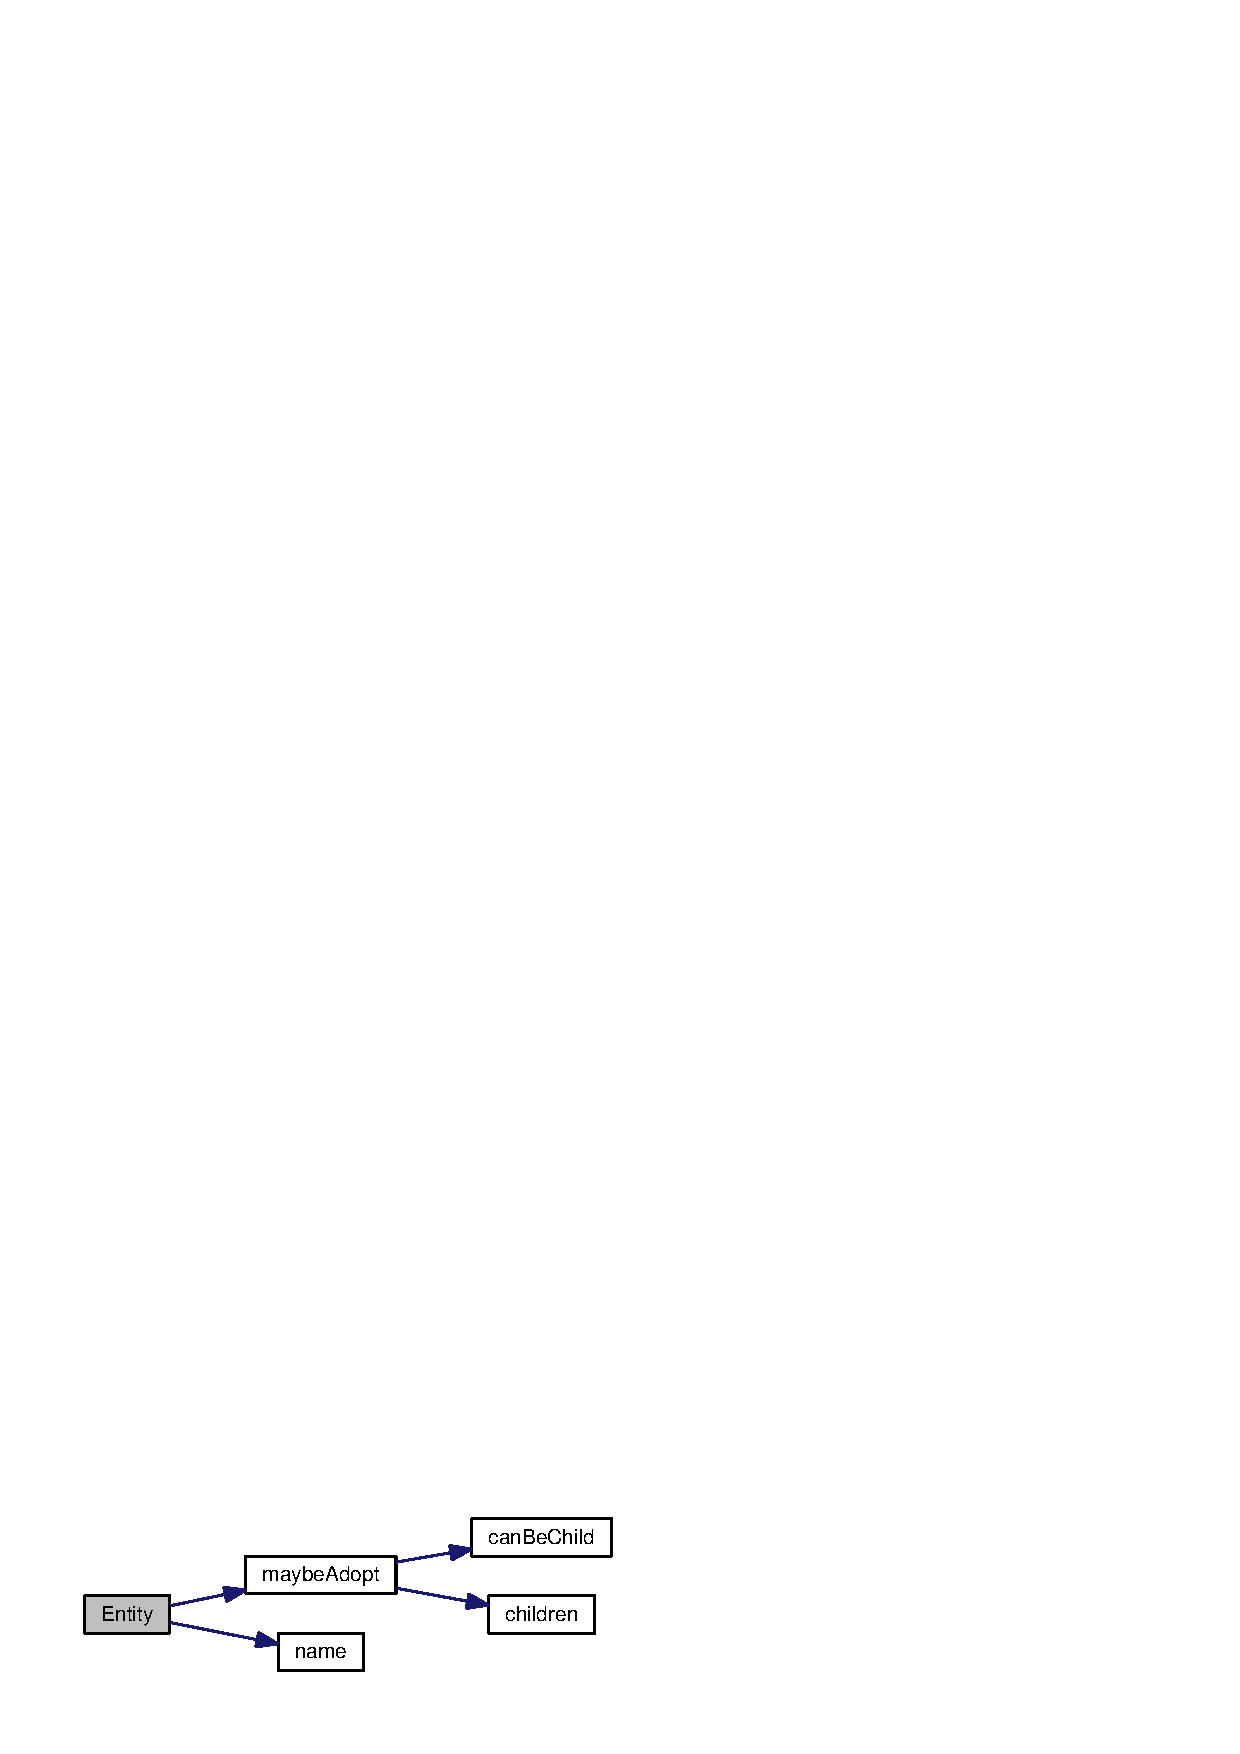
\includegraphics[width=298pt]{classorg_1_1smallfoot_1_1vw4_1_1Entity_a1afb3a328033f8f6bf136d8380e712b9_cgraph}
\end{center}
\end{figure}




\subsection{Member Function Documentation}
\index{org\+::smallfoot\+::vw4\+::\+Entity@{org\+::smallfoot\+::vw4\+::\+Entity}!\+\_\+compatibility\+Version@{\+\_\+compatibility\+Version}}
\index{\+\_\+compatibility\+Version@{\+\_\+compatibility\+Version}!org\+::smallfoot\+::vw4\+::\+Entity@{org\+::smallfoot\+::vw4\+::\+Entity}}
\subsubsection[{\+\_\+compatibility\+Version}]{\setlength{\rightskip}{0pt plus 5cm}static int \+\_\+compatibility\+Version (
\begin{DoxyParamCaption}
{}
\end{DoxyParamCaption}
)\hspace{0.3cm}{\ttfamily [inline]}, {\ttfamily [static]}, {\ttfamily [protected]}}\label{classorg_1_1smallfoot_1_1vw4_1_1Entity_a2d966176f7b315760e172d3bc03f64a1}


calculate the compatibility\+Version as required 

\begin{DoxyReturn}{Returns}
integer value of compatibility\+Version
\end{DoxyReturn}
\begin{DoxyRefDesc}{J\+V\+M Options}
\item[{\bf J\+V\+M Options}]{\bfseries compat.\+target} (values\+: X.\+Y.\+Z as a version. For example\+: 4.\+0.\+1, 4.\+1, 4, 4.\+2) can be used to tell the J\+S\+O\+N output to use specific features available on later versions of the Virtual\+Wisdom4 product. Initially controls whether fcport entities are created but may expand. \end{DoxyRefDesc}


Definition at line 58 of file Entity.\+java.



References Entity.\+compatibility\+Version().



Referenced by Entity.\+compatibility\+Version(), Entity\+H\+B\+A.\+vwentity(), and Entity\+F\+A.\+vwentity().



Here is the call graph for this function\+:\nopagebreak
\begin{figure}[H]
\begin{center}
\leavevmode
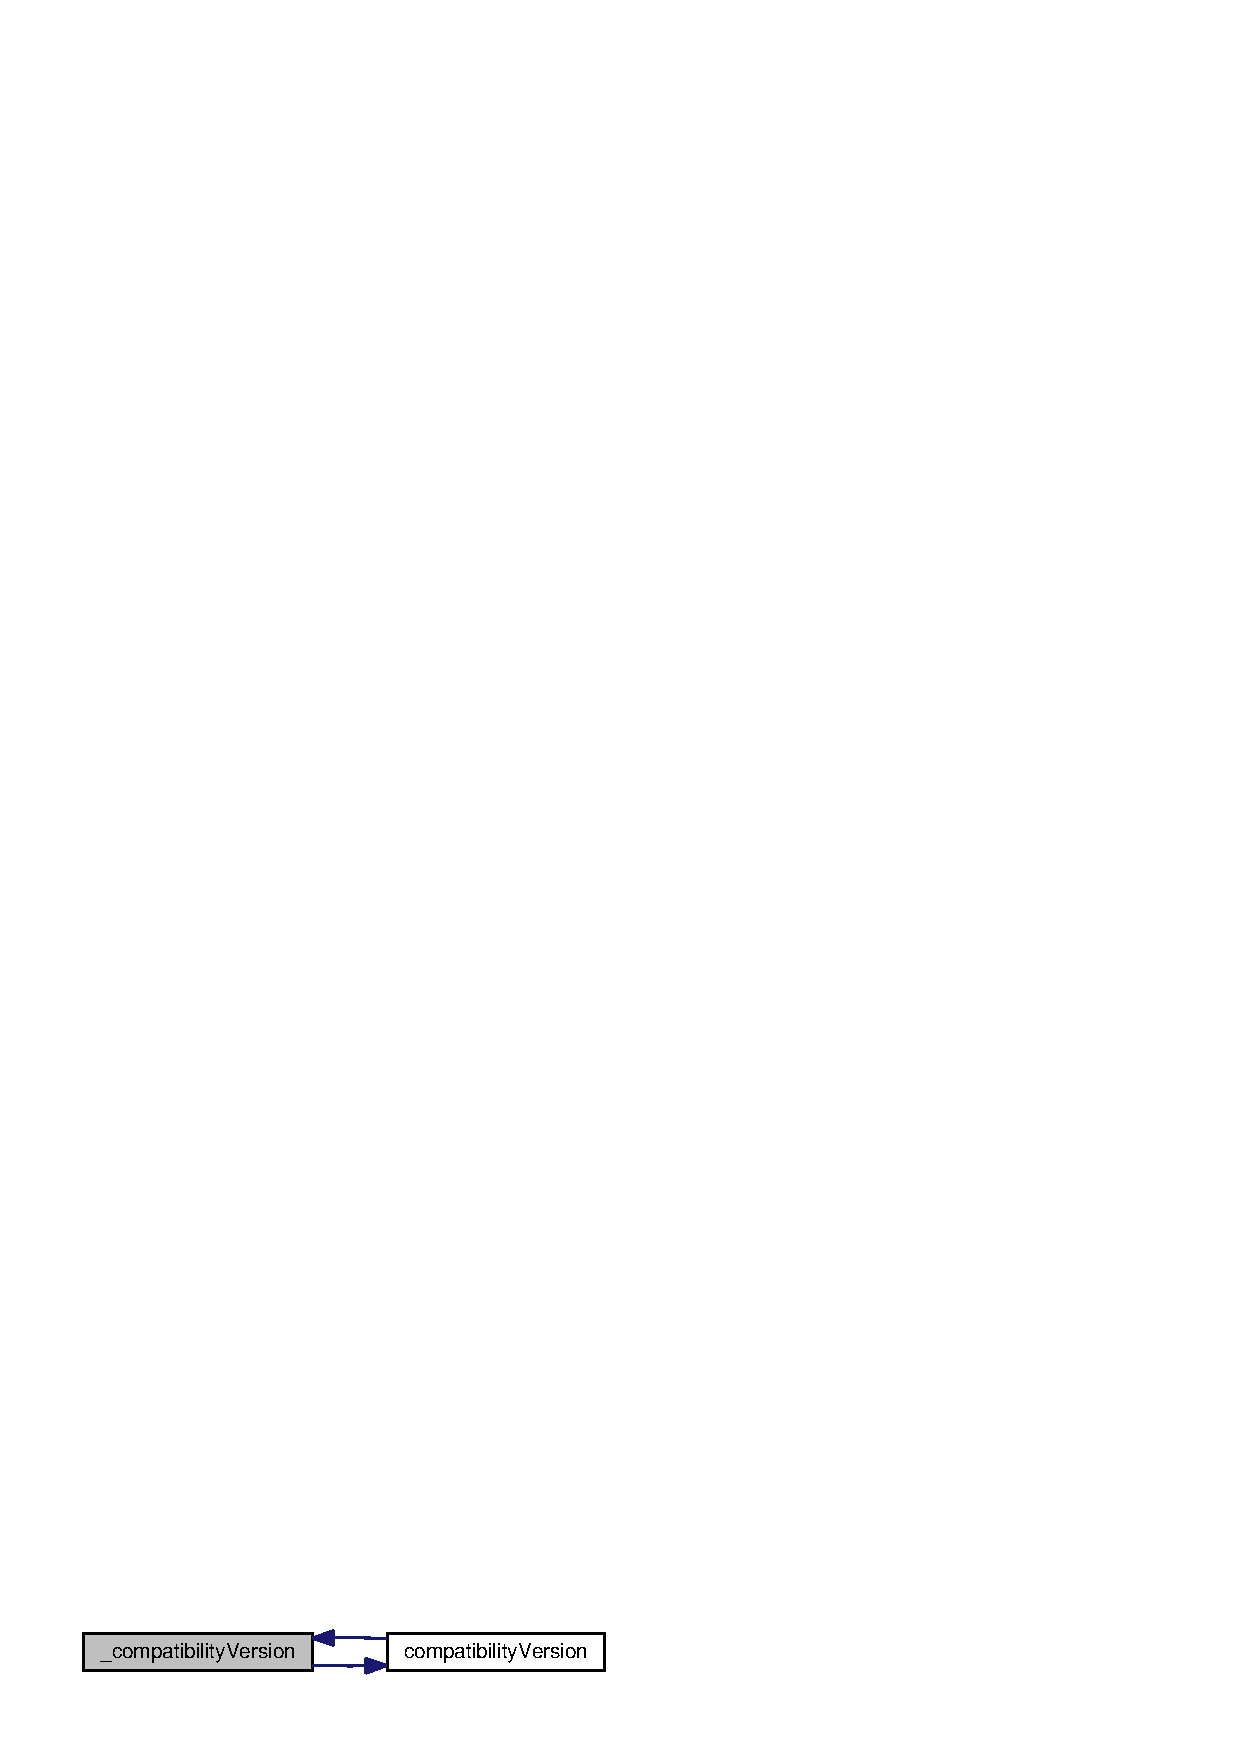
\includegraphics[width=294pt]{classorg_1_1smallfoot_1_1vw4_1_1Entity_a2d966176f7b315760e172d3bc03f64a1_cgraph}
\end{center}
\end{figure}


\index{org\+::smallfoot\+::vw4\+::\+Entity@{org\+::smallfoot\+::vw4\+::\+Entity}!can\+Be\+Child@{can\+Be\+Child}}
\index{can\+Be\+Child@{can\+Be\+Child}!org\+::smallfoot\+::vw4\+::\+Entity@{org\+::smallfoot\+::vw4\+::\+Entity}}
\subsubsection[{can\+Be\+Child}]{\setlength{\rightskip}{0pt plus 5cm}abstract boolean can\+Be\+Child (
\begin{DoxyParamCaption}
\item[{{\bf Entity}}]{e}
\end{DoxyParamCaption}
)\hspace{0.3cm}{\ttfamily [abstract]}, {\ttfamily [protected]}}\label{classorg_1_1smallfoot_1_1vw4_1_1Entity_a0a8c67a491e7100ba94f3035bbe62822}


whether a given entity can be this entity's child 


\begin{DoxyParams}{Parameters}
{\em e} & entity to check for possible descendent-\/hood \\
\hline
\end{DoxyParams}
\begin{DoxyReturn}{Returns}
true if this entity accepts children of \char`\"{}e\char`\"{}'s descendent type 
\end{DoxyReturn}


Referenced by Entity.\+maybe\+Adopt().

\index{org\+::smallfoot\+::vw4\+::\+Entity@{org\+::smallfoot\+::vw4\+::\+Entity}!children@{children}}
\index{children@{children}!org\+::smallfoot\+::vw4\+::\+Entity@{org\+::smallfoot\+::vw4\+::\+Entity}}
\subsubsection[{children}]{\setlength{\rightskip}{0pt plus 5cm}Vector$<${\bf Entity}$>$ children (
\begin{DoxyParamCaption}
{}
\end{DoxyParamCaption}
)\hspace{0.3cm}{\ttfamily [inline]}, {\ttfamily [protected]}}\label{classorg_1_1smallfoot_1_1vw4_1_1Entity_a63ef33ad49b88027164e49d1916f409c}


get a list of child entities (local access to local singleton .children) 

\begin{DoxyReturn}{Returns}
list of zero or more child entities but never null 
\end{DoxyReturn}


Definition at line 140 of file Entity.\+java.



Referenced by Entity.\+maybe\+Adopt(), Entity\+Host.\+vwentity(), and Entity\+Array.\+vwentity().

\index{org\+::smallfoot\+::vw4\+::\+Entity@{org\+::smallfoot\+::vw4\+::\+Entity}!compatibility\+Version@{compatibility\+Version}}
\index{compatibility\+Version@{compatibility\+Version}!org\+::smallfoot\+::vw4\+::\+Entity@{org\+::smallfoot\+::vw4\+::\+Entity}}
\subsubsection[{compatibility\+Version}]{\setlength{\rightskip}{0pt plus 5cm}static String compatibility\+Version (
\begin{DoxyParamCaption}
{}
\end{DoxyParamCaption}
)\hspace{0.3cm}{\ttfamily [inline]}, {\ttfamily [static]}}\label{classorg_1_1smallfoot_1_1vw4_1_1Entity_aafad8b8b69f1c940a90bb5e2ef672ebf}


convert the compatibility\+Version into a string 

\begin{DoxyReturn}{Returns}
string value of compatibility\+Version 
\end{DoxyReturn}


Definition at line 95 of file Entity.\+java.



References Entity.\+\_\+compatibility\+Version().



Referenced by Entity.\+\_\+compatibility\+Version(), and Entity.\+compatibility\+Version().



Here is the call graph for this function\+:\nopagebreak
\begin{figure}[H]
\begin{center}
\leavevmode
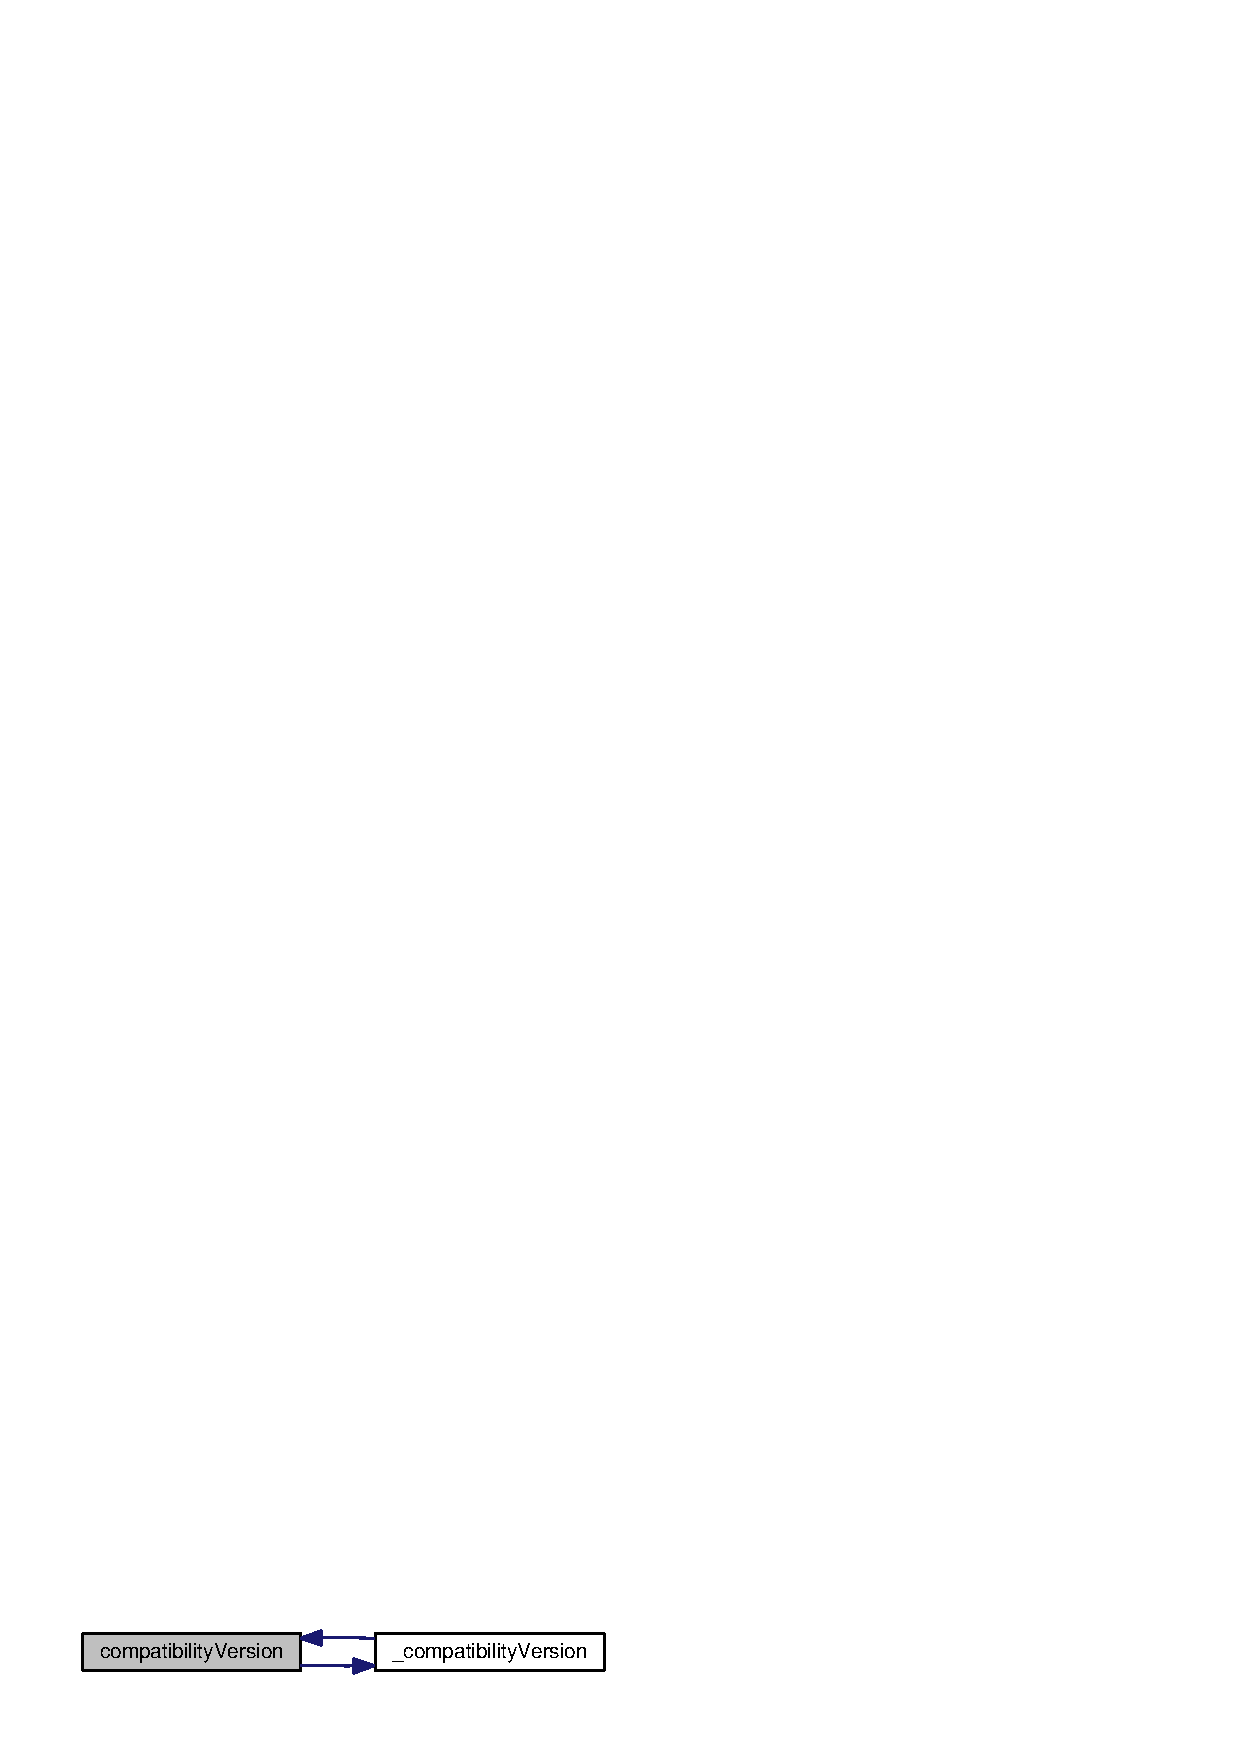
\includegraphics[width=294pt]{classorg_1_1smallfoot_1_1vw4_1_1Entity_aafad8b8b69f1c940a90bb5e2ef672ebf_cgraph}
\end{center}
\end{figure}


\index{org\+::smallfoot\+::vw4\+::\+Entity@{org\+::smallfoot\+::vw4\+::\+Entity}!compatibility\+Version@{compatibility\+Version}}
\index{compatibility\+Version@{compatibility\+Version}!org\+::smallfoot\+::vw4\+::\+Entity@{org\+::smallfoot\+::vw4\+::\+Entity}}
\subsubsection[{compatibility\+Version}]{\setlength{\rightskip}{0pt plus 5cm}static String compatibility\+Version (
\begin{DoxyParamCaption}
\item[{String}]{new\+Version}
\end{DoxyParamCaption}
)\hspace{0.3cm}{\ttfamily [inline]}, {\ttfamily [static]}}\label{classorg_1_1smallfoot_1_1vw4_1_1Entity_aa3f7ad2834fa542cf7d5cc554c49677d}


set a new compatibility string to set a different target version 

This, with \doxyref{compatibility\+Version()}{p.}{classorg_1_1smallfoot_1_1vw4_1_1Entity_aafad8b8b69f1c940a90bb5e2ef672ebf} and \doxyref{\+\_\+compatibility\+Version()}{p.}{classorg_1_1smallfoot_1_1vw4_1_1Entity_a2d966176f7b315760e172d3bc03f64a1}, is a lot of scaffolding around compatibility outputs; I'm both trying to give some versatility here, plus experimenting myself with properties-\/vs-\/commandlines-\/vs-\/both. At the end of the day, both methods work to set a version for output, initially a determiner whether fcport entities are produced. There's future possibility for growth, including config/properties files, afforded by this massive 4-\/part scaffolding with delusions of grandeur.


\begin{DoxyParams}{Parameters}
{\em new\+Version} & the new value to use as a version\\
\hline
\end{DoxyParams}
\begin{DoxyReturn}{Returns}
previous config version 
\end{DoxyReturn}


Definition at line 114 of file Entity.\+java.



References Entity.\+compatibility\+Version().



Here is the call graph for this function\+:\nopagebreak
\begin{figure}[H]
\begin{center}
\leavevmode
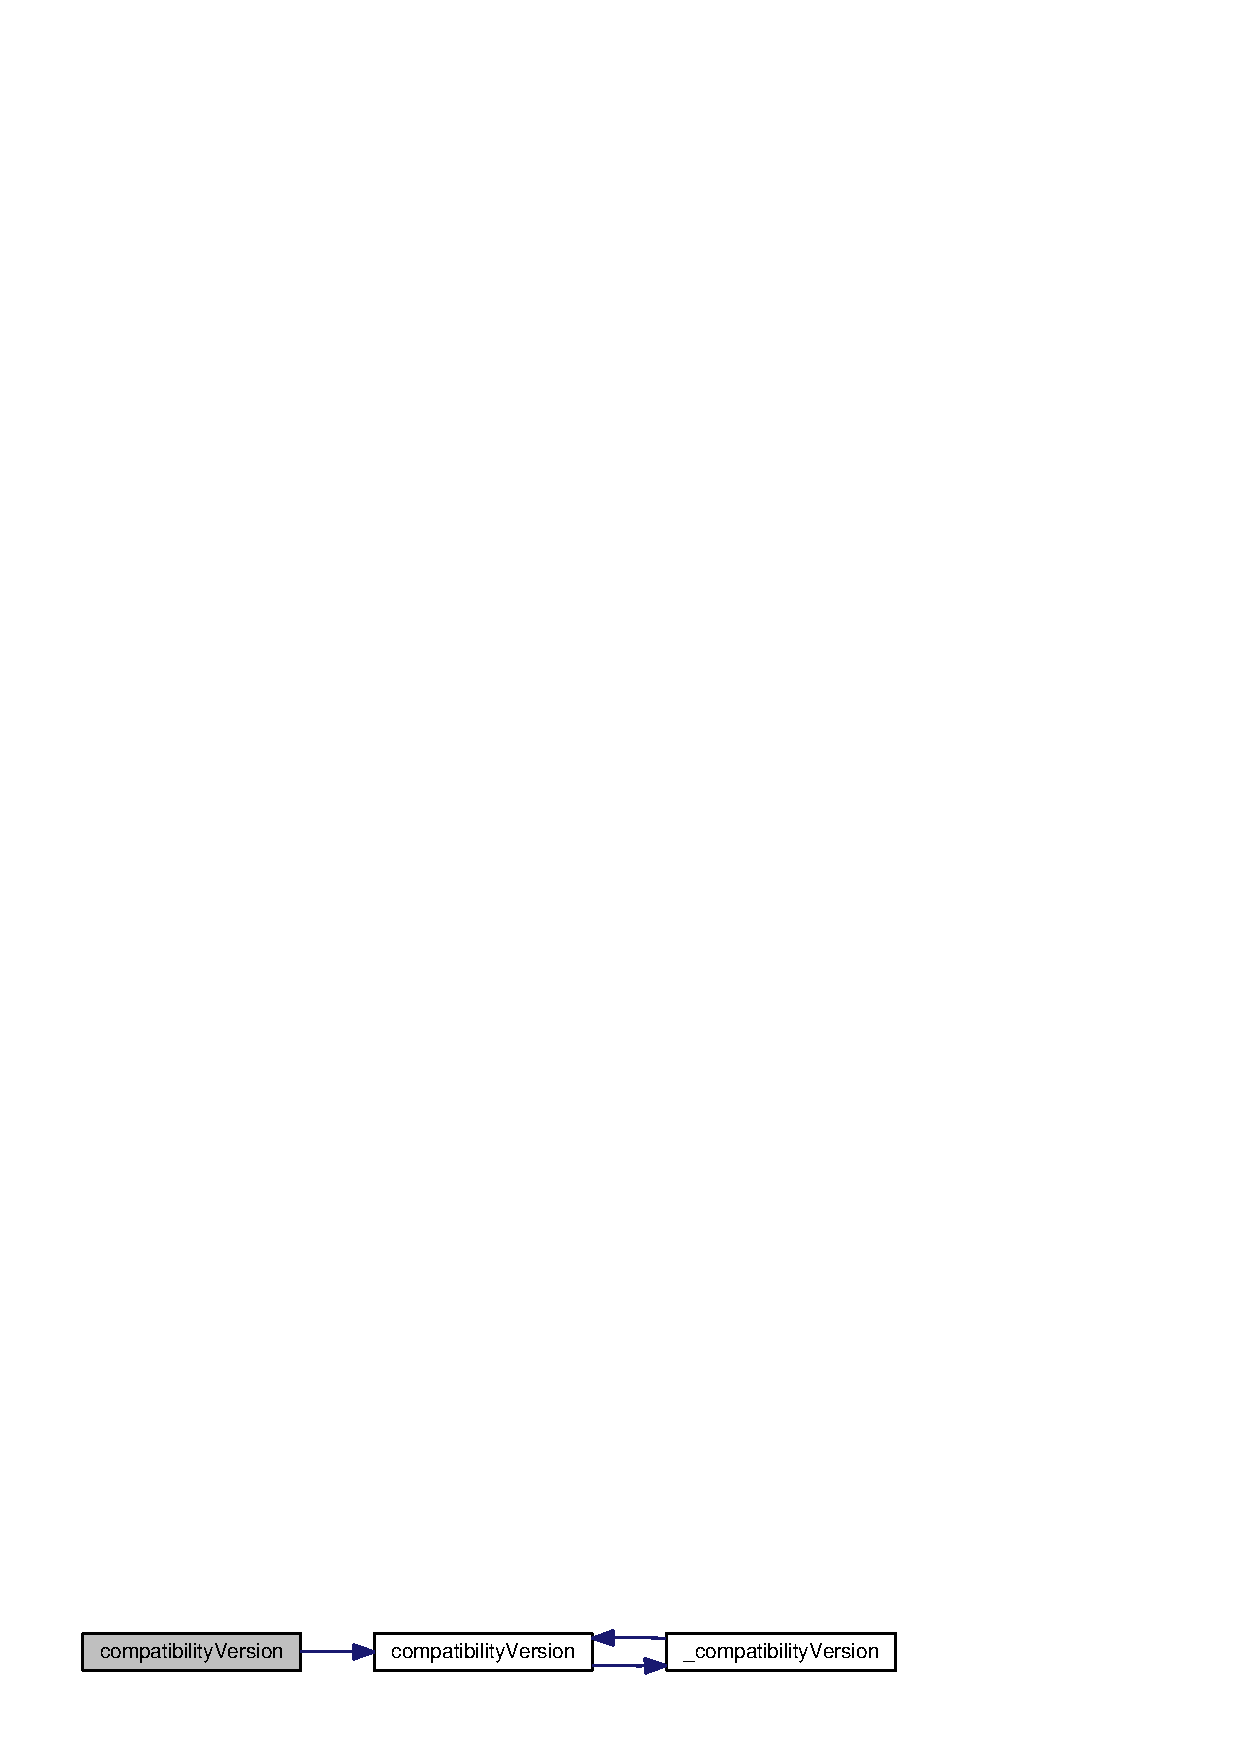
\includegraphics[width=350pt]{classorg_1_1smallfoot_1_1vw4_1_1Entity_aa3f7ad2834fa542cf7d5cc554c49677d_cgraph}
\end{center}
\end{figure}


\index{org\+::smallfoot\+::vw4\+::\+Entity@{org\+::smallfoot\+::vw4\+::\+Entity}!description@{description}}
\index{description@{description}!org\+::smallfoot\+::vw4\+::\+Entity@{org\+::smallfoot\+::vw4\+::\+Entity}}
\subsubsection[{description}]{\setlength{\rightskip}{0pt plus 5cm}String description (
\begin{DoxyParamCaption}
{}
\end{DoxyParamCaption}
)\hspace{0.3cm}{\ttfamily [inline]}}\label{classorg_1_1smallfoot_1_1vw4_1_1Entity_a464a9940ad720e717c25422b41b7845b}


the description of the entity showing source 

\begin{DoxyReturn}{Returns}
description of the entity 
\end{DoxyReturn}


Definition at line 160 of file Entity.\+java.



Referenced by Entity.\+set\+Description(), Entity\+H\+B\+A.\+vwentity(), Entity\+F\+A.\+vwentity(), Entity\+Array.\+vwentity(), and Entity\+Host.\+vwentity().

\index{org\+::smallfoot\+::vw4\+::\+Entity@{org\+::smallfoot\+::vw4\+::\+Entity}!maybe\+Adopt@{maybe\+Adopt}}
\index{maybe\+Adopt@{maybe\+Adopt}!org\+::smallfoot\+::vw4\+::\+Entity@{org\+::smallfoot\+::vw4\+::\+Entity}}
\subsubsection[{maybe\+Adopt}]{\setlength{\rightskip}{0pt plus 5cm}void maybe\+Adopt (
\begin{DoxyParamCaption}
\item[{{\bf Entity}}]{e}
\end{DoxyParamCaption}
) throws {\bf Improper\+Child\+Exception}\hspace{0.3cm}{\ttfamily [inline]}}\label{classorg_1_1smallfoot_1_1vw4_1_1Entity_abeab35e912fa1da9e137231518b27e19}


Convenience function\+: \doxyref{Entity}{p.}{classorg_1_1smallfoot_1_1vw4_1_1Entity} should either adopt a given child \char`\"{}e\char`\"{} or throw an exception. 

This allows very simple coding of streamlining the adoption in a cleaner iteration loop.


\begin{DoxyParams}{Parameters}
{\em e} & \doxyref{Entity}{p.}{classorg_1_1smallfoot_1_1vw4_1_1Entity} to consider for adoption as child \\
\hline
\end{DoxyParams}


Definition at line 218 of file Entity.\+java.



References Entity.\+can\+Be\+Child(), Entity.\+children(), and Entity.\+parent.



Referenced by Entity.\+Entity().



Here is the call graph for this function\+:\nopagebreak
\begin{figure}[H]
\begin{center}
\leavevmode
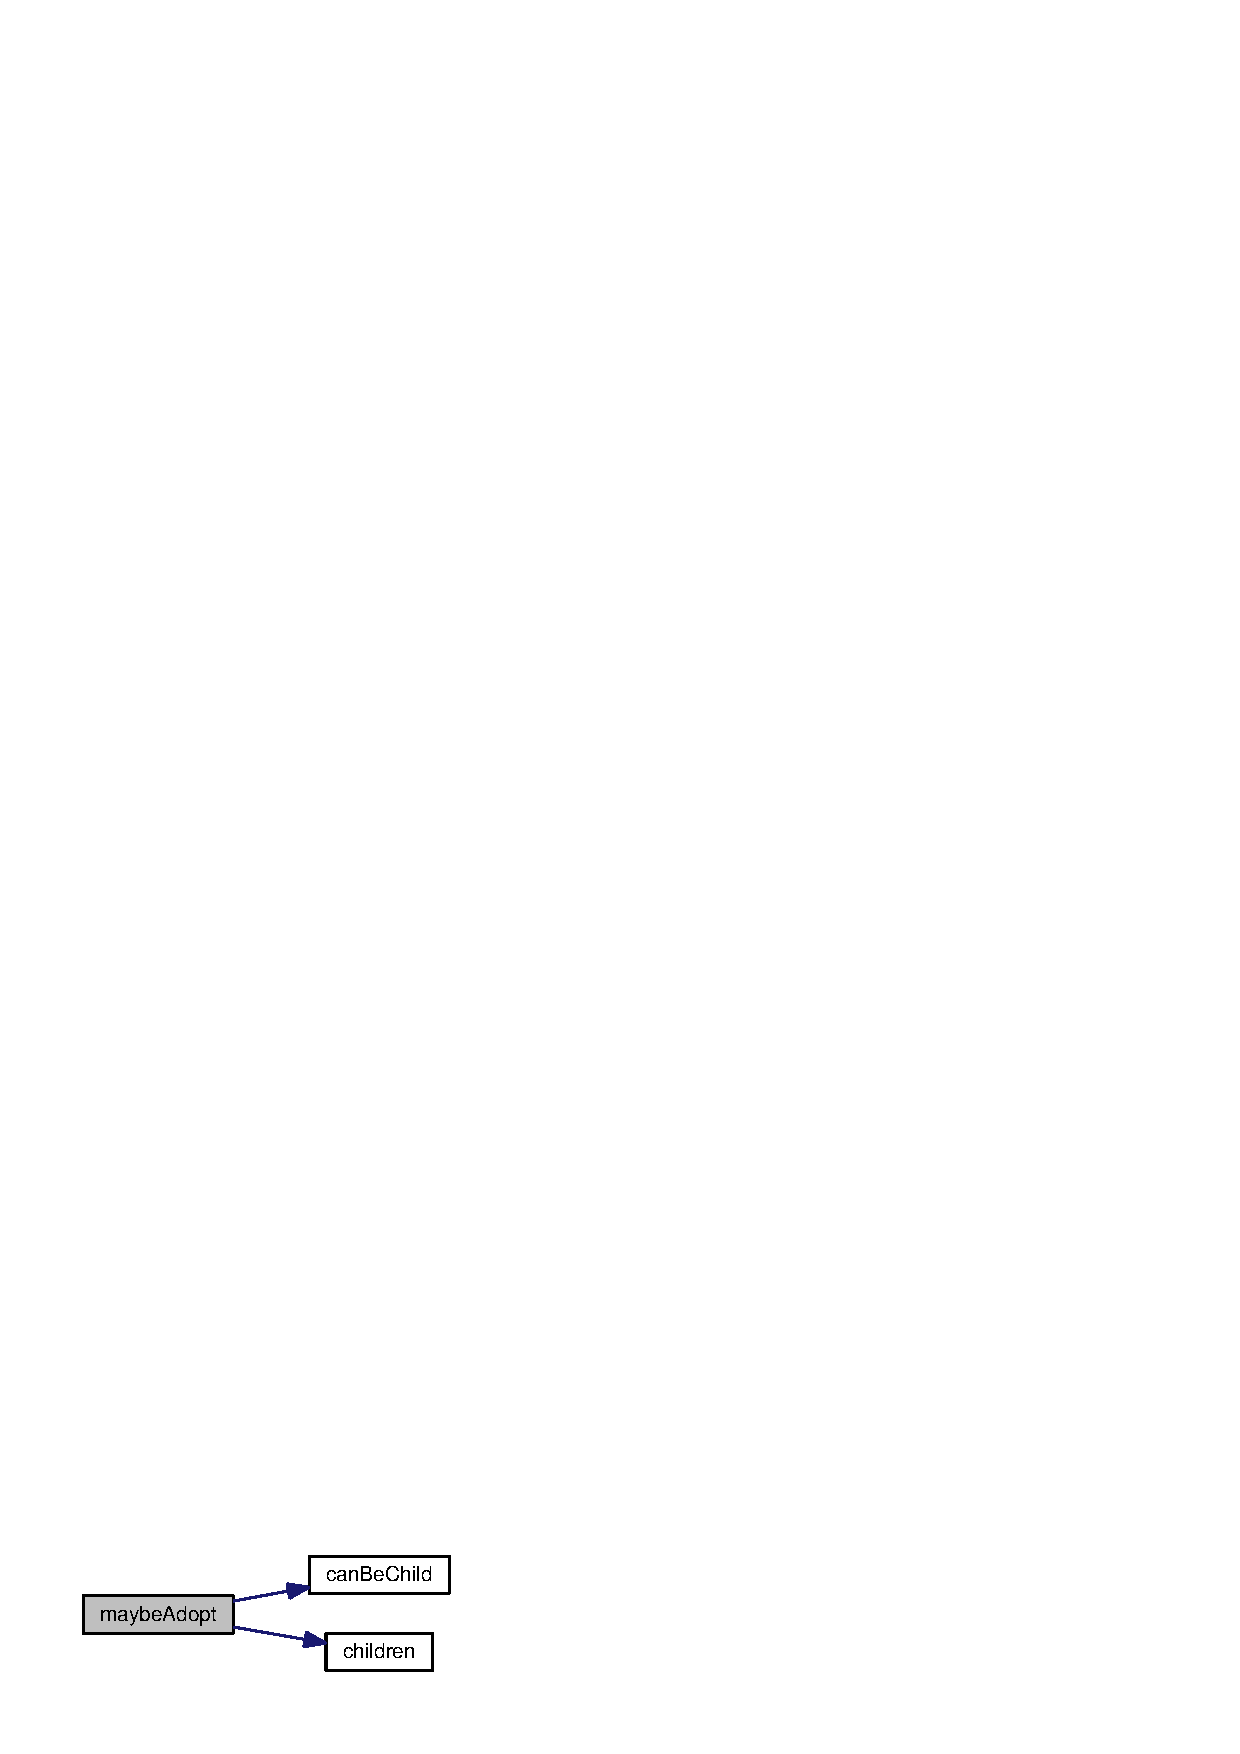
\includegraphics[width=220pt]{classorg_1_1smallfoot_1_1vw4_1_1Entity_abeab35e912fa1da9e137231518b27e19_cgraph}
\end{center}
\end{figure}


\index{org\+::smallfoot\+::vw4\+::\+Entity@{org\+::smallfoot\+::vw4\+::\+Entity}!name@{name}}
\index{name@{name}!org\+::smallfoot\+::vw4\+::\+Entity@{org\+::smallfoot\+::vw4\+::\+Entity}}
\subsubsection[{name}]{\setlength{\rightskip}{0pt plus 5cm}String name (
\begin{DoxyParamCaption}
{}
\end{DoxyParamCaption}
)\hspace{0.3cm}{\ttfamily [inline]}}\label{classorg_1_1smallfoot_1_1vw4_1_1Entity_afa2149aced9d90555f788dfc81c23d15}


unique name of the entity\+: getter for internal variable 

\begin{DoxyReturn}{Returns}
the name 
\end{DoxyReturn}


Definition at line 148 of file Entity.\+java.



Referenced by Entity.\+Entity(), Entity\+Array.\+Entity\+Array(), Entity\+Host.\+Entity\+Host(), Entity.\+Leaf\+Entity.\+parent\+Name(), Entity.\+setname(), Entity\+F\+A.\+vwentity(), Entity\+H\+B\+A.\+vwentity(), Entity\+Host.\+vwentity(), and Entity\+Array.\+vwentity().

\index{org\+::smallfoot\+::vw4\+::\+Entity@{org\+::smallfoot\+::vw4\+::\+Entity}!new\+Parent@{new\+Parent}}
\index{new\+Parent@{new\+Parent}!org\+::smallfoot\+::vw4\+::\+Entity@{org\+::smallfoot\+::vw4\+::\+Entity}}
\subsubsection[{new\+Parent}]{\setlength{\rightskip}{0pt plus 5cm}abstract {\bf Entity} new\+Parent (
\begin{DoxyParamCaption}
\item[{String}]{name}
\end{DoxyParamCaption}
)\hspace{0.3cm}{\ttfamily [abstract]}}\label{classorg_1_1smallfoot_1_1vw4_1_1Entity_a09bc887ffb8f12a369fd5f5da7cfef31}


create a new \doxyref{Entity}{p.}{classorg_1_1smallfoot_1_1vw4_1_1Entity} of the correct class to be a parent of this one. 

This function is used to polymorphically create the parentage of an entity such as the host holding an H\+B\+A

\begin{DoxyReturn}{Returns}
new parent for this entity 
\end{DoxyReturn}

\begin{DoxyParams}{Parameters}
{\em name} & initial name of the new entity \\
\hline
\end{DoxyParams}
\index{org\+::smallfoot\+::vw4\+::\+Entity@{org\+::smallfoot\+::vw4\+::\+Entity}!set\+Description@{set\+Description}}
\index{set\+Description@{set\+Description}!org\+::smallfoot\+::vw4\+::\+Entity@{org\+::smallfoot\+::vw4\+::\+Entity}}
\subsubsection[{set\+Description}]{\setlength{\rightskip}{0pt plus 5cm}void set\+Description (
\begin{DoxyParamCaption}
\item[{String}]{description}
\end{DoxyParamCaption}
)\hspace{0.3cm}{\ttfamily [inline]}}\label{classorg_1_1smallfoot_1_1vw4_1_1Entity_a1d15d718177c4f5411ce6ab339889fd4}


set the description of the entity to show its source\+: setter pattern 


\begin{DoxyParams}{Parameters}
{\em description} & the description to set \\
\hline
\end{DoxyParams}


Definition at line 165 of file Entity.\+java.



References Entity.\+description().



Referenced by Virtual\+Wisdom4\+Client\+Tool.\+load\+And\+Absorb\+File().



Here is the call graph for this function\+:\nopagebreak
\begin{figure}[H]
\begin{center}
\leavevmode
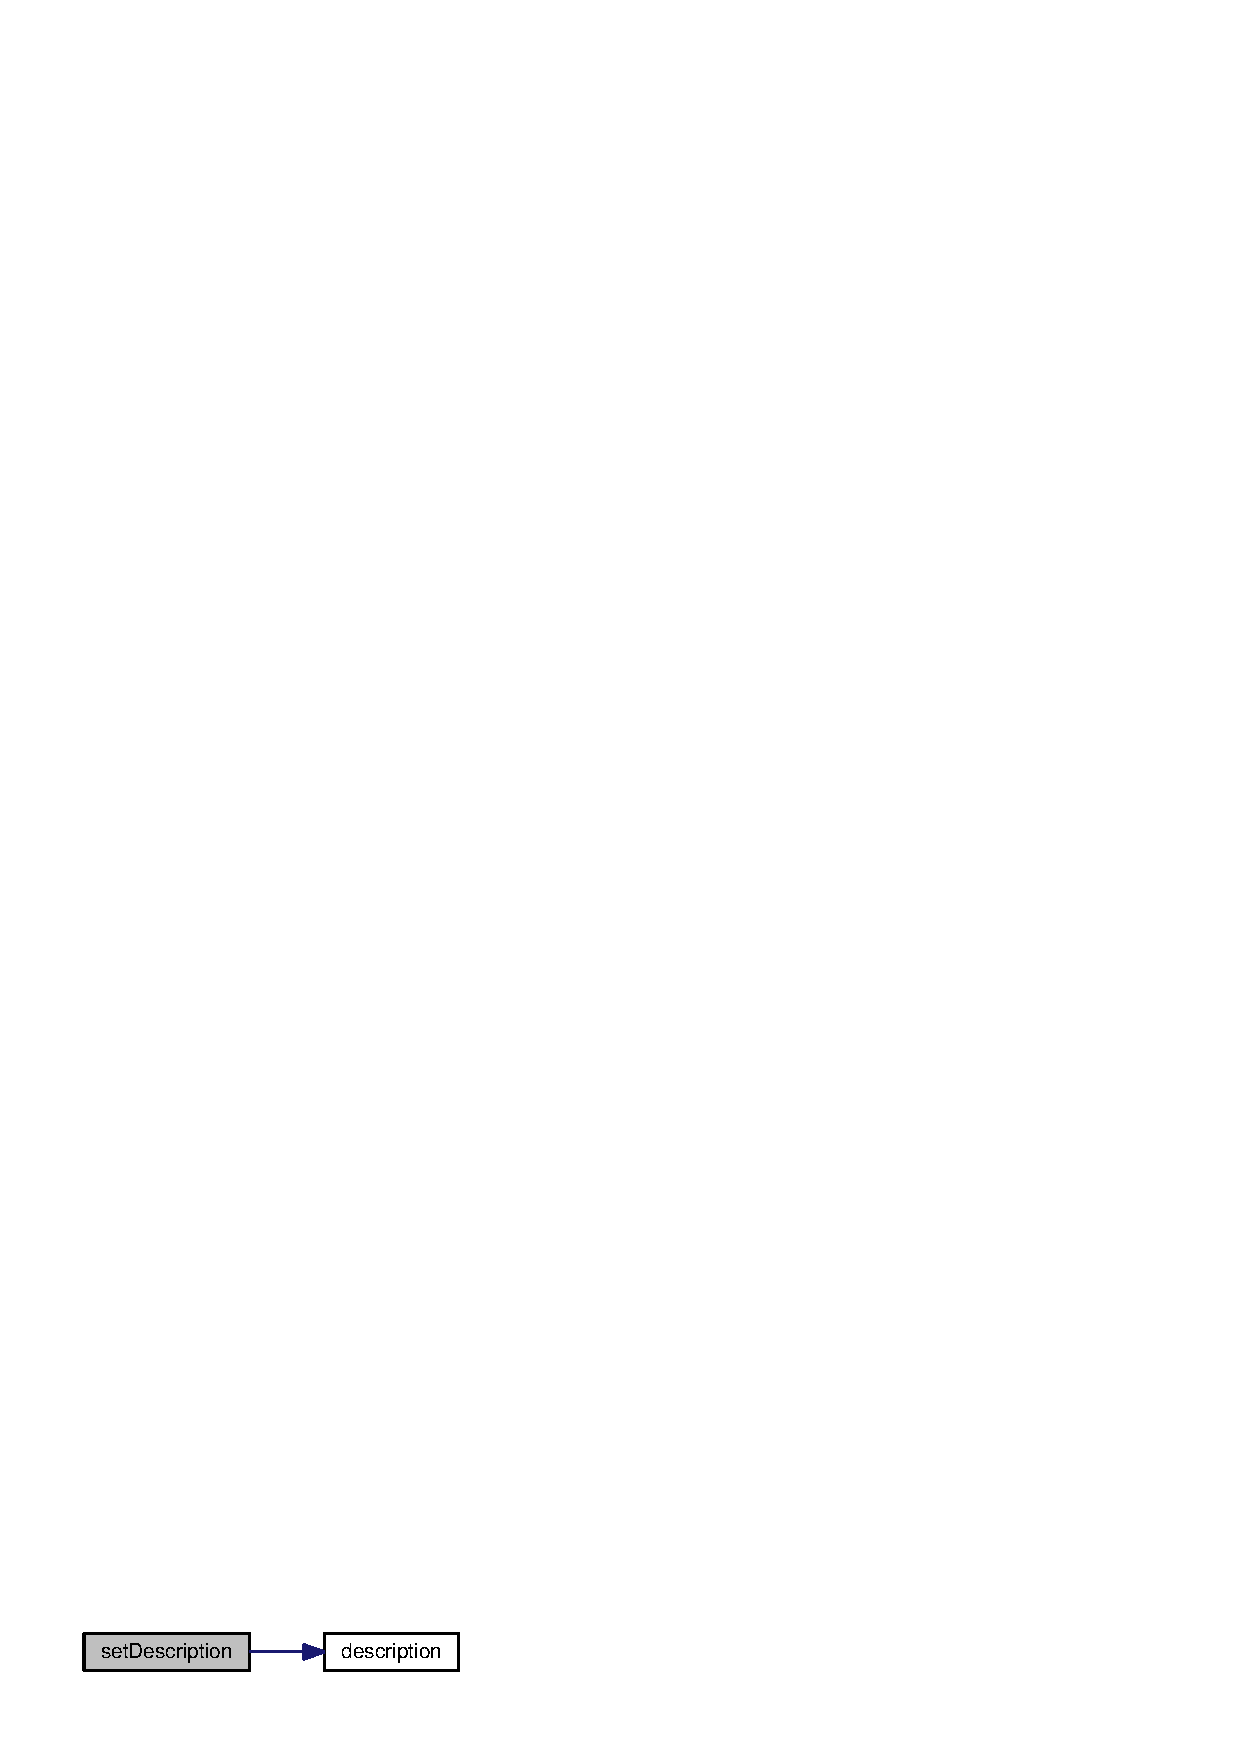
\includegraphics[width=224pt]{classorg_1_1smallfoot_1_1vw4_1_1Entity_a1d15d718177c4f5411ce6ab339889fd4_cgraph}
\end{center}
\end{figure}


\index{org\+::smallfoot\+::vw4\+::\+Entity@{org\+::smallfoot\+::vw4\+::\+Entity}!setname@{setname}}
\index{setname@{setname}!org\+::smallfoot\+::vw4\+::\+Entity@{org\+::smallfoot\+::vw4\+::\+Entity}}
\subsubsection[{setname}]{\setlength{\rightskip}{0pt plus 5cm}void setname (
\begin{DoxyParamCaption}
\item[{String}]{name}
\end{DoxyParamCaption}
)\hspace{0.3cm}{\ttfamily [inline]}}\label{classorg_1_1smallfoot_1_1vw4_1_1Entity_a670f83b1f0f39a20e0fe60597032a367}


set the unique name of the entity\+: setter 


\begin{DoxyParams}{Parameters}
{\em name} & the name to set \\
\hline
\end{DoxyParams}


Definition at line 153 of file Entity.\+java.



References Entity.\+name().



Referenced by Virtual\+Wisdom4\+Client\+Tool.\+load\+And\+Absorb\+File().



Here is the call graph for this function\+:\nopagebreak
\begin{figure}[H]
\begin{center}
\leavevmode
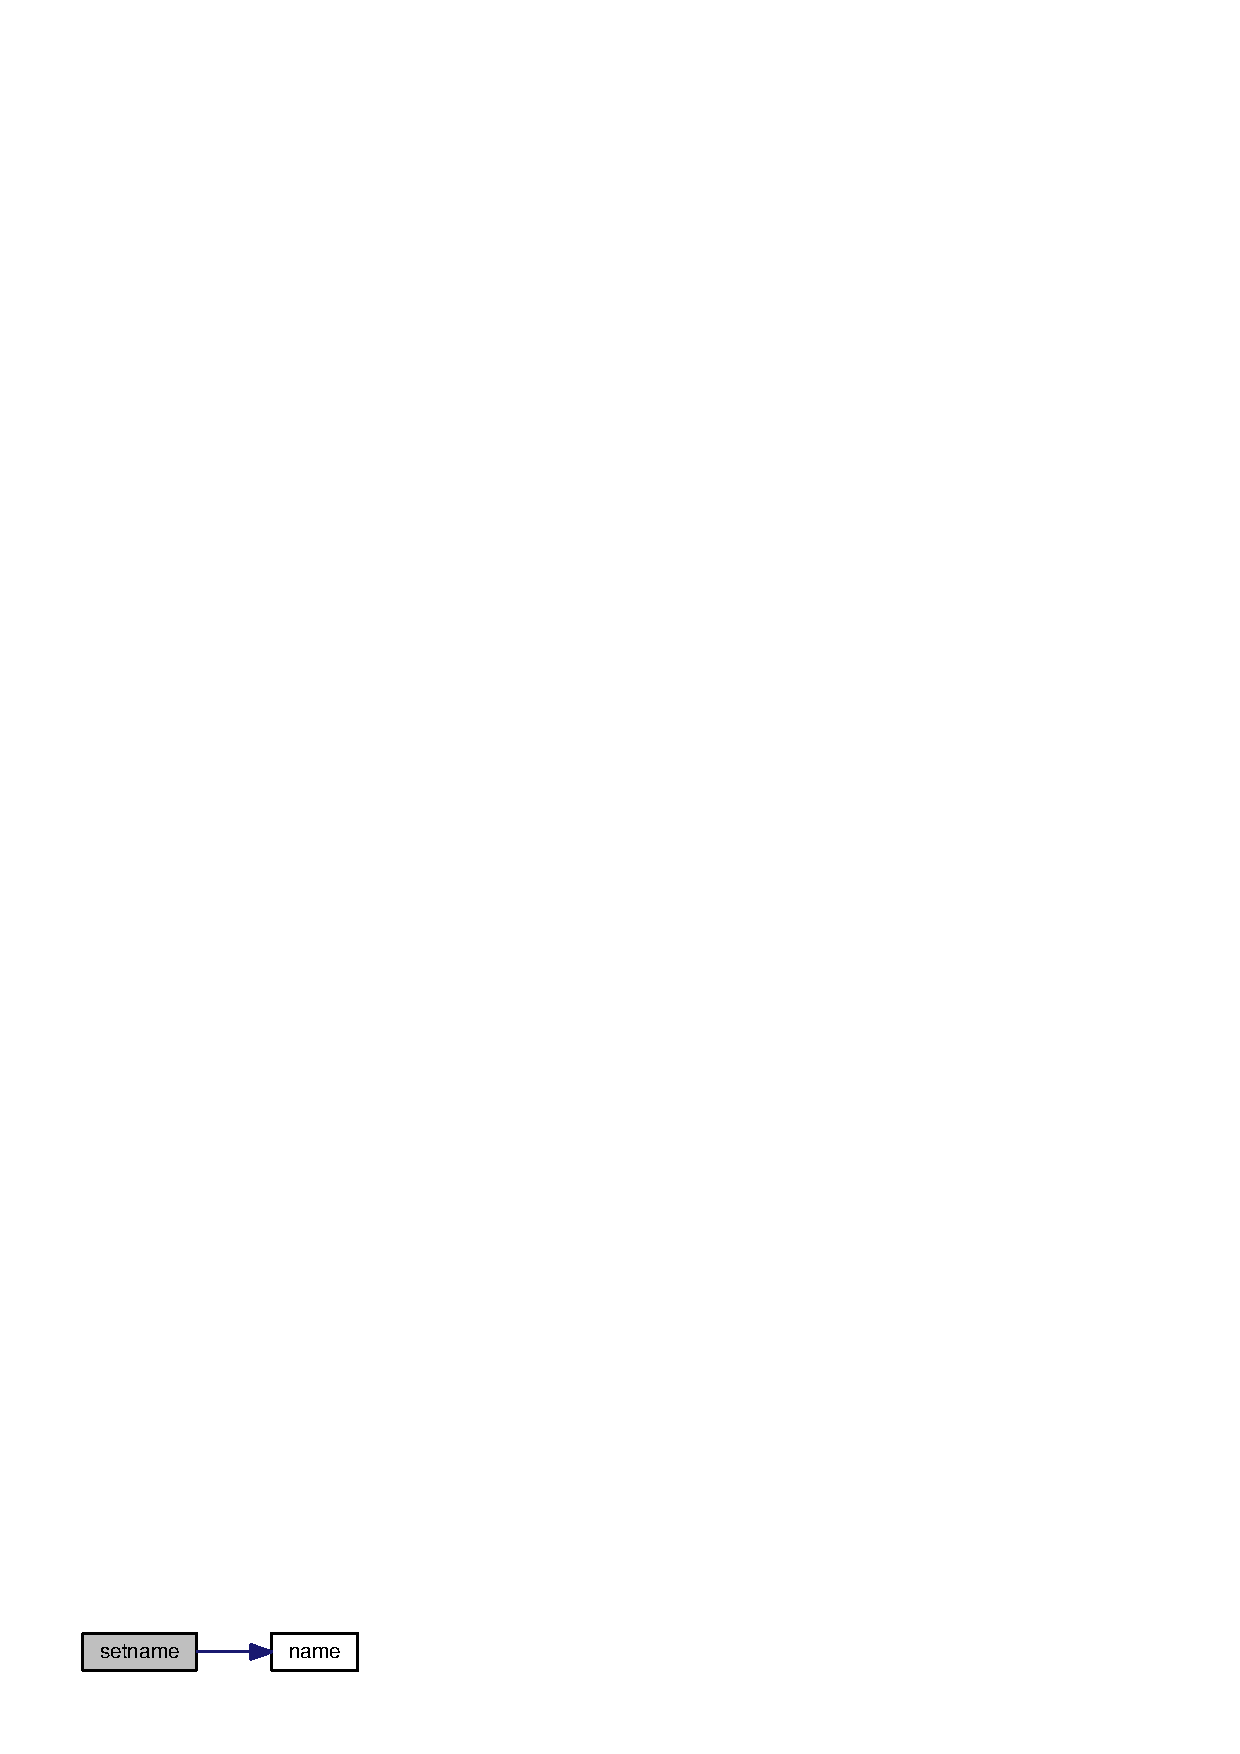
\includegraphics[width=176pt]{classorg_1_1smallfoot_1_1vw4_1_1Entity_a670f83b1f0f39a20e0fe60597032a367_cgraph}
\end{center}
\end{figure}


\index{org\+::smallfoot\+::vw4\+::\+Entity@{org\+::smallfoot\+::vw4\+::\+Entity}!vwentity@{vwentity}}
\index{vwentity@{vwentity}!org\+::smallfoot\+::vw4\+::\+Entity@{org\+::smallfoot\+::vw4\+::\+Entity}}
\subsubsection[{vwentity}]{\setlength{\rightskip}{0pt plus 5cm}abstract org.\+smallfoot.\+vw4.\+V\+W\+Import.\+Entity vwentity (
\begin{DoxyParamCaption}
\item[{String}]{tag}
\end{DoxyParamCaption}
)\hspace{0.3cm}{\ttfamily [abstract]}, {\ttfamily [protected]}}\label{classorg_1_1smallfoot_1_1vw4_1_1Entity_ad132dc987577f0c56ebcd762c3bddddb}


create a streamable J\+S\+O\+N entity from this one 

\begin{DoxyReturn}{Returns}
a org.\+smallfoot.\+vw4.\+V\+W\+Import.\+Entity representation of this instance 
\end{DoxyReturn}

\begin{DoxyParams}{Parameters}
{\em tag} & default tag to apply \\
\hline
\end{DoxyParams}


The documentation for this class was generated from the following file\+:\begin{DoxyCompactItemize}
\item 
java/{\bf Entity.\+java}\end{DoxyCompactItemize}

\section{Entity\+Array Class Reference}
\label{classorg_1_1smallfoot_1_1vw4_1_1EntityArray}\index{Entity\+Array@{Entity\+Array}}


An \doxyref{Entity\+Array}{p.}{classorg_1_1smallfoot_1_1vw4_1_1EntityArray} is the representation of an Array entity in the J\+S\+O\+N import for V\+W4.  




Inheritance diagram for Entity\+Array\+:\nopagebreak
\begin{figure}[H]
\begin{center}
\leavevmode
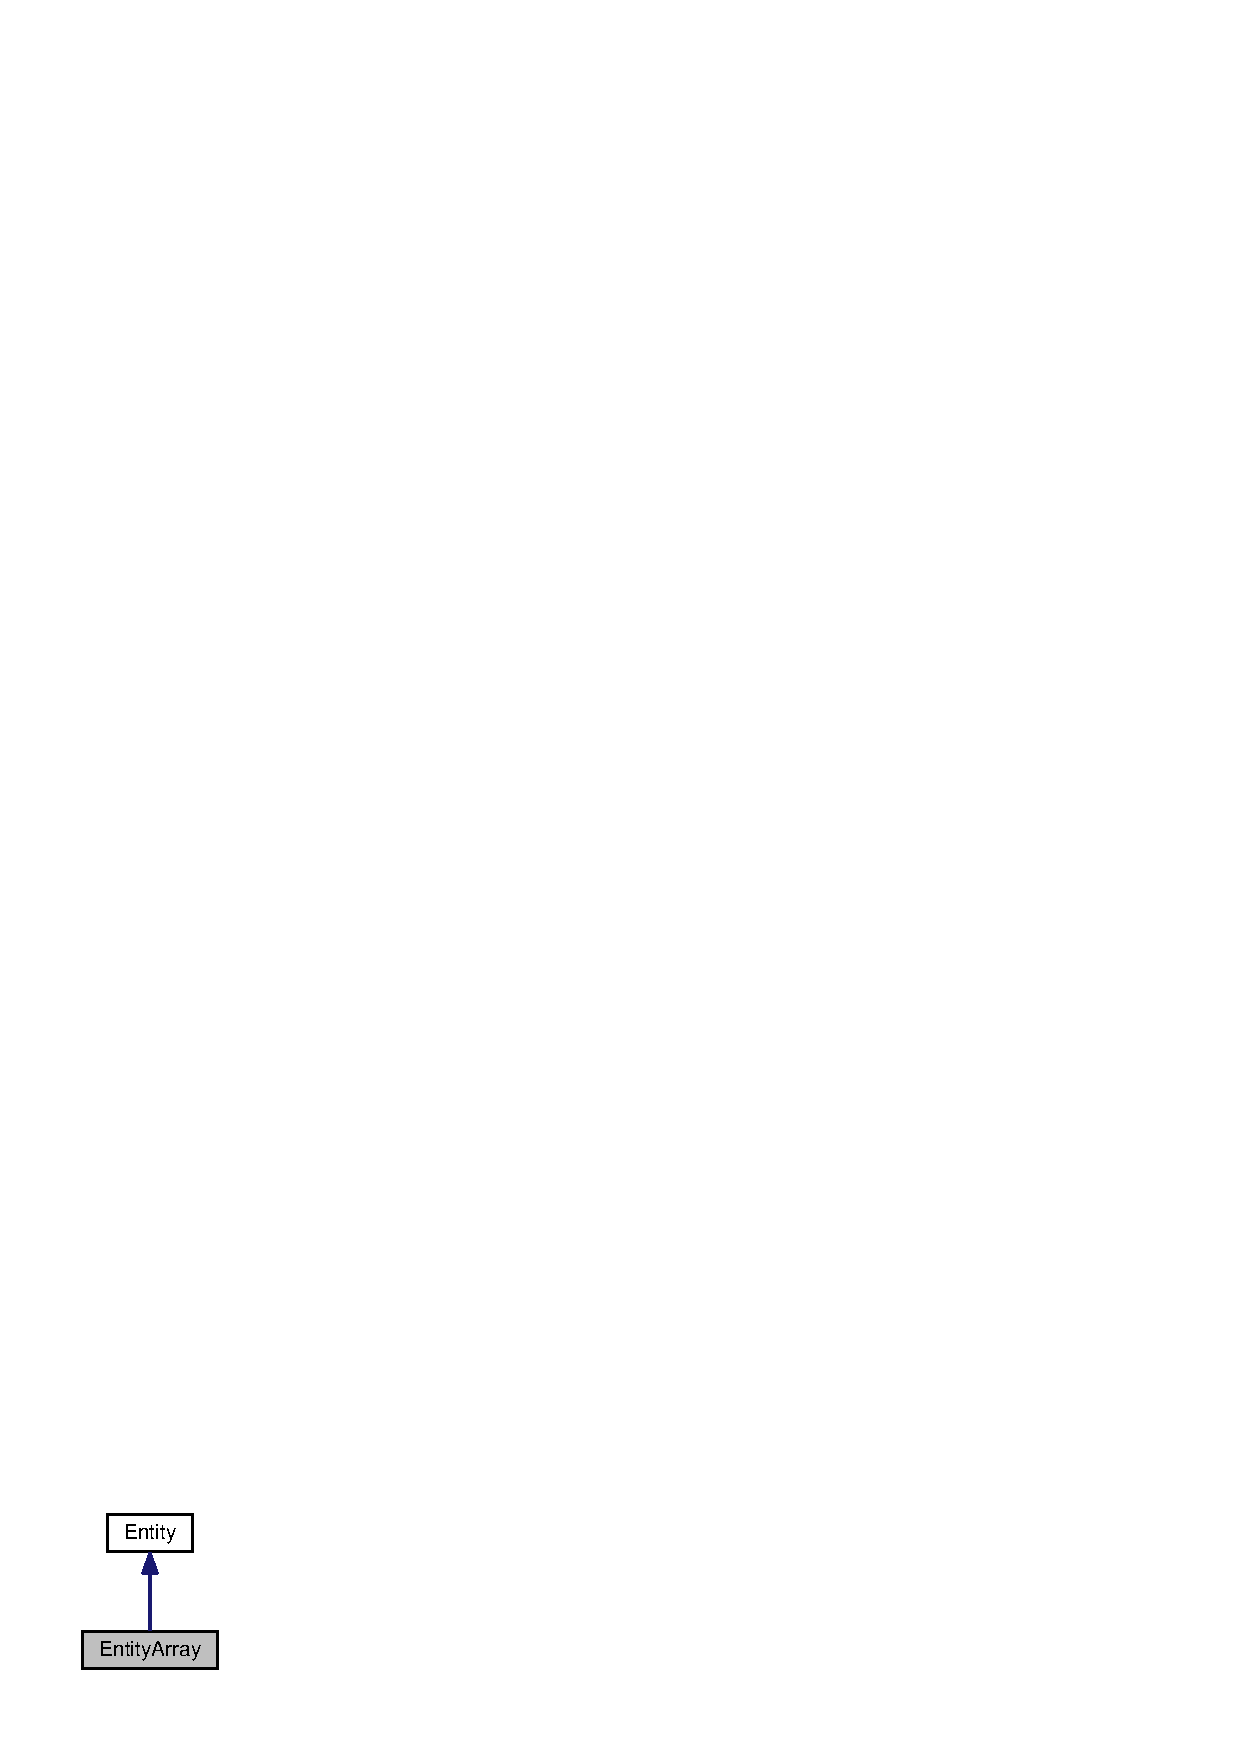
\includegraphics[width=108pt]{classorg_1_1smallfoot_1_1vw4_1_1EntityArray__inherit__graph}
\end{center}
\end{figure}


Collaboration diagram for Entity\+Array\+:\nopagebreak
\begin{figure}[H]
\begin{center}
\leavevmode
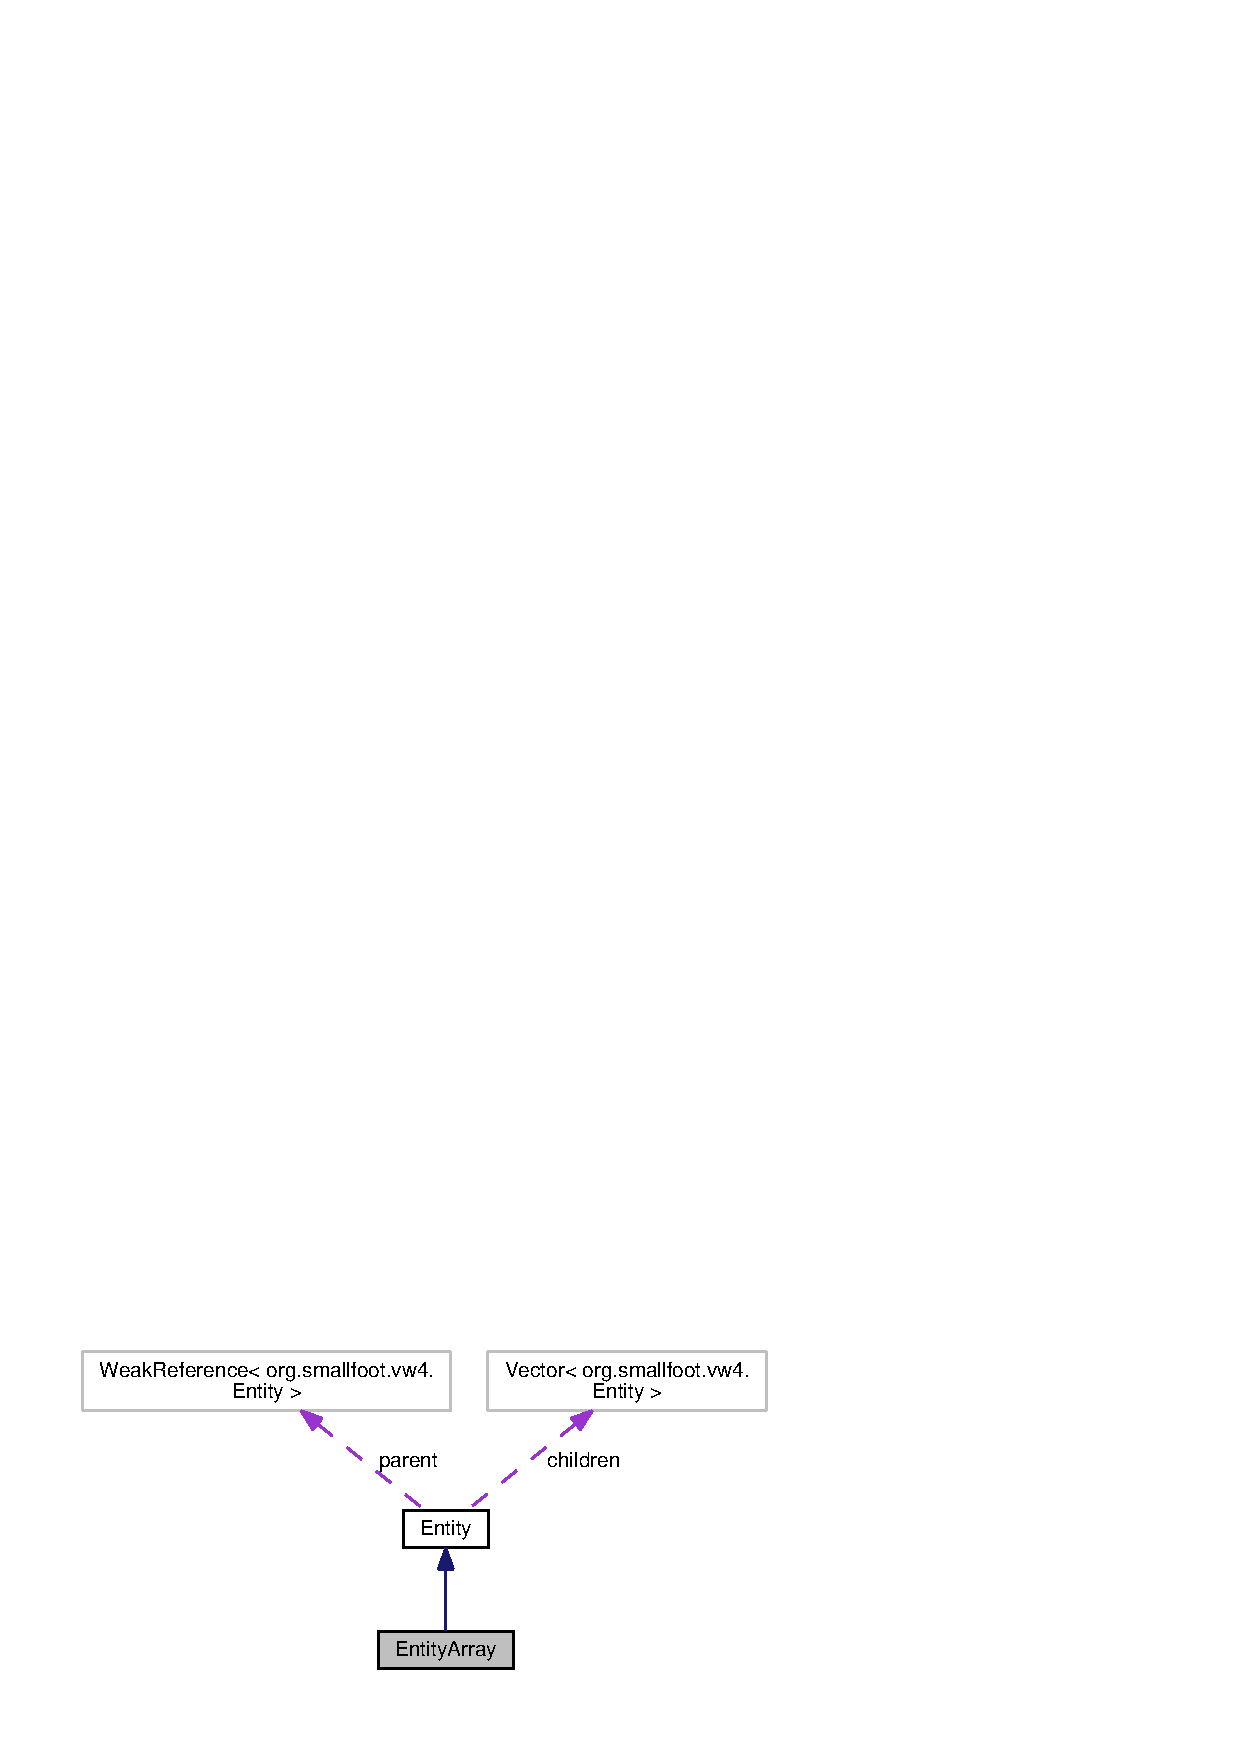
\includegraphics[width=350pt]{classorg_1_1smallfoot_1_1vw4_1_1EntityArray__coll__graph}
\end{center}
\end{figure}
\subsection*{Public Member Functions}
\begin{DoxyCompactItemize}
\item 
{\bf Entity\+Array} (String {\bf name}, {\bf Entity} e)  throws Improper\+Child\+Exception     \label{classorg_1_1smallfoot_1_1vw4_1_1EntityArray_a82720c65ff67c93dc762f047d8916488}

\begin{DoxyCompactList}\small\item\em Basic Class Constructor. \end{DoxyCompactList}\item 
{\bf Entity} {\bf new\+Parent} (String {\bf name})\label{classorg_1_1smallfoot_1_1vw4_1_1EntityArray_ae3cca685b4cef300a70d257f519a96e4}

\begin{DoxyCompactList}\small\item\em create a new \doxyref{Entity}{p.}{classorg_1_1smallfoot_1_1vw4_1_1Entity} of the correct class to be a parent of this one \end{DoxyCompactList}\end{DoxyCompactItemize}
\subsection*{Protected Member Functions}
\begin{DoxyCompactItemize}
\item 
boolean {\bf can\+Be\+Child} ({\bf Entity} e)
\begin{DoxyCompactList}\small\item\em whether a given entity can be this entity's child \end{DoxyCompactList}\item 
org.\+smallfoot.\+vw4.\+V\+W\+Import.\+Entity {\bf vwentity} (String tag)
\begin{DoxyCompactList}\small\item\em create a streamable J\+S\+O\+N entity from this one \end{DoxyCompactList}\end{DoxyCompactItemize}
\subsection*{Additional Inherited Members}


\subsection{Detailed Description}
An \doxyref{Entity\+Array}{p.}{classorg_1_1smallfoot_1_1vw4_1_1EntityArray} is the representation of an Array entity in the J\+S\+O\+N import for V\+W4. 

Be very careful\+: there is an \doxyref{Entity}{p.}{classorg_1_1smallfoot_1_1vw4_1_1Entity}, and a V\+W\+Import\+::\+Entity 

Definition at line 44 of file Entity\+Array.\+java.



\subsection{Member Function Documentation}
\index{org\+::smallfoot\+::vw4\+::\+Entity\+Array@{org\+::smallfoot\+::vw4\+::\+Entity\+Array}!can\+Be\+Child@{can\+Be\+Child}}
\index{can\+Be\+Child@{can\+Be\+Child}!org\+::smallfoot\+::vw4\+::\+Entity\+Array@{org\+::smallfoot\+::vw4\+::\+Entity\+Array}}
\subsubsection[{can\+Be\+Child}]{\setlength{\rightskip}{0pt plus 5cm}boolean can\+Be\+Child (
\begin{DoxyParamCaption}
\item[{{\bf Entity}}]{e}
\end{DoxyParamCaption}
)\hspace{0.3cm}{\ttfamily [inline]}, {\ttfamily [protected]}}\label{classorg_1_1smallfoot_1_1vw4_1_1EntityArray_a5a51654ce8be38d5f06faa182cb70e61}


whether a given entity can be this entity's child 

\begin{DoxyReturn}{Returns}
true if accepted, false if refused 
\end{DoxyReturn}

\begin{DoxyParams}{Parameters}
{\em e} & entity to check for possible descendent-\/hood \\
\hline
\end{DoxyParams}


Definition at line 55 of file Entity\+Array.\+java.

\index{org\+::smallfoot\+::vw4\+::\+Entity\+Array@{org\+::smallfoot\+::vw4\+::\+Entity\+Array}!vwentity@{vwentity}}
\index{vwentity@{vwentity}!org\+::smallfoot\+::vw4\+::\+Entity\+Array@{org\+::smallfoot\+::vw4\+::\+Entity\+Array}}
\subsubsection[{vwentity}]{\setlength{\rightskip}{0pt plus 5cm}org.\+smallfoot.\+vw4.\+V\+W\+Import.\+Entity vwentity (
\begin{DoxyParamCaption}
\item[{String}]{tag}
\end{DoxyParamCaption}
)\hspace{0.3cm}{\ttfamily [inline]}, {\ttfamily [protected]}}\label{classorg_1_1smallfoot_1_1vw4_1_1EntityArray_a1d6bf85ddf0a9382cfa4f82dd3063473}


create a streamable J\+S\+O\+N entity from this one 

\begin{DoxyReturn}{Returns}
a org.\+smallfoot.\+vw4.\+V\+W\+Import.\+Entity representation of this instance 
\end{DoxyReturn}

\begin{DoxyParams}{Parameters}
{\em tag} & default tag to apply \\
\hline
\end{DoxyParams}


Definition at line 61 of file Entity\+Array.\+java.



References Entity.\+children(), Entity.\+description(), and Entity.\+name().



Here is the call graph for this function\+:\nopagebreak
\begin{figure}[H]
\begin{center}
\leavevmode
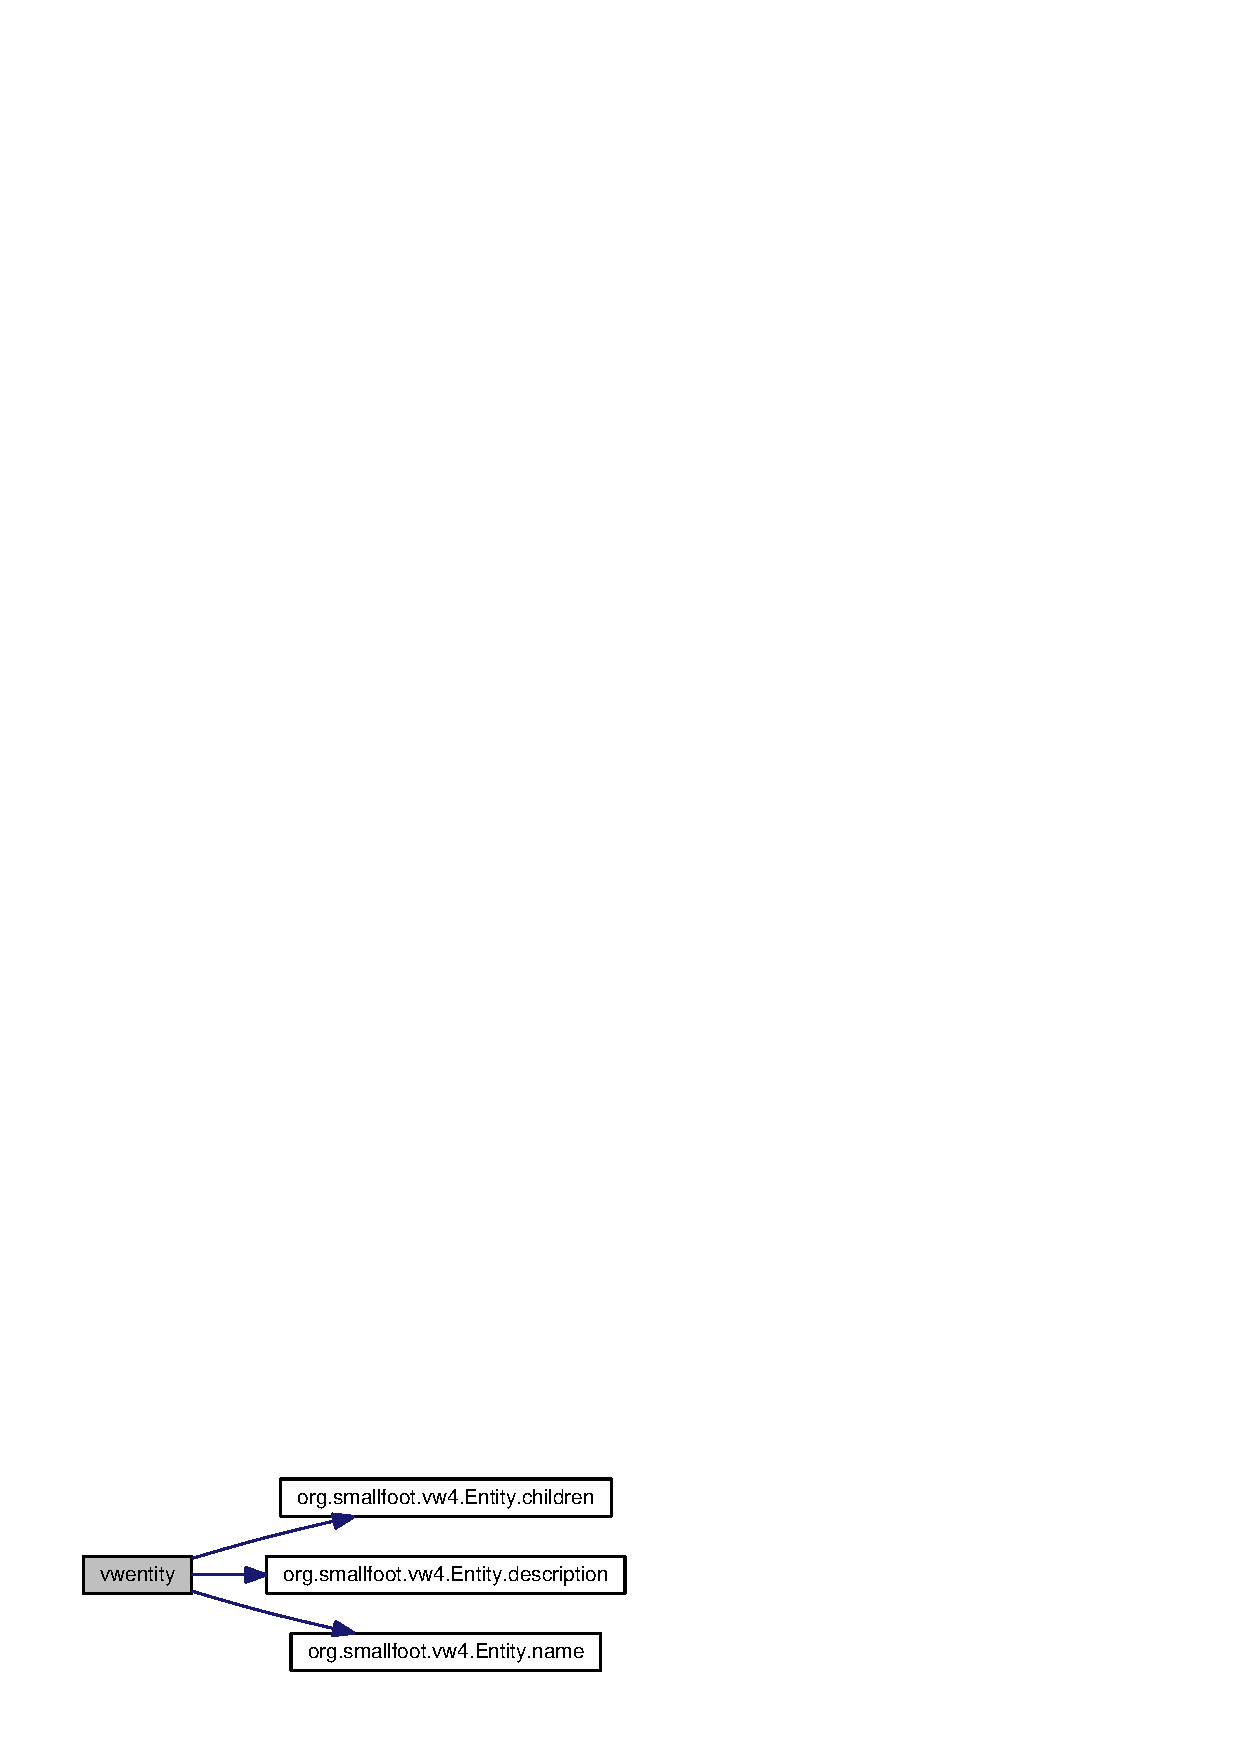
\includegraphics[width=304pt]{classorg_1_1smallfoot_1_1vw4_1_1EntityArray_a1d6bf85ddf0a9382cfa4f82dd3063473_cgraph}
\end{center}
\end{figure}




The documentation for this class was generated from the following file\+:\begin{DoxyCompactItemize}
\item 
java/{\bf Entity\+Array.\+java}\end{DoxyCompactItemize}

\section{Entity\+F\+A Class Reference}
\label{classorg_1_1smallfoot_1_1vw4_1_1EntityFA}\index{Entity\+F\+A@{Entity\+F\+A}}


An \doxyref{Entity\+F\+A}{p.}{classorg_1_1smallfoot_1_1vw4_1_1EntityFA} is the representation of an Storage F\+A entity in the J\+S\+O\+N import for V\+W4.  




Inheritance diagram for Entity\+F\+A\+:\nopagebreak
\begin{figure}[H]
\begin{center}
\leavevmode
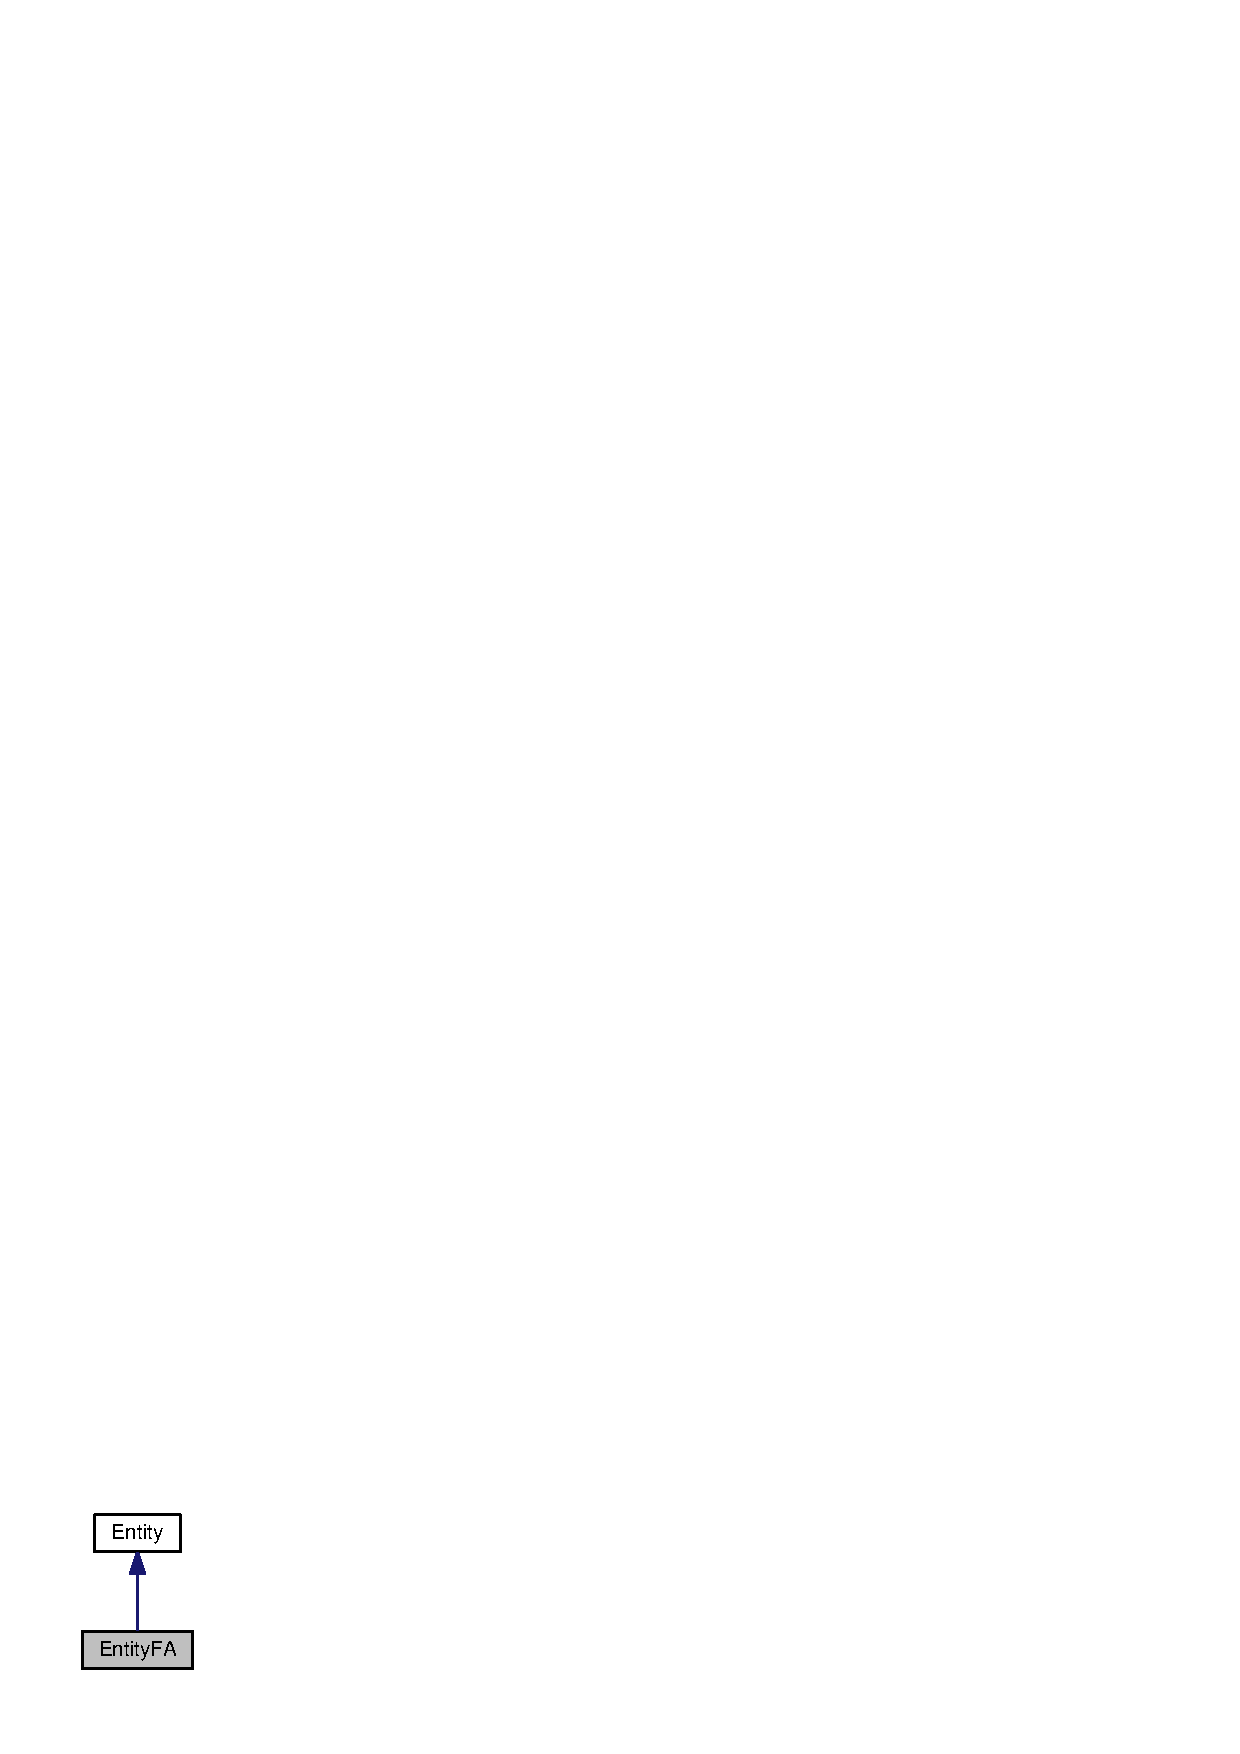
\includegraphics[width=96pt]{classorg_1_1smallfoot_1_1vw4_1_1EntityFA__inherit__graph}
\end{center}
\end{figure}


Collaboration diagram for Entity\+F\+A\+:\nopagebreak
\begin{figure}[H]
\begin{center}
\leavevmode
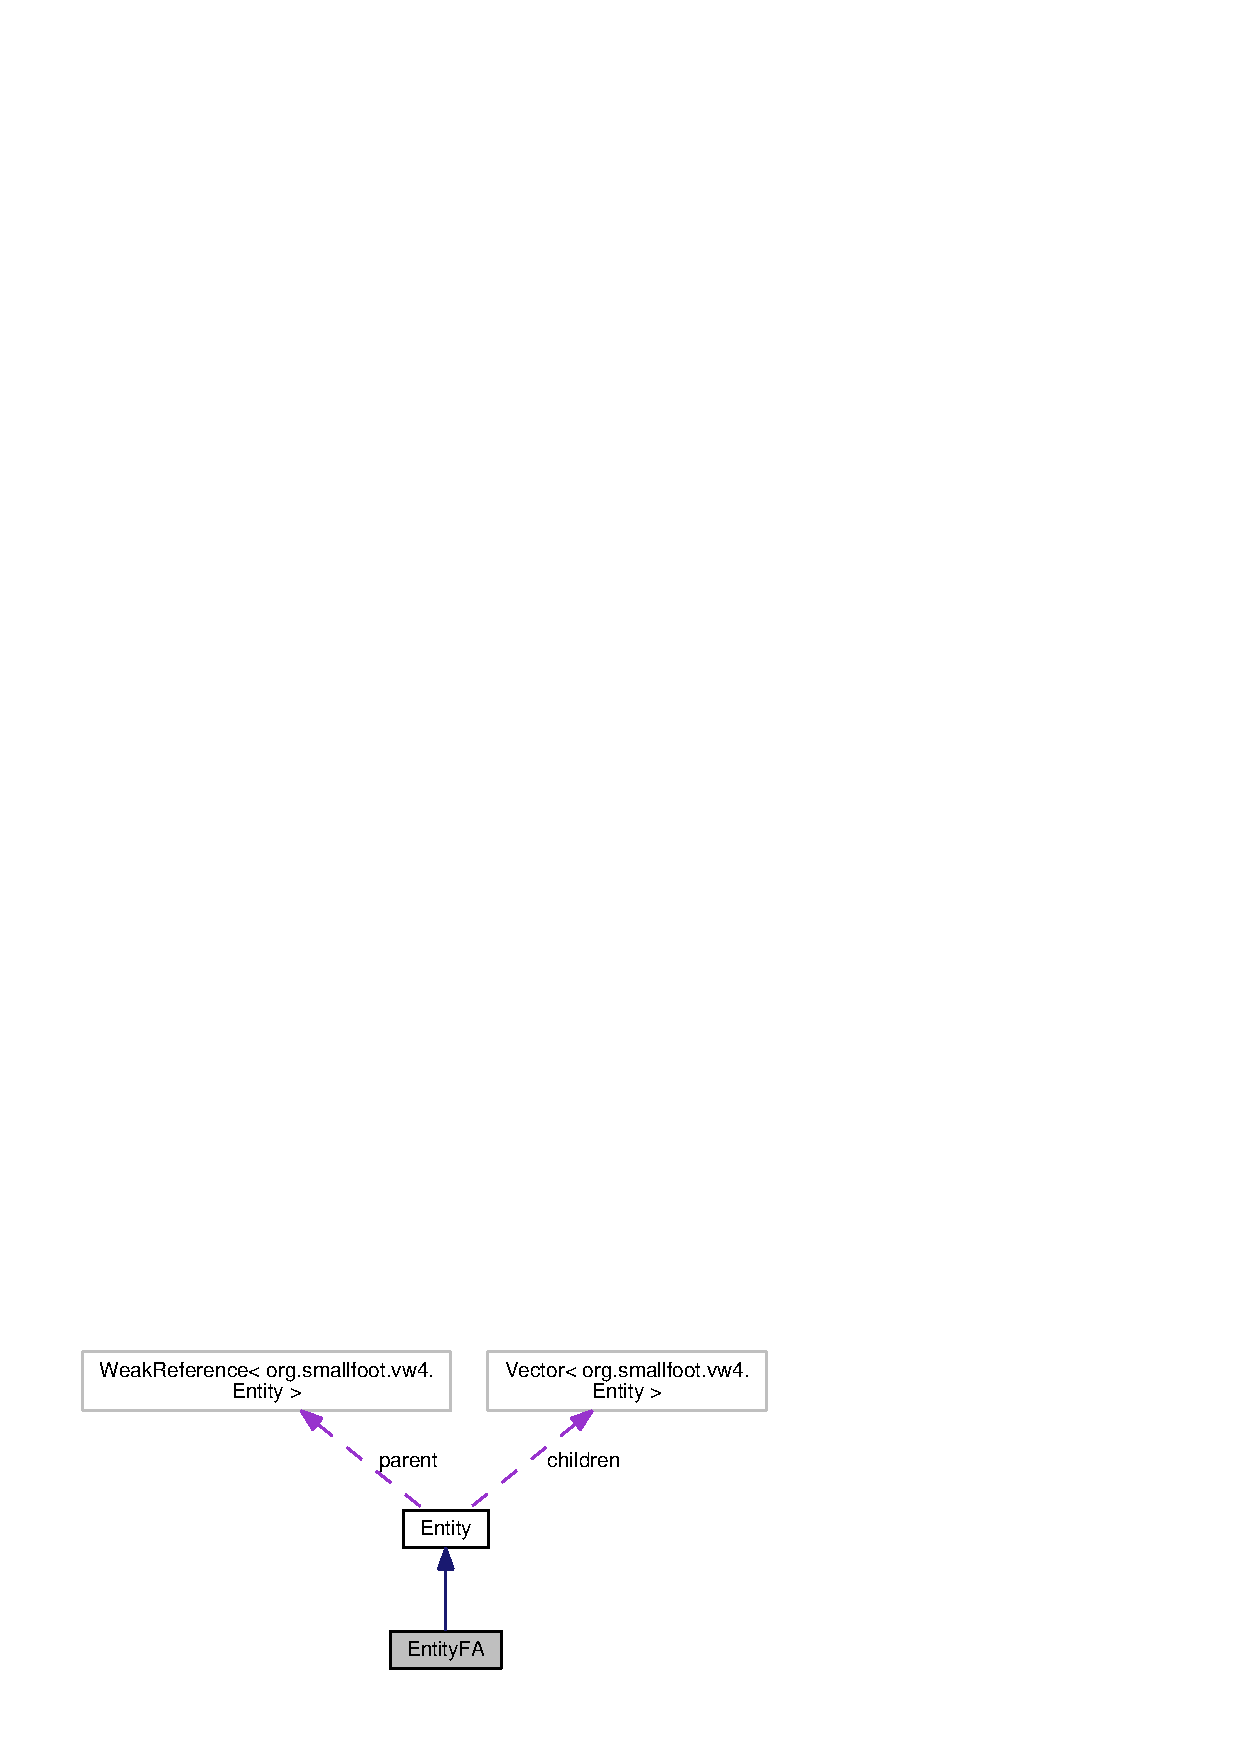
\includegraphics[width=350pt]{classorg_1_1smallfoot_1_1vw4_1_1EntityFA__coll__graph}
\end{center}
\end{figure}
\subsection*{Public Member Functions}
\begin{DoxyCompactItemize}
\item 
{\bf Entity\+F\+A} (String {\bf name}, String {\bf wwn})\label{classorg_1_1smallfoot_1_1vw4_1_1EntityFA_aee1f13fcac25df5320b16ca060ad99dd}

\begin{DoxyCompactList}\small\item\em Class Constructor with no initial child. \end{DoxyCompactList}\item 
String {\bf wwn} ()
\end{DoxyCompactItemize}
\subsection*{Protected Member Functions}
\begin{DoxyCompactItemize}
\item 
boolean {\bf can\+Be\+Child} ({\bf Entity} e)
\item 
org.\+smallfoot.\+vw4.\+V\+W\+Import.\+Entity {\bf vwentity} (String tag)
\begin{DoxyCompactList}\small\item\em create a streamable J\+S\+O\+N entity from this one \end{DoxyCompactList}\end{DoxyCompactItemize}
\subsection*{Protected Attributes}
\begin{DoxyCompactItemize}
\item 
String {\bf wwn}\label{classorg_1_1smallfoot_1_1vw4_1_1EntityFA_ab07f595ad2e4da7c53cd29f435f5bb3c}

\begin{DoxyCompactList}\small\item\em the unique W\+W\+P\+N of the hba \end{DoxyCompactList}\end{DoxyCompactItemize}


\subsection{Detailed Description}
An \doxyref{Entity\+F\+A}{p.}{classorg_1_1smallfoot_1_1vw4_1_1EntityFA} is the representation of an Storage F\+A entity in the J\+S\+O\+N import for V\+W4. 

Be very careful\+: there is an \doxyref{Entity}{p.}{classorg_1_1smallfoot_1_1vw4_1_1Entity}, and a V\+W\+Import\+::\+Entity 

Definition at line 44 of file Entity\+F\+A.\+java.



\subsection{Member Function Documentation}
\index{org\+::smallfoot\+::vw4\+::\+Entity\+F\+A@{org\+::smallfoot\+::vw4\+::\+Entity\+F\+A}!can\+Be\+Child@{can\+Be\+Child}}
\index{can\+Be\+Child@{can\+Be\+Child}!org\+::smallfoot\+::vw4\+::\+Entity\+F\+A@{org\+::smallfoot\+::vw4\+::\+Entity\+F\+A}}
\subsubsection[{can\+Be\+Child}]{\setlength{\rightskip}{0pt plus 5cm}boolean can\+Be\+Child (
\begin{DoxyParamCaption}
\item[{{\bf Entity}}]{e}
\end{DoxyParamCaption}
)\hspace{0.3cm}{\ttfamily [inline]}, {\ttfamily [protected]}}\label{classorg_1_1smallfoot_1_1vw4_1_1EntityFA_a5a51654ce8be38d5f06faa182cb70e61}
$<$ this entity has no children so this method will always be false 

Definition at line 62 of file Entity\+F\+A.\+java.

\index{org\+::smallfoot\+::vw4\+::\+Entity\+F\+A@{org\+::smallfoot\+::vw4\+::\+Entity\+F\+A}!vwentity@{vwentity}}
\index{vwentity@{vwentity}!org\+::smallfoot\+::vw4\+::\+Entity\+F\+A@{org\+::smallfoot\+::vw4\+::\+Entity\+F\+A}}
\subsubsection[{vwentity}]{\setlength{\rightskip}{0pt plus 5cm}org.\+smallfoot.\+vw4.\+V\+W\+Import.\+Entity vwentity (
\begin{DoxyParamCaption}
\item[{String}]{tag}
\end{DoxyParamCaption}
)\hspace{0.3cm}{\ttfamily [inline]}, {\ttfamily [protected]}}\label{classorg_1_1smallfoot_1_1vw4_1_1EntityFA_a1d6bf85ddf0a9382cfa4f82dd3063473}


create a streamable J\+S\+O\+N entity from this one 

\begin{DoxyReturn}{Returns}
a org.\+smallfoot.\+vw4.\+V\+W\+Import.\+Entity representation of this instance 
\end{DoxyReturn}

\begin{DoxyParams}{Parameters}
{\em tag} & default tag to apply \\
\hline
\end{DoxyParams}


Definition at line 68 of file Entity\+F\+A.\+java.



References Entity.\+description(), and Entity.\+name().



Here is the call graph for this function\+:\nopagebreak
\begin{figure}[H]
\begin{center}
\leavevmode
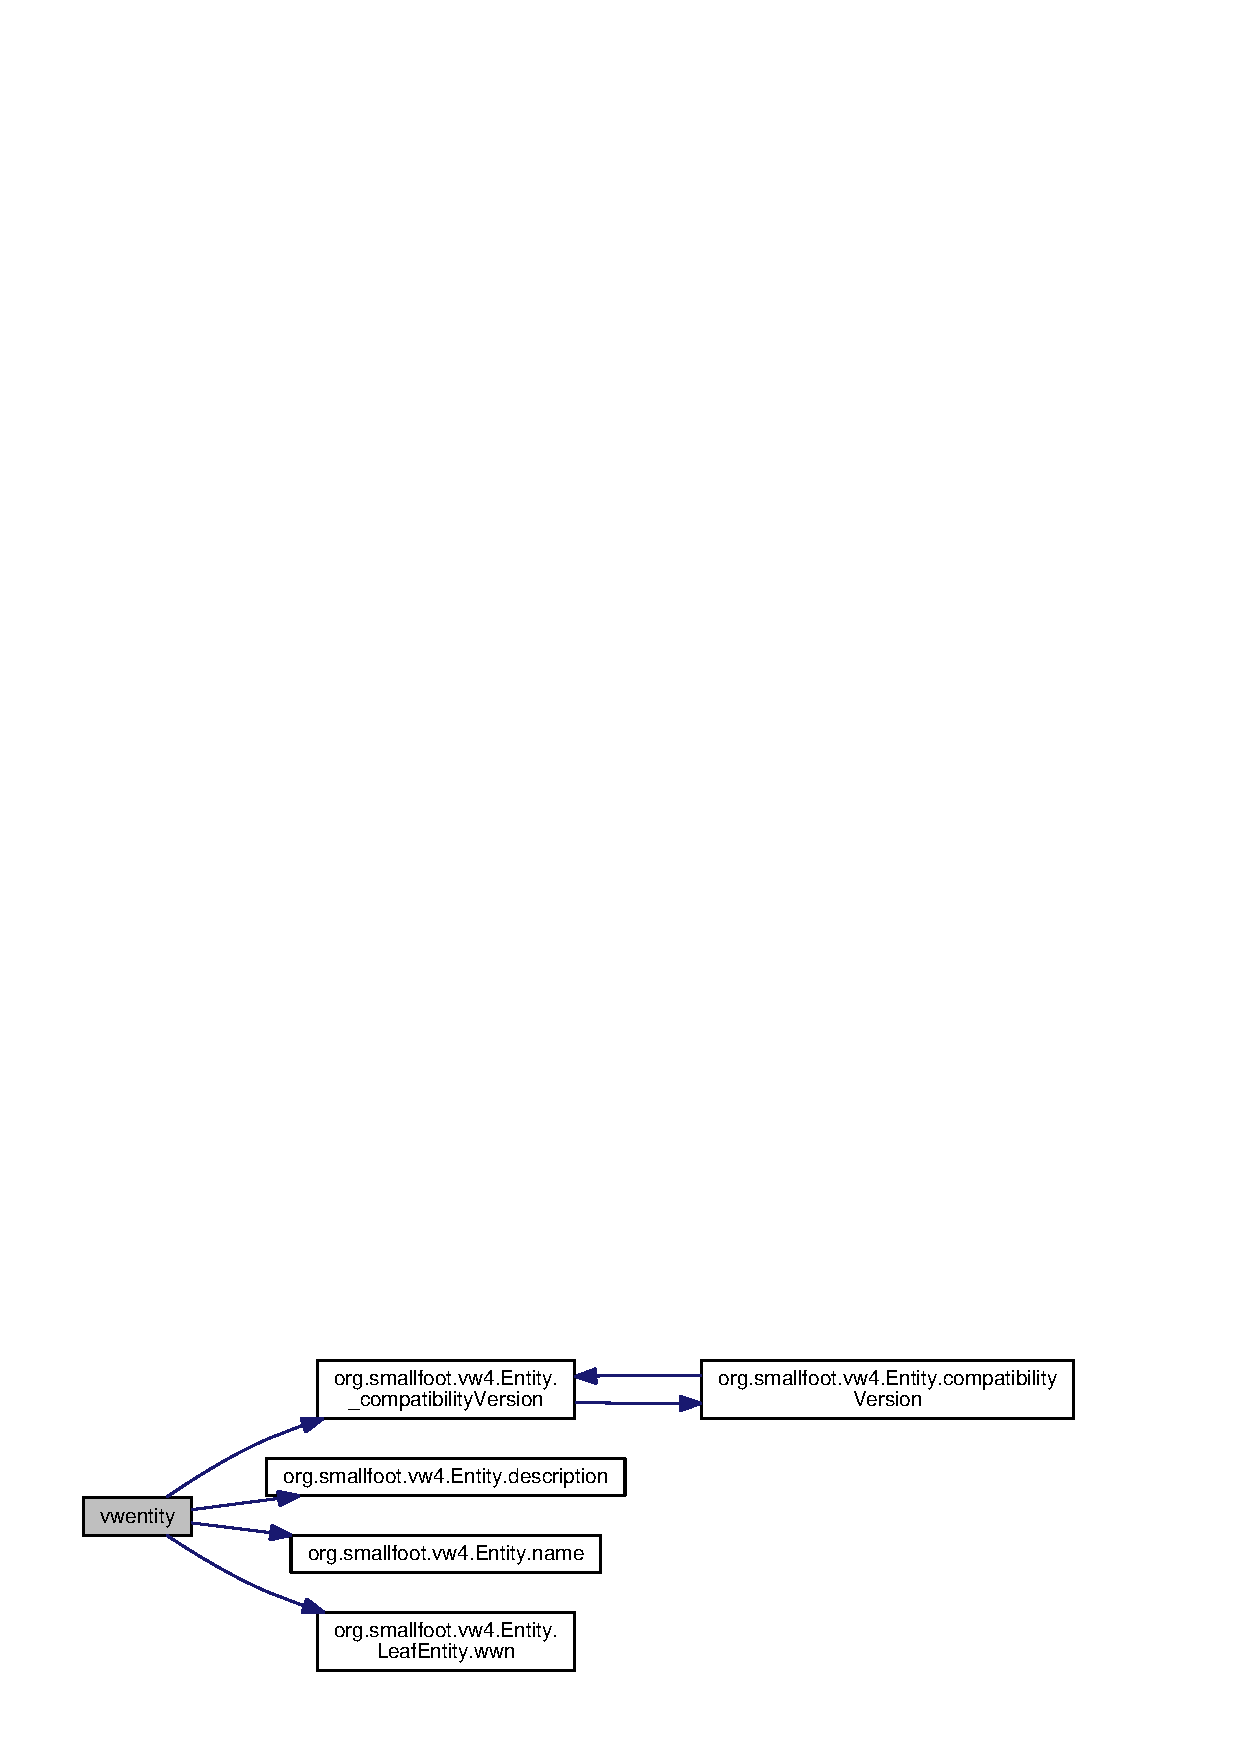
\includegraphics[width=304pt]{classorg_1_1smallfoot_1_1vw4_1_1EntityFA_a1d6bf85ddf0a9382cfa4f82dd3063473_cgraph}
\end{center}
\end{figure}


\index{org\+::smallfoot\+::vw4\+::\+Entity\+F\+A@{org\+::smallfoot\+::vw4\+::\+Entity\+F\+A}!wwn@{wwn}}
\index{wwn@{wwn}!org\+::smallfoot\+::vw4\+::\+Entity\+F\+A@{org\+::smallfoot\+::vw4\+::\+Entity\+F\+A}}
\subsubsection[{wwn}]{\setlength{\rightskip}{0pt plus 5cm}String wwn (
\begin{DoxyParamCaption}
{}
\end{DoxyParamCaption}
)\hspace{0.3cm}{\ttfamily [inline]}}\label{classorg_1_1smallfoot_1_1vw4_1_1EntityFA_aa0f20764b2a9bea375e9507de63cb42b}
$<$ getter 

Definition at line 48 of file Entity\+F\+A.\+java.



Referenced by Entity\+F\+A.\+Entity\+F\+A().



The documentation for this class was generated from the following file\+:\begin{DoxyCompactItemize}
\item 
java/{\bf Entity\+F\+A.\+java}\end{DoxyCompactItemize}

\section{Entity\+H\+B\+A Class Reference}
\label{classorg_1_1smallfoot_1_1vw4_1_1EntityHBA}\index{Entity\+H\+B\+A@{Entity\+H\+B\+A}}


An \doxyref{Entity\+H\+B\+A}{p.}{classorg_1_1smallfoot_1_1vw4_1_1EntityHBA} is the representation of an H\+B\+A entity in the J\+S\+O\+N import for V\+W4.  




Inheritance diagram for Entity\+H\+B\+A\+:\nopagebreak
\begin{figure}[H]
\begin{center}
\leavevmode
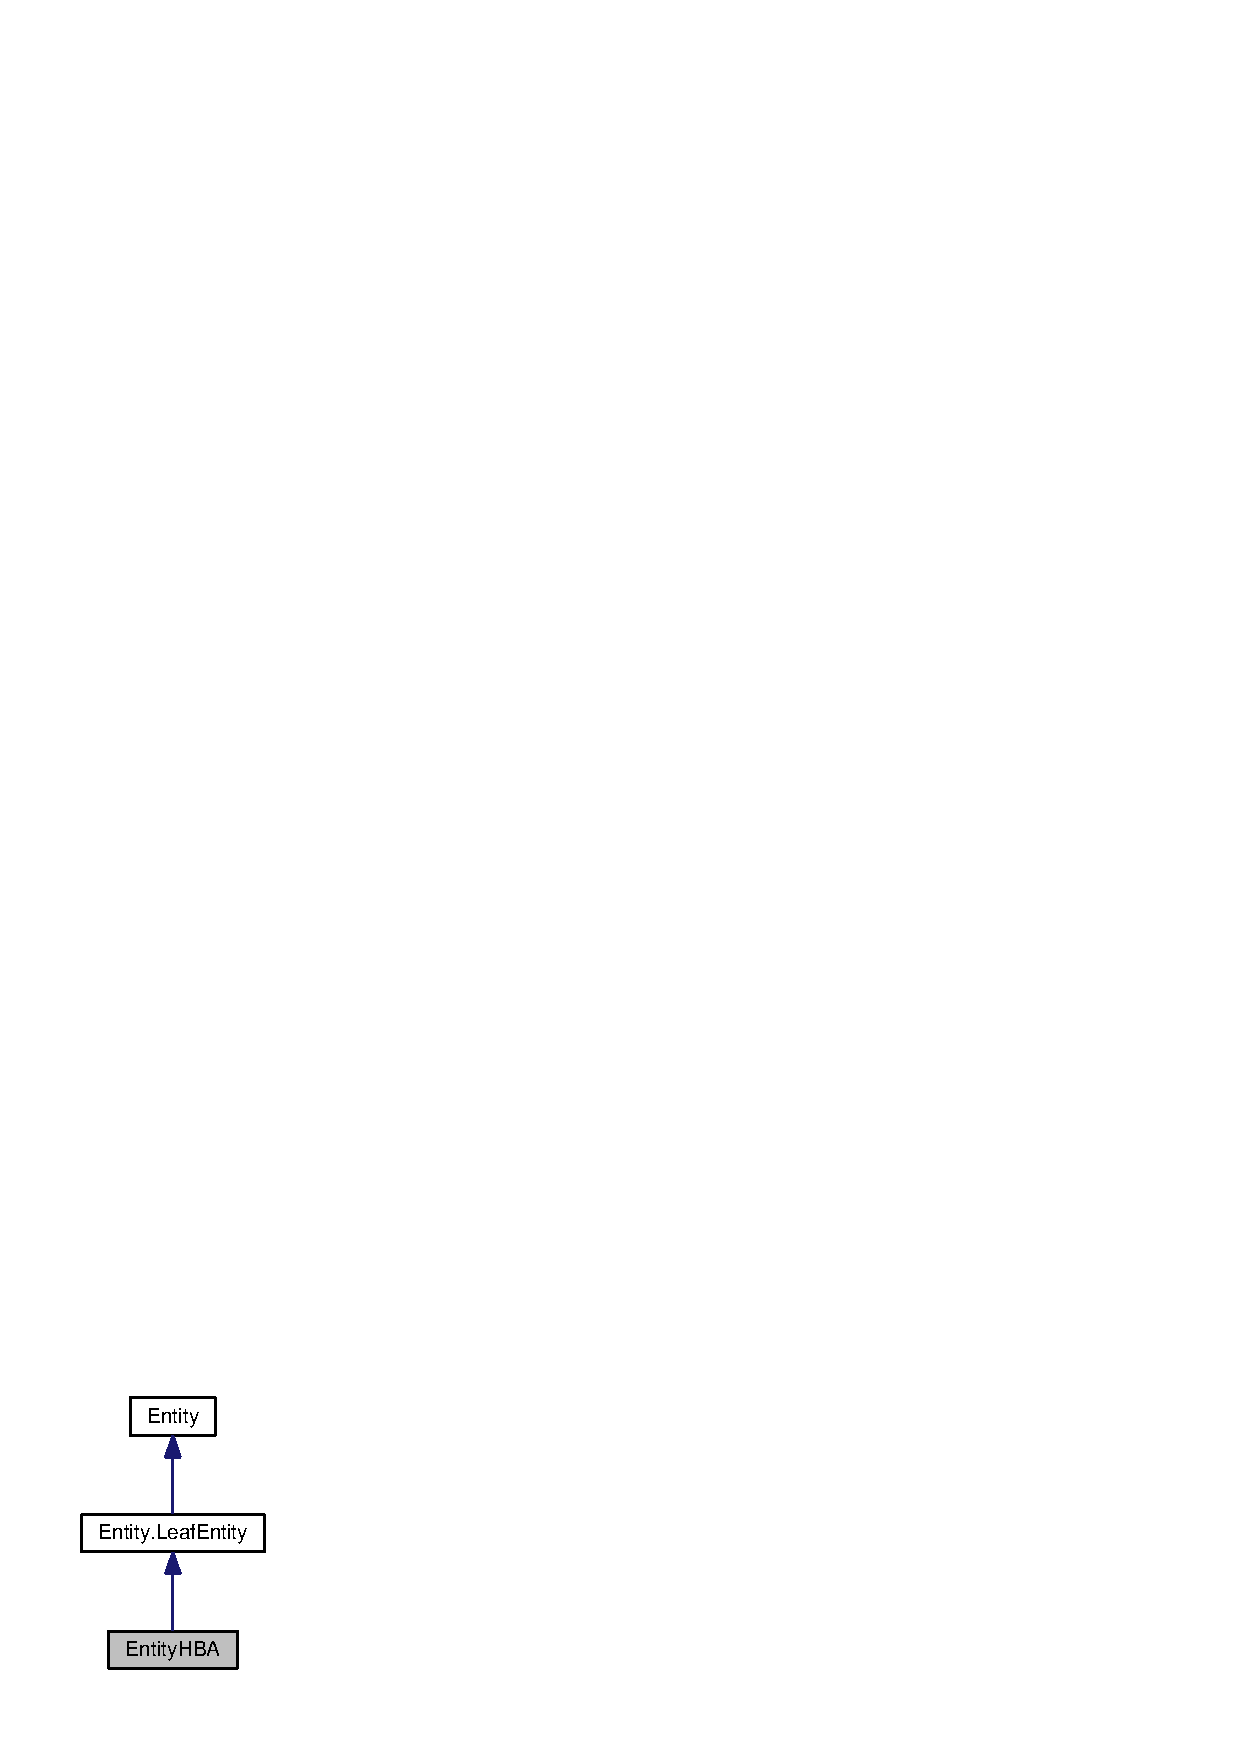
\includegraphics[width=130pt]{classorg_1_1smallfoot_1_1vw4_1_1EntityHBA__inherit__graph}
\end{center}
\end{figure}


Collaboration diagram for Entity\+H\+B\+A\+:\nopagebreak
\begin{figure}[H]
\begin{center}
\leavevmode
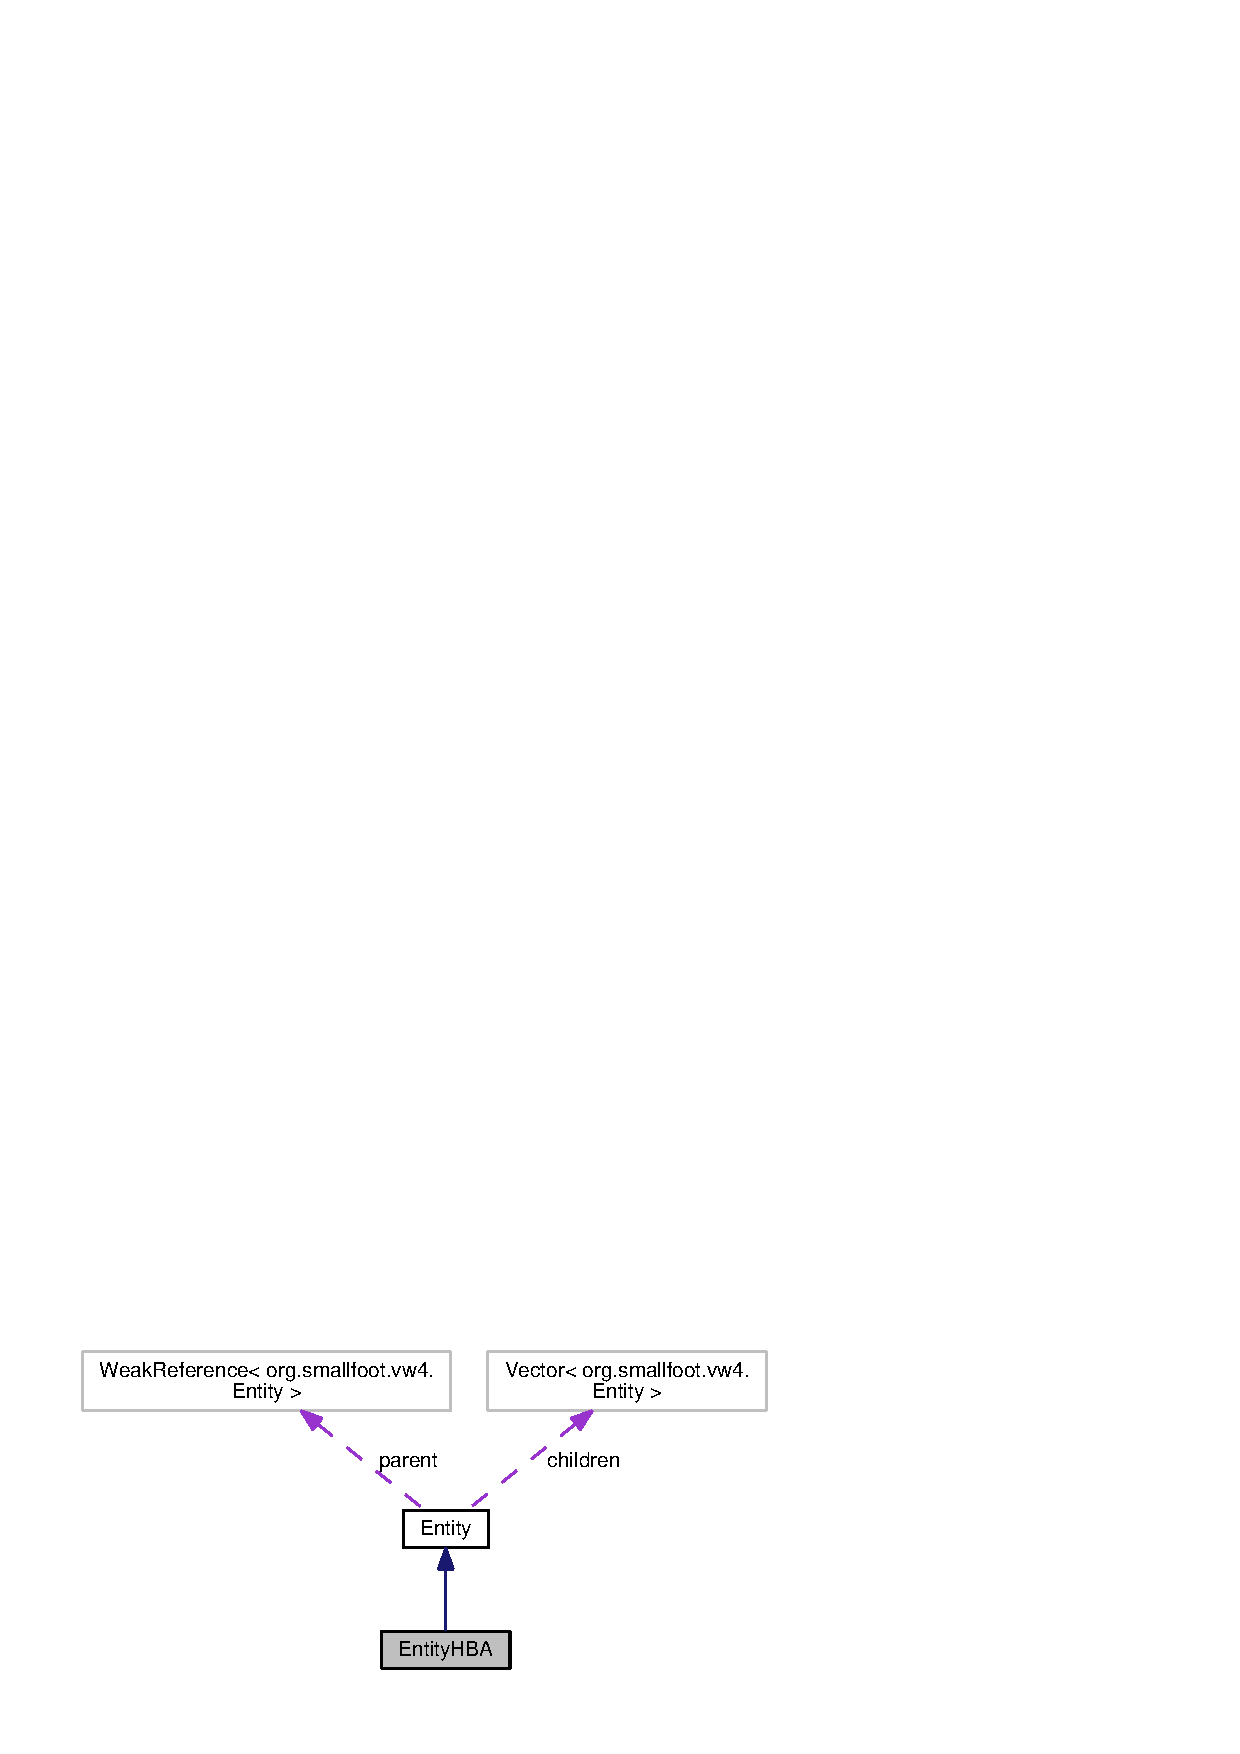
\includegraphics[width=350pt]{classorg_1_1smallfoot_1_1vw4_1_1EntityHBA__coll__graph}
\end{center}
\end{figure}
\subsection*{Public Member Functions}
\begin{DoxyCompactItemize}
\item 
{\bf Entity\+H\+B\+A} (String {\bf name}, String {\bf wwn})\label{classorg_1_1smallfoot_1_1vw4_1_1EntityHBA_a5470c9c351f0ea8dd64d612e11c7214f}

\begin{DoxyCompactList}\small\item\em Basic Class Constructor. \end{DoxyCompactList}\item 
{\bf Entity} {\bf new\+Parent} (String {\bf name})\label{classorg_1_1smallfoot_1_1vw4_1_1EntityHBA_ae3cca685b4cef300a70d257f519a96e4}

\begin{DoxyCompactList}\small\item\em create a new \doxyref{Entity}{p.}{classorg_1_1smallfoot_1_1vw4_1_1Entity} of the correct class to be a parent of this one \end{DoxyCompactList}\end{DoxyCompactItemize}
\subsection*{Protected Member Functions}
\begin{DoxyCompactItemize}
\item 
org.\+smallfoot.\+vw4.\+V\+W\+Import.\+Entity {\bf vwentity} (String tag)
\begin{DoxyCompactList}\small\item\em create a streamable J\+S\+O\+N entity from this one \end{DoxyCompactList}\end{DoxyCompactItemize}
\subsection*{Additional Inherited Members}


\subsection{Detailed Description}
An \doxyref{Entity\+H\+B\+A}{p.}{classorg_1_1smallfoot_1_1vw4_1_1EntityHBA} is the representation of an H\+B\+A entity in the J\+S\+O\+N import for V\+W4. 

Be very careful\+: there is an \doxyref{Entity}{p.}{classorg_1_1smallfoot_1_1vw4_1_1Entity}, and a V\+W\+Import\+::\+Entity 

Definition at line 44 of file Entity\+H\+B\+A.\+java.



\subsection{Member Function Documentation}
\index{org\+::smallfoot\+::vw4\+::\+Entity\+H\+B\+A@{org\+::smallfoot\+::vw4\+::\+Entity\+H\+B\+A}!vwentity@{vwentity}}
\index{vwentity@{vwentity}!org\+::smallfoot\+::vw4\+::\+Entity\+H\+B\+A@{org\+::smallfoot\+::vw4\+::\+Entity\+H\+B\+A}}
\subsubsection[{vwentity}]{\setlength{\rightskip}{0pt plus 5cm}org.\+smallfoot.\+vw4.\+V\+W\+Import.\+Entity vwentity (
\begin{DoxyParamCaption}
\item[{String}]{tag}
\end{DoxyParamCaption}
)\hspace{0.3cm}{\ttfamily [inline]}, {\ttfamily [protected]}}\label{classorg_1_1smallfoot_1_1vw4_1_1EntityHBA_a1d6bf85ddf0a9382cfa4f82dd3063473}


create a streamable J\+S\+O\+N entity from this one 

\begin{DoxyReturn}{Returns}
a org.\+smallfoot.\+vw4.\+V\+W\+Import.\+Entity representation of this instance 
\end{DoxyReturn}

\begin{DoxyParams}{Parameters}
{\em tag} & default tag to apply \\
\hline
\end{DoxyParams}


Definition at line 55 of file Entity\+H\+B\+A.\+java.



References Entity.\+description(), Entity.\+name(), and Entity.\+Leaf\+Entity.\+wwn().



Here is the call graph for this function\+:\nopagebreak
\begin{figure}[H]
\begin{center}
\leavevmode
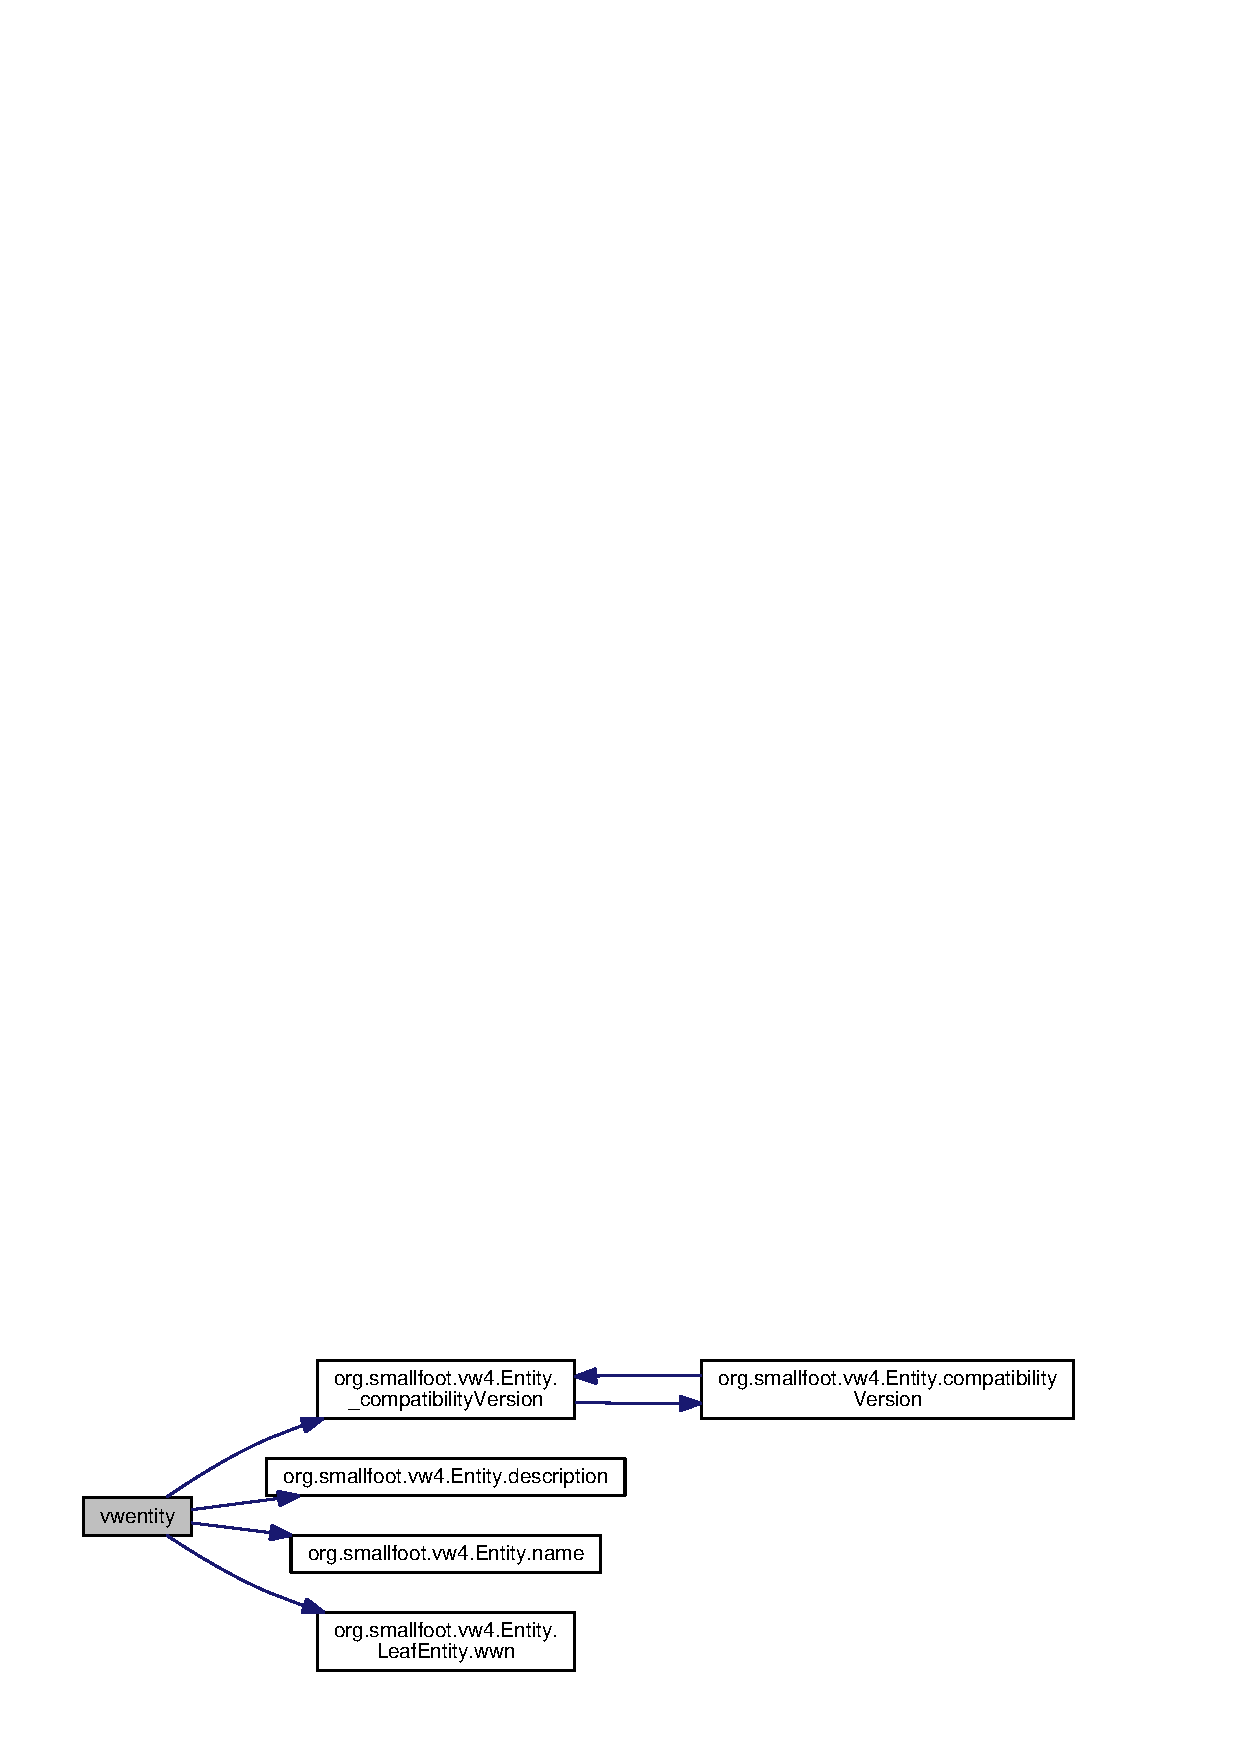
\includegraphics[width=304pt]{classorg_1_1smallfoot_1_1vw4_1_1EntityHBA_a1d6bf85ddf0a9382cfa4f82dd3063473_cgraph}
\end{center}
\end{figure}




The documentation for this class was generated from the following file\+:\begin{DoxyCompactItemize}
\item 
java/{\bf Entity\+H\+B\+A.\+java}\end{DoxyCompactItemize}

\section{Entity\+Host Class Reference}
\label{classorg_1_1smallfoot_1_1vw4_1_1EntityHost}\index{Entity\+Host@{Entity\+Host}}


An \doxyref{Entity\+Host}{p.}{classorg_1_1smallfoot_1_1vw4_1_1EntityHost} is the representation of an Host entity in the J\+S\+O\+N import for V\+W4.  




Inheritance diagram for Entity\+Host\+:\nopagebreak
\begin{figure}[H]
\begin{center}
\leavevmode
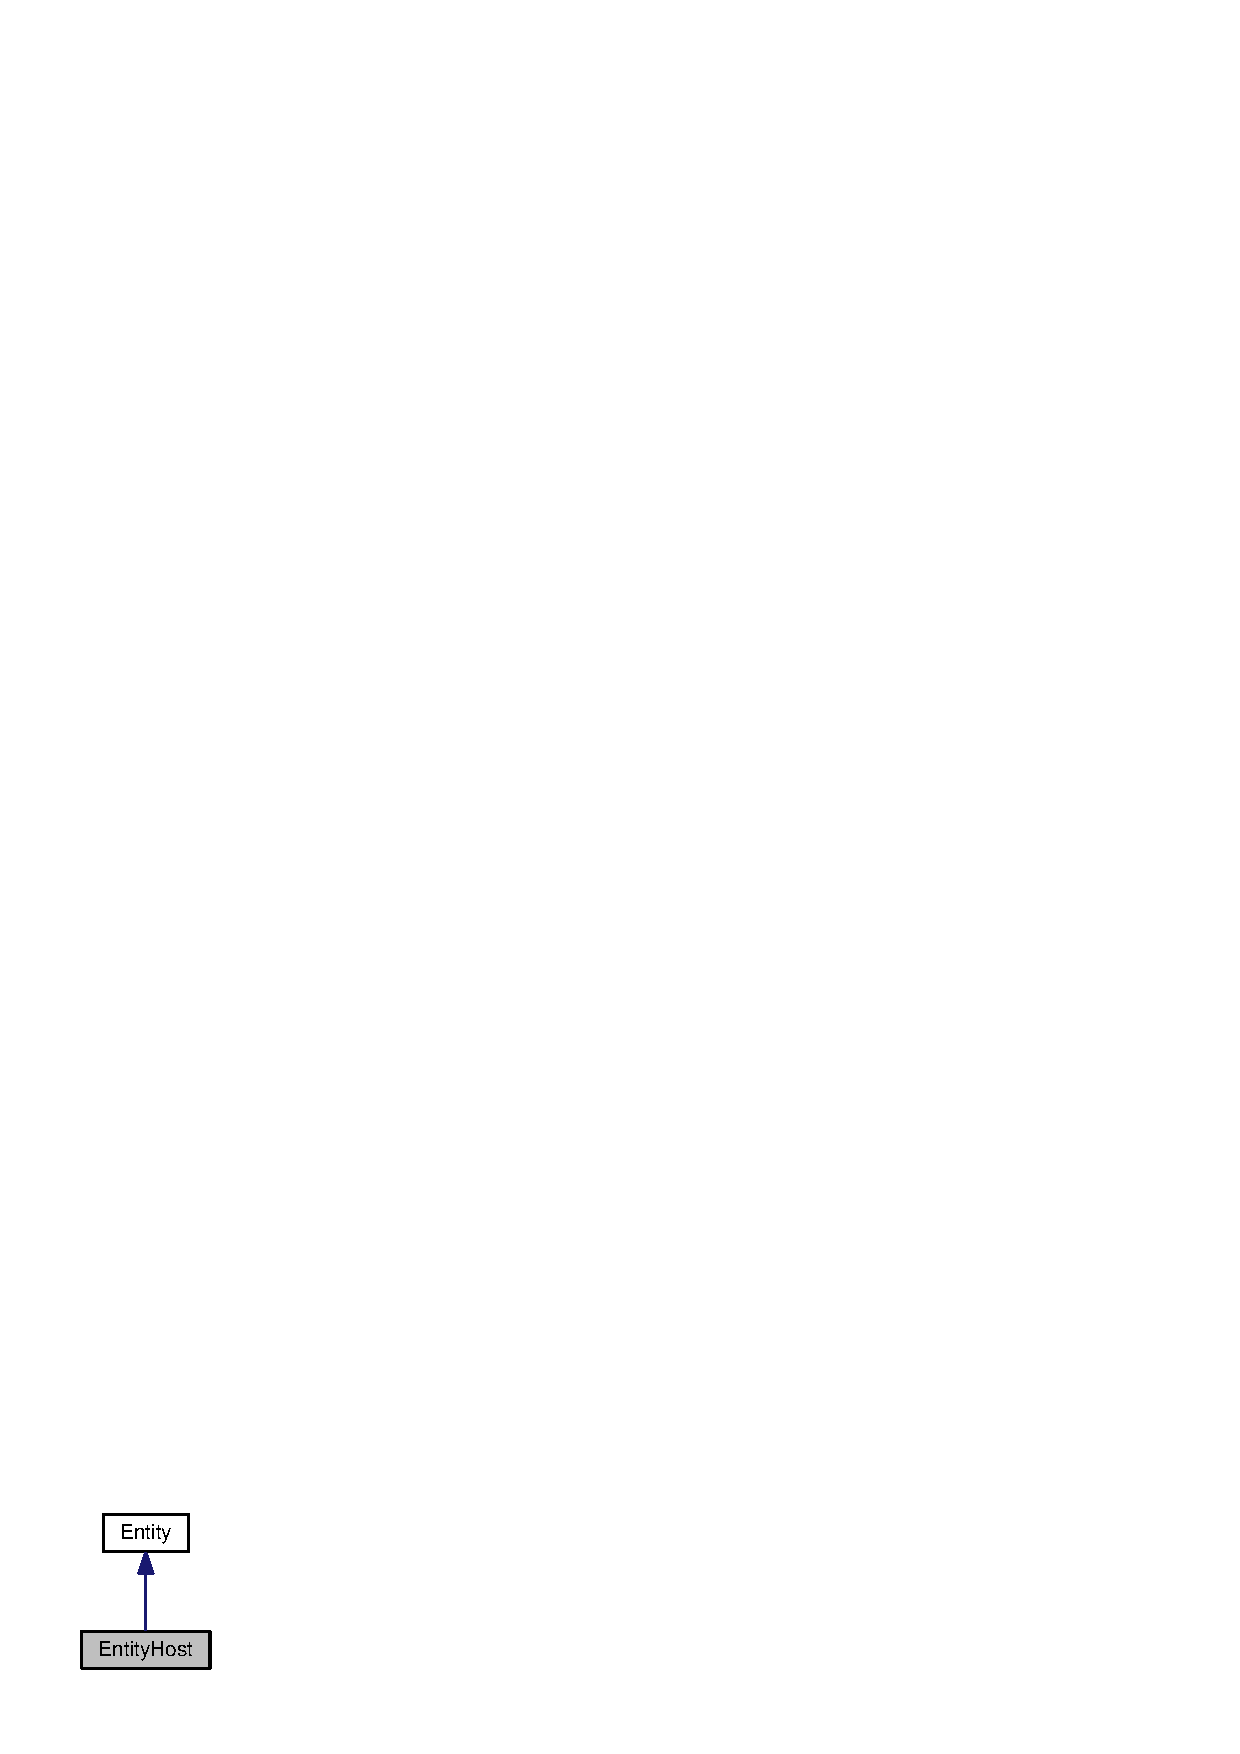
\includegraphics[width=104pt]{classorg_1_1smallfoot_1_1vw4_1_1EntityHost__inherit__graph}
\end{center}
\end{figure}


Collaboration diagram for Entity\+Host\+:\nopagebreak
\begin{figure}[H]
\begin{center}
\leavevmode
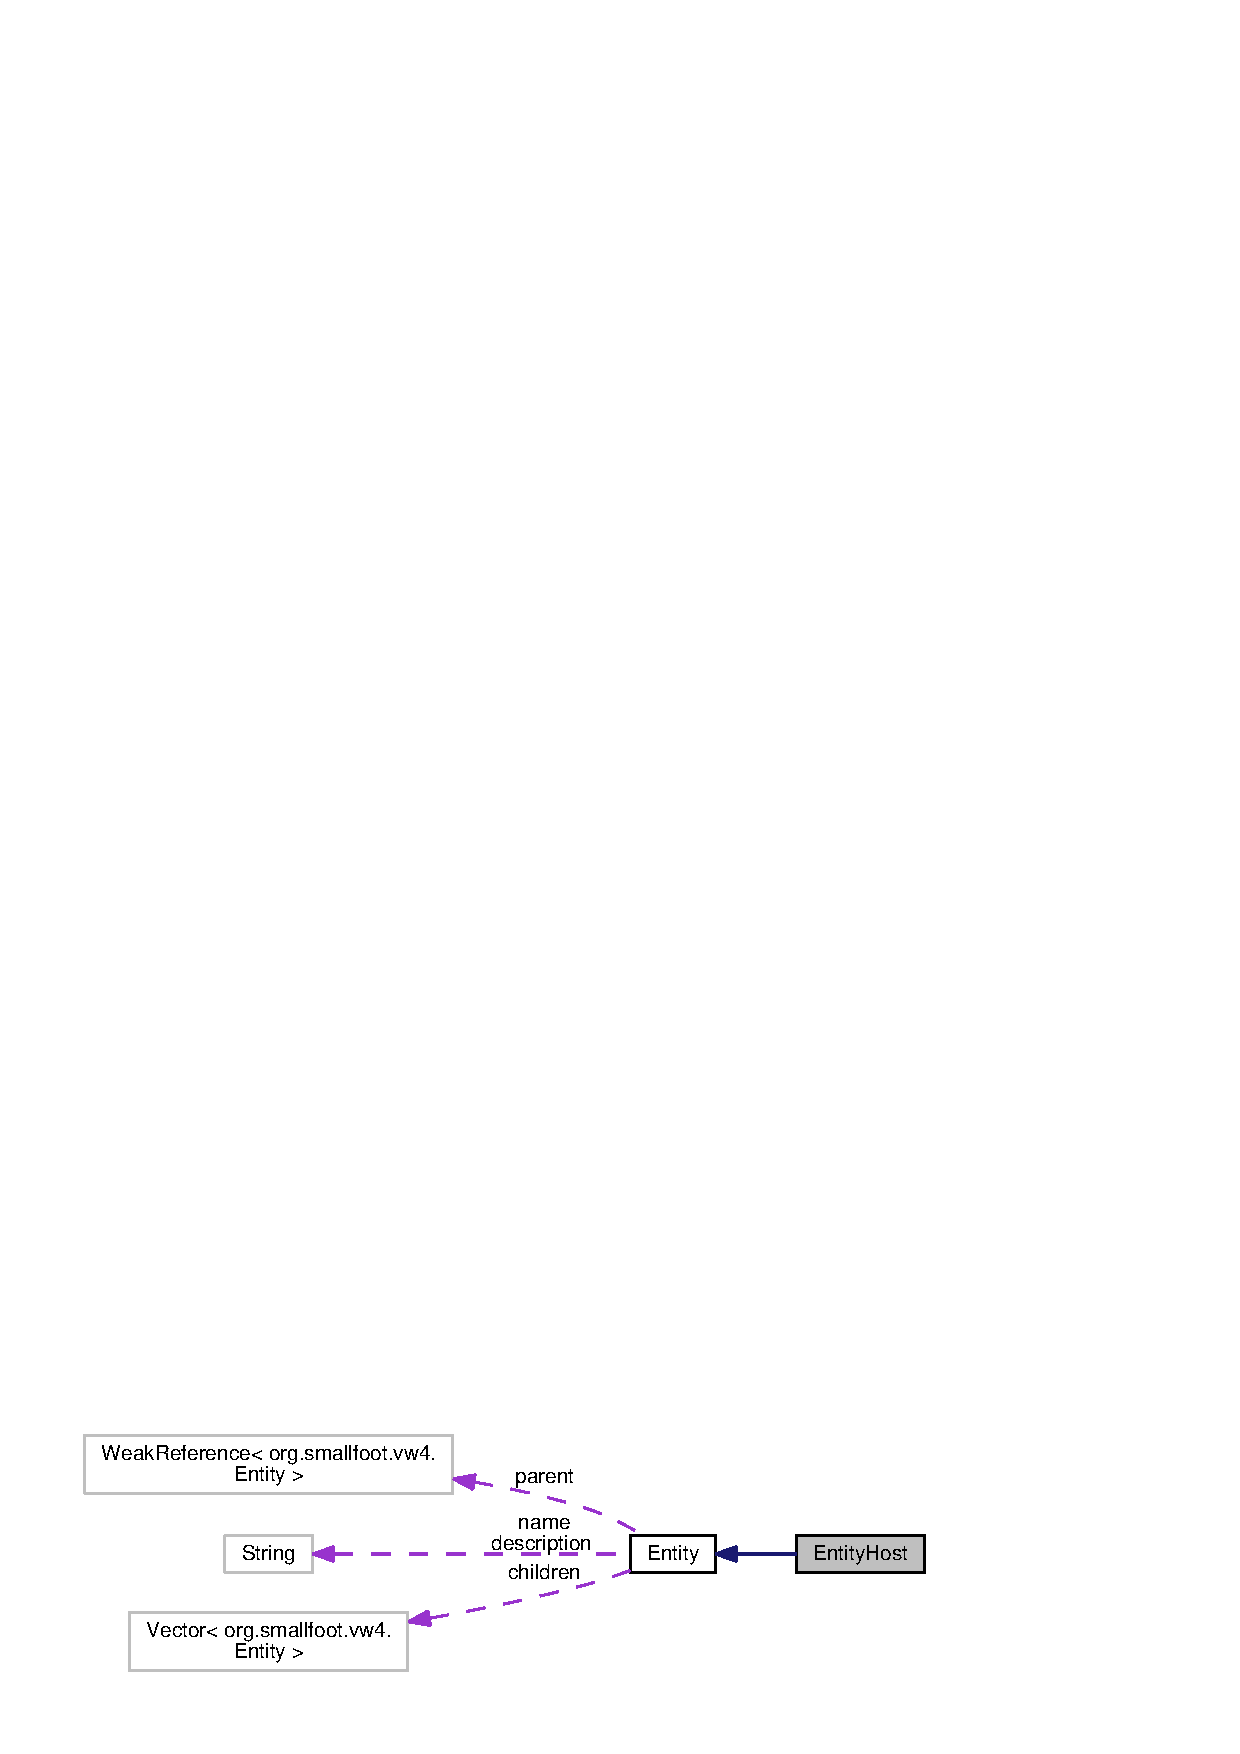
\includegraphics[width=350pt]{classorg_1_1smallfoot_1_1vw4_1_1EntityHost__coll__graph}
\end{center}
\end{figure}
\subsection*{Public Member Functions}
\begin{DoxyCompactItemize}
\item 
{\bf Entity\+Host} (String {\bf name}, {\bf Entity} e)  throws Improper\+Child\+Exception     \label{classorg_1_1smallfoot_1_1vw4_1_1EntityHost_a8c76d8db7cbedb53bd3469b0ec940962}

\begin{DoxyCompactList}\small\item\em Basic Class Constructor. \end{DoxyCompactList}\item 
{\bf Entity} {\bf new\+Parent} (String {\bf name})\label{classorg_1_1smallfoot_1_1vw4_1_1EntityHost_ae3cca685b4cef300a70d257f519a96e4}

\begin{DoxyCompactList}\small\item\em create a new \doxyref{Entity}{p.}{classorg_1_1smallfoot_1_1vw4_1_1Entity} of the correct class to be a parent of this one \end{DoxyCompactList}\end{DoxyCompactItemize}
\subsection*{Protected Member Functions}
\begin{DoxyCompactItemize}
\item 
boolean {\bf can\+Be\+Child} ({\bf Entity} e)
\begin{DoxyCompactList}\small\item\em whether a given entity can be this entity's child \end{DoxyCompactList}\item 
org.\+smallfoot.\+vw4.\+V\+W\+Import.\+Entity {\bf vwentity} (String tag)
\begin{DoxyCompactList}\small\item\em create a streamable J\+S\+O\+N entity from this one \end{DoxyCompactList}\end{DoxyCompactItemize}
\subsection*{Additional Inherited Members}


\subsection{Detailed Description}
An \doxyref{Entity\+Host}{p.}{classorg_1_1smallfoot_1_1vw4_1_1EntityHost} is the representation of an Host entity in the J\+S\+O\+N import for V\+W4. 

Be very careful\+: there is an \doxyref{Entity}{p.}{classorg_1_1smallfoot_1_1vw4_1_1Entity}, and a V\+W\+Import\+::\+Entity 

Definition at line 44 of file Entity\+Host.\+java.



\subsection{Member Function Documentation}
\index{org\+::smallfoot\+::vw4\+::\+Entity\+Host@{org\+::smallfoot\+::vw4\+::\+Entity\+Host}!can\+Be\+Child@{can\+Be\+Child}}
\index{can\+Be\+Child@{can\+Be\+Child}!org\+::smallfoot\+::vw4\+::\+Entity\+Host@{org\+::smallfoot\+::vw4\+::\+Entity\+Host}}
\subsubsection[{can\+Be\+Child}]{\setlength{\rightskip}{0pt plus 5cm}boolean can\+Be\+Child (
\begin{DoxyParamCaption}
\item[{{\bf Entity}}]{e}
\end{DoxyParamCaption}
)\hspace{0.3cm}{\ttfamily [inline]}, {\ttfamily [protected]}}\label{classorg_1_1smallfoot_1_1vw4_1_1EntityHost_a5a51654ce8be38d5f06faa182cb70e61}


whether a given entity can be this entity's child 

\begin{DoxyReturn}{Returns}
true if accepted, false if refused 
\end{DoxyReturn}

\begin{DoxyParams}{Parameters}
{\em e} & entity to check for possible descendent-\/hood \\
\hline
\end{DoxyParams}


Definition at line 55 of file Entity\+Host.\+java.

\index{org\+::smallfoot\+::vw4\+::\+Entity\+Host@{org\+::smallfoot\+::vw4\+::\+Entity\+Host}!vwentity@{vwentity}}
\index{vwentity@{vwentity}!org\+::smallfoot\+::vw4\+::\+Entity\+Host@{org\+::smallfoot\+::vw4\+::\+Entity\+Host}}
\subsubsection[{vwentity}]{\setlength{\rightskip}{0pt plus 5cm}org.\+smallfoot.\+vw4.\+V\+W\+Import.\+Entity vwentity (
\begin{DoxyParamCaption}
\item[{String}]{tag}
\end{DoxyParamCaption}
)\hspace{0.3cm}{\ttfamily [inline]}, {\ttfamily [protected]}}\label{classorg_1_1smallfoot_1_1vw4_1_1EntityHost_a1d6bf85ddf0a9382cfa4f82dd3063473}


create a streamable J\+S\+O\+N entity from this one 

\begin{DoxyReturn}{Returns}
a org.\+smallfoot.\+vw4.\+V\+W\+Import.\+Entity representation of this instance 
\end{DoxyReturn}

\begin{DoxyParams}{Parameters}
{\em tag} & default tag to apply \\
\hline
\end{DoxyParams}


Definition at line 61 of file Entity\+Host.\+java.



References Entity.\+children(), Entity.\+description(), and Entity.\+name().



Here is the call graph for this function\+:\nopagebreak
\begin{figure}[H]
\begin{center}
\leavevmode
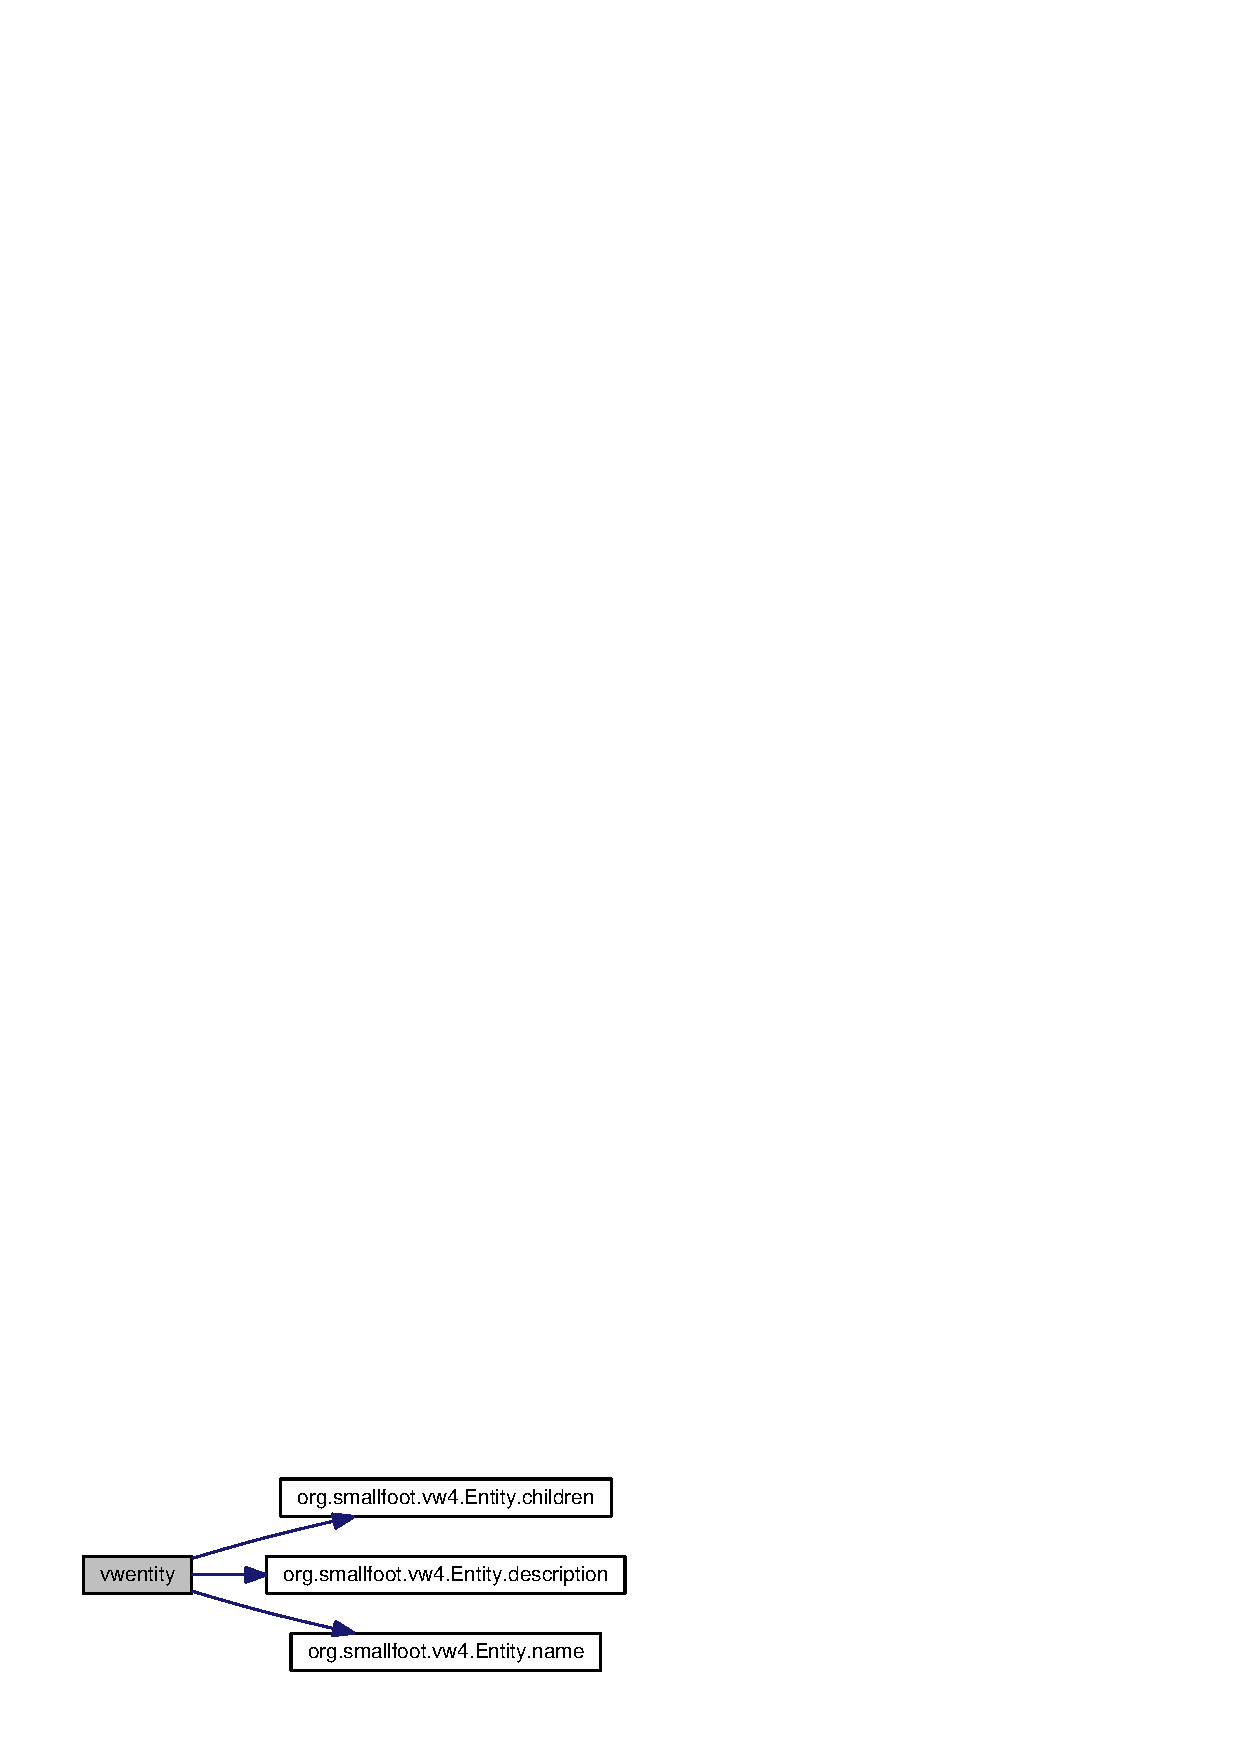
\includegraphics[width=304pt]{classorg_1_1smallfoot_1_1vw4_1_1EntityHost_a1d6bf85ddf0a9382cfa4f82dd3063473_cgraph}
\end{center}
\end{figure}




The documentation for this class was generated from the following file\+:\begin{DoxyCompactItemize}
\item 
java/{\bf Entity\+Host.\+java}\end{DoxyCompactItemize}

\section{Virtual\+Wisdom4\+Client\+Tool.\+Entity\+Selector Interface Reference}
\label{interfaceorg_1_1smallfoot_1_1vw4_1_1VirtualWisdom4ClientTool_1_1EntitySelector}\index{Virtual\+Wisdom4\+Client\+Tool.\+Entity\+Selector@{Virtual\+Wisdom4\+Client\+Tool.\+Entity\+Selector}}


simple convenience interface to allow entity selection to be codified and created on-\/the-\/fly in a query A\+P\+I  


\subsection*{Public Member Functions}
\begin{DoxyCompactItemize}
\item 
boolean {\bf select} ({\bf Entity} e)
\begin{DoxyCompactList}\small\item\em function to define whether an entity should be selected based on its attributes \end{DoxyCompactList}\end{DoxyCompactItemize}


\subsection{Detailed Description}
simple convenience interface to allow entity selection to be codified and created on-\/the-\/fly in a query A\+P\+I 

Definition at line 603 of file Virtual\+Wisdom4\+Client\+Tool.\+java.



\subsection{Member Function Documentation}
\index{org\+::smallfoot\+::vw4\+::\+Virtual\+Wisdom4\+Client\+Tool\+::\+Entity\+Selector@{org\+::smallfoot\+::vw4\+::\+Virtual\+Wisdom4\+Client\+Tool\+::\+Entity\+Selector}!select@{select}}
\index{select@{select}!org\+::smallfoot\+::vw4\+::\+Virtual\+Wisdom4\+Client\+Tool\+::\+Entity\+Selector@{org\+::smallfoot\+::vw4\+::\+Virtual\+Wisdom4\+Client\+Tool\+::\+Entity\+Selector}}
\subsubsection[{select}]{\setlength{\rightskip}{0pt plus 5cm}boolean select (
\begin{DoxyParamCaption}
\item[{{\bf Entity}}]{e}
\end{DoxyParamCaption}
)}\label{interfaceorg_1_1smallfoot_1_1vw4_1_1VirtualWisdom4ClientTool_1_1EntitySelector_a06dae9b60fcb30b8dc2ce7d716a56548}


function to define whether an entity should be selected based on its attributes 


\begin{DoxyParams}{Parameters}
{\em e} & entity to consider \\
\hline
\end{DoxyParams}
\begin{DoxyReturn}{Returns}
true if this entity satisfies the coded logic 
\end{DoxyReturn}


The documentation for this interface was generated from the following file\+:\begin{DoxyCompactItemize}
\item 
java/{\bf Virtual\+Wisdom4\+Client\+Tool.\+java}\end{DoxyCompactItemize}

\section{Entity.\+Improper\+Child\+Exception Class Reference}
\label{classorg_1_1smallfoot_1_1vw4_1_1Entity_1_1ImproperChildException}\index{Entity.\+Improper\+Child\+Exception@{Entity.\+Improper\+Child\+Exception}}


Descendents of \doxyref{Entity}{p.}{classorg_1_1smallfoot_1_1vw4_1_1Entity} should know whether a given entity can be one of their child elements.  




Inheritance diagram for Entity.\+Improper\+Child\+Exception\+:\nopagebreak
\begin{figure}[H]
\begin{center}
\leavevmode
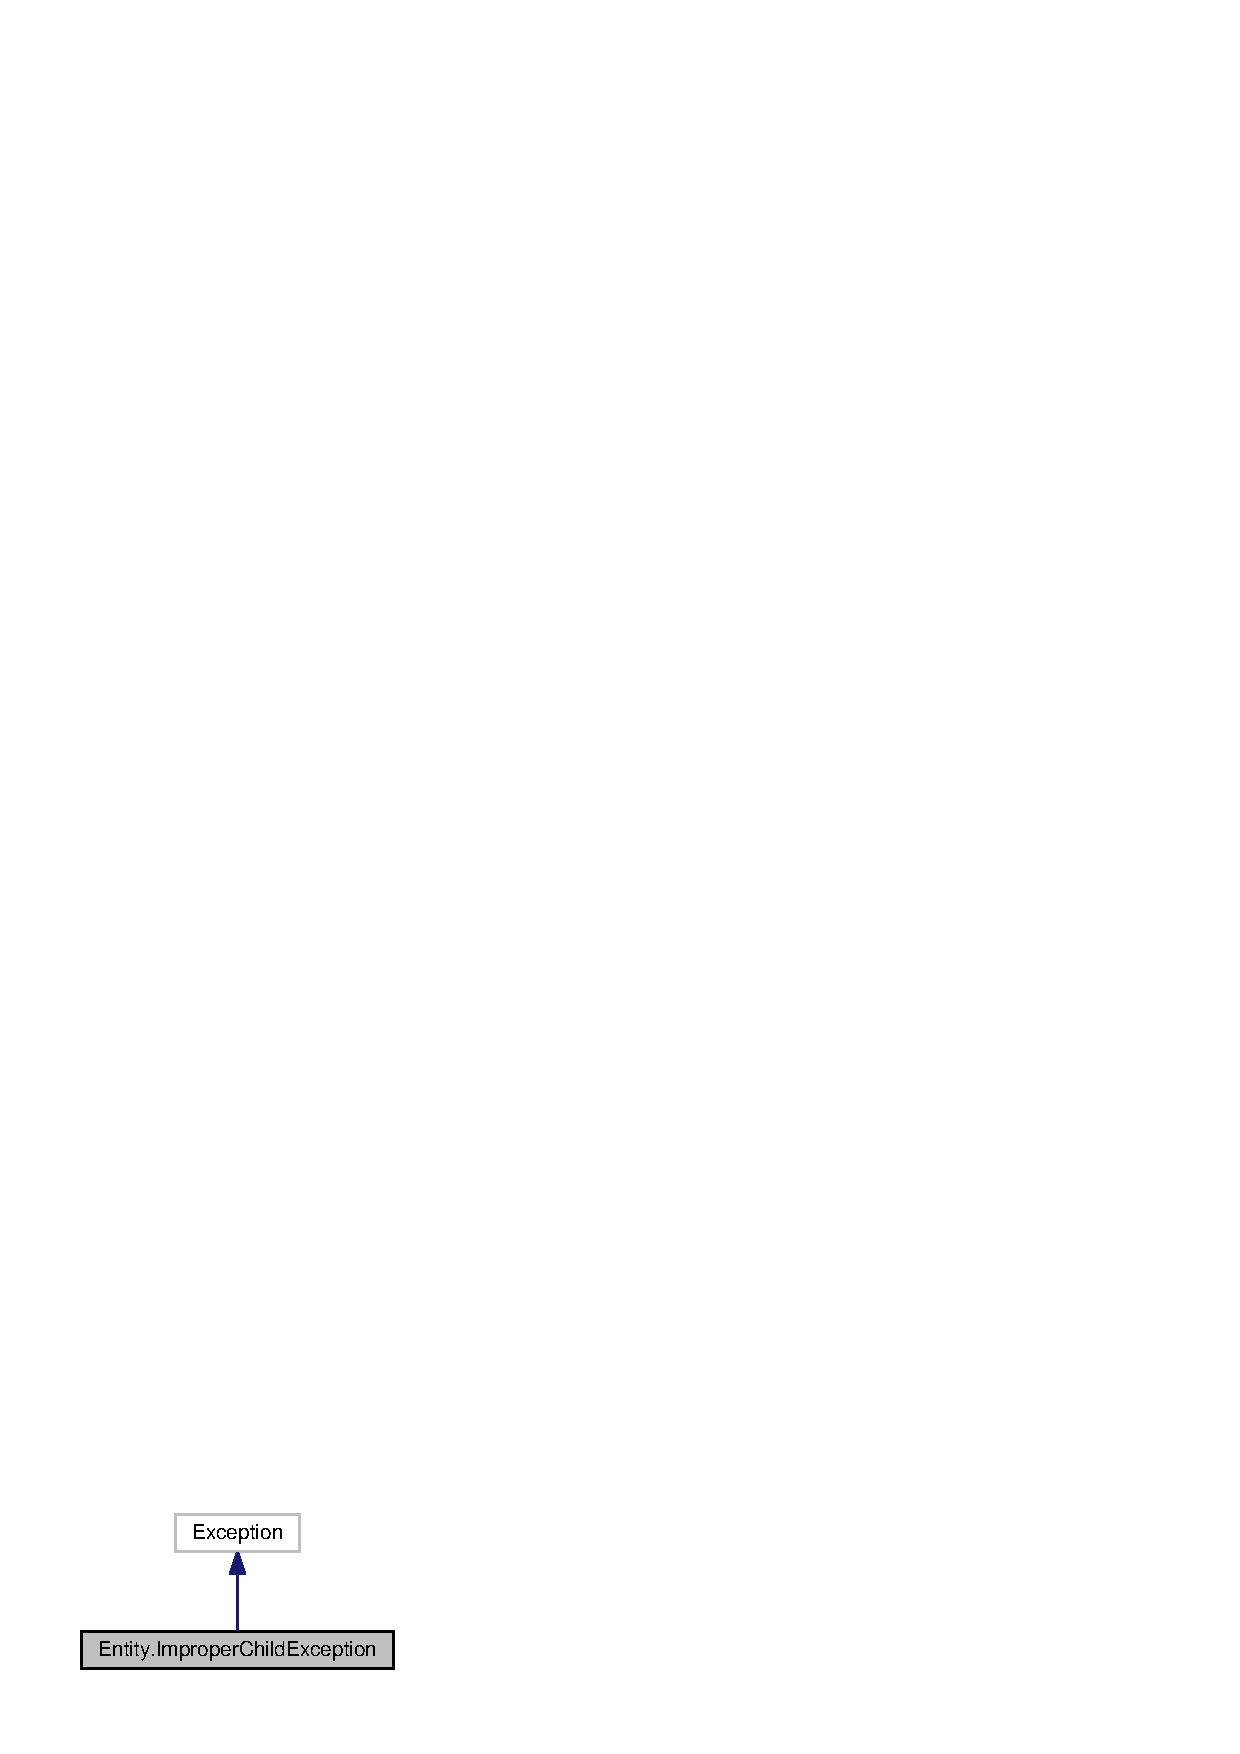
\includegraphics[width=192pt]{classorg_1_1smallfoot_1_1vw4_1_1Entity_1_1ImproperChildException__inherit__graph}
\end{center}
\end{figure}


Collaboration diagram for Entity.\+Improper\+Child\+Exception\+:\nopagebreak
\begin{figure}[H]
\begin{center}
\leavevmode
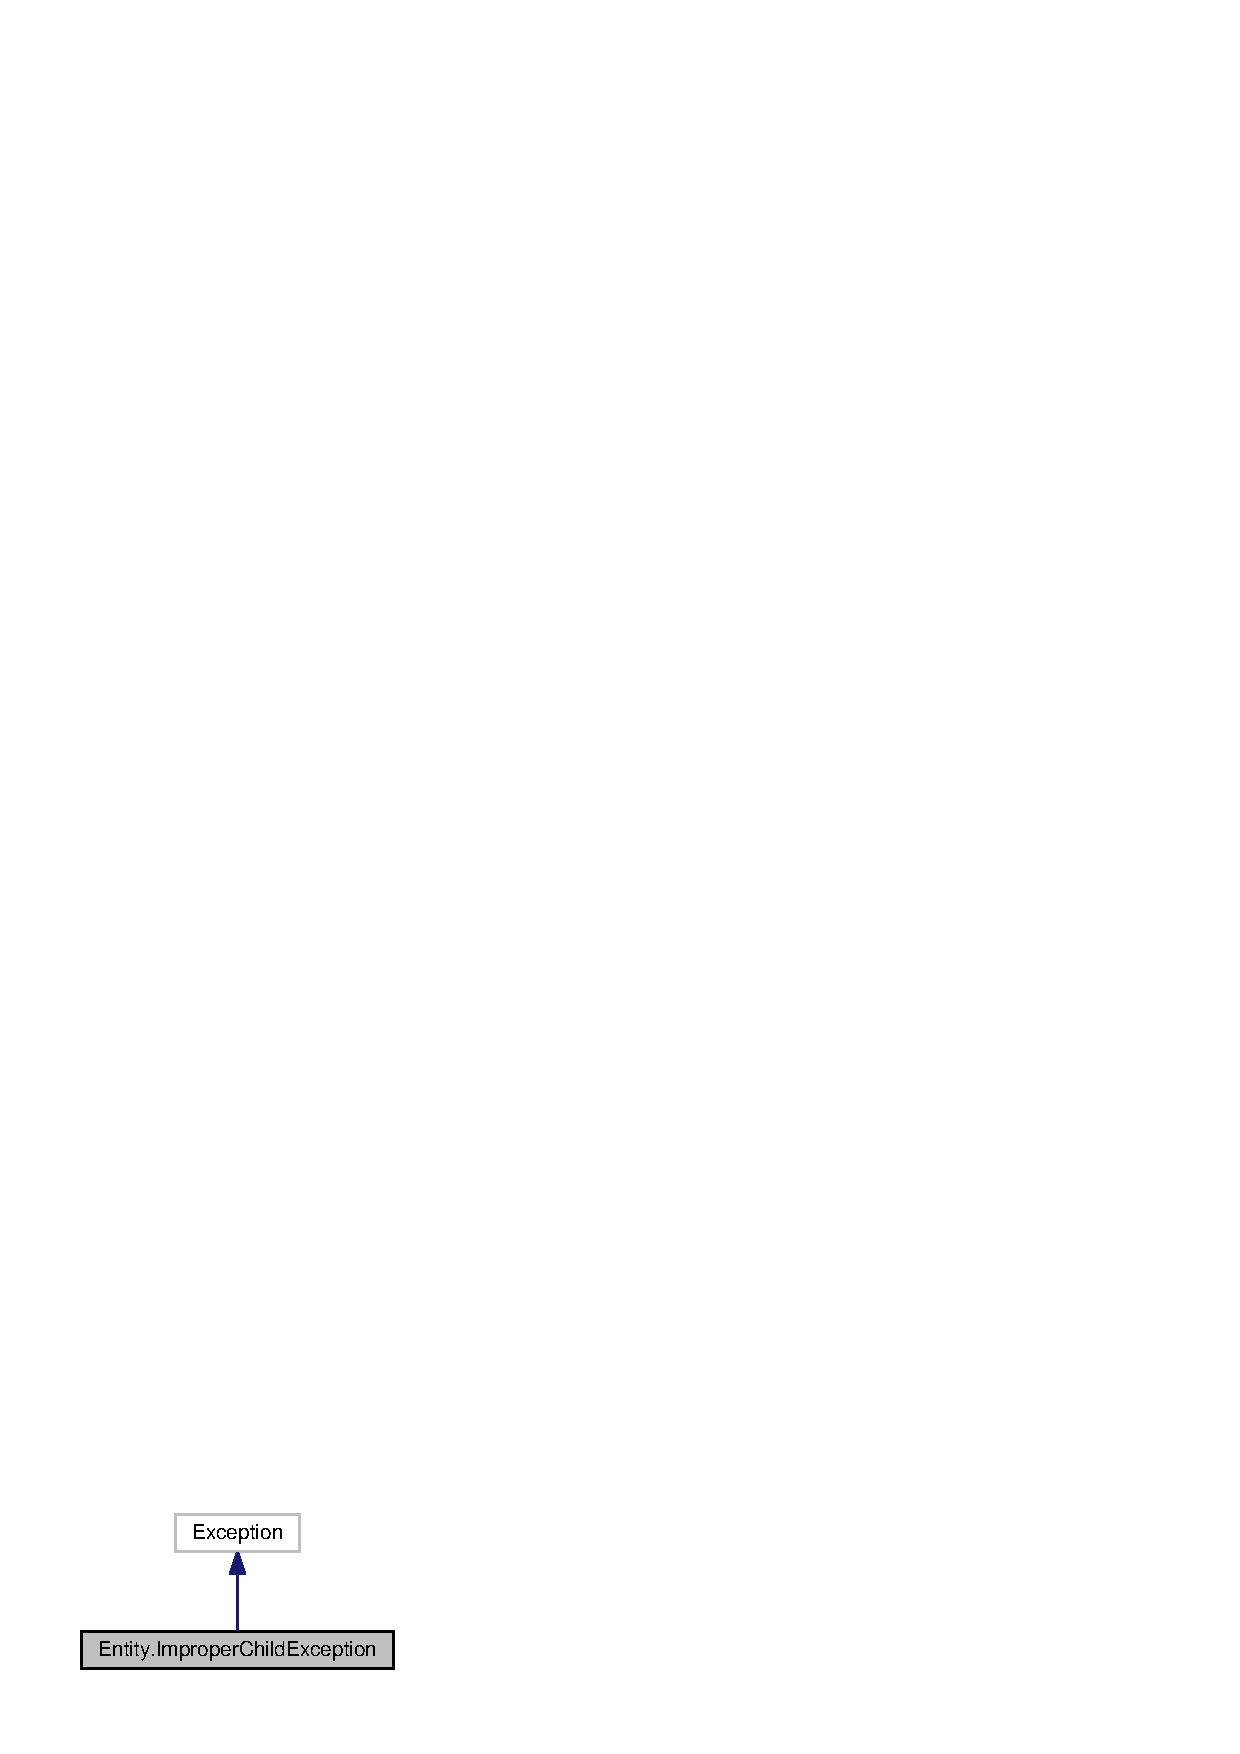
\includegraphics[width=192pt]{classorg_1_1smallfoot_1_1vw4_1_1Entity_1_1ImproperChildException__coll__graph}
\end{center}
\end{figure}
\subsection*{Public Member Functions}
\begin{DoxyCompactItemize}
\item 
{\bf Improper\+Child\+Exception} (String s)
\begin{DoxyCompactList}\small\item\em create a new instance with the given message \end{DoxyCompactList}\item 
{\bf Improper\+Child\+Exception} ({\bf Entity} e, {\bf Entity} p)
\begin{DoxyCompactList}\small\item\em create a new instance with a consistent message based on the entities offered \end{DoxyCompactList}\end{DoxyCompactItemize}


\subsection{Detailed Description}
Descendents of \doxyref{Entity}{p.}{classorg_1_1smallfoot_1_1vw4_1_1Entity} should know whether a given entity can be one of their child elements. 

This exception is intended as a method of signalling -- and rippling up if necessary -- than an intended seconding as a child element is not accepted by the would-\/be parent. 

Definition at line 123 of file Entity.\+java.



\subsection{Constructor \& Destructor Documentation}
\index{org\+::smallfoot\+::vw4\+::\+Entity\+::\+Improper\+Child\+Exception@{org\+::smallfoot\+::vw4\+::\+Entity\+::\+Improper\+Child\+Exception}!Improper\+Child\+Exception@{Improper\+Child\+Exception}}
\index{Improper\+Child\+Exception@{Improper\+Child\+Exception}!org\+::smallfoot\+::vw4\+::\+Entity\+::\+Improper\+Child\+Exception@{org\+::smallfoot\+::vw4\+::\+Entity\+::\+Improper\+Child\+Exception}}
\subsubsection[{Improper\+Child\+Exception}]{\setlength{\rightskip}{0pt plus 5cm}{\bf Improper\+Child\+Exception} (
\begin{DoxyParamCaption}
\item[{String}]{s}
\end{DoxyParamCaption}
)\hspace{0.3cm}{\ttfamily [inline]}}\label{classorg_1_1smallfoot_1_1vw4_1_1Entity_1_1ImproperChildException_a5c306b76ca66e2e9744e4e1f637cc991}


create a new instance with the given message 


\begin{DoxyParams}{Parameters}
{\em s} & description to encapsulate \\
\hline
\end{DoxyParams}


Definition at line 126 of file Entity.\+java.

\index{org\+::smallfoot\+::vw4\+::\+Entity\+::\+Improper\+Child\+Exception@{org\+::smallfoot\+::vw4\+::\+Entity\+::\+Improper\+Child\+Exception}!Improper\+Child\+Exception@{Improper\+Child\+Exception}}
\index{Improper\+Child\+Exception@{Improper\+Child\+Exception}!org\+::smallfoot\+::vw4\+::\+Entity\+::\+Improper\+Child\+Exception@{org\+::smallfoot\+::vw4\+::\+Entity\+::\+Improper\+Child\+Exception}}
\subsubsection[{Improper\+Child\+Exception}]{\setlength{\rightskip}{0pt plus 5cm}{\bf Improper\+Child\+Exception} (
\begin{DoxyParamCaption}
\item[{{\bf Entity}}]{e, }
\item[{{\bf Entity}}]{p}
\end{DoxyParamCaption}
)\hspace{0.3cm}{\ttfamily [inline]}}\label{classorg_1_1smallfoot_1_1vw4_1_1Entity_1_1ImproperChildException_a2a8c52dc01b9775f76eab69ebc825638}


create a new instance with a consistent message based on the entities offered 


\begin{DoxyParams}{Parameters}
{\em e} & child entity \\
\hline
{\em p} & parent entity \\
\hline
\end{DoxyParams}


Definition at line 132 of file Entity.\+java.



The documentation for this class was generated from the following file\+:\begin{DoxyCompactItemize}
\item 
java/{\bf Entity.\+java}\end{DoxyCompactItemize}

\section{Entity.\+Leaf\+Entity Class Reference}
\label{classorg_1_1smallfoot_1_1vw4_1_1Entity_1_1LeafEntity}\index{Entity.\+Leaf\+Entity@{Entity.\+Leaf\+Entity}}


A \doxyref{Leaf\+Entity}{p.}{classorg_1_1smallfoot_1_1vw4_1_1Entity_1_1LeafEntity} is the common ancestor of Storage F\+As and Server H\+B\+As; this is combined only so that leaves can be treated in common.  




Inheritance diagram for Entity.\+Leaf\+Entity\+:\nopagebreak
\begin{figure}[H]
\begin{center}
\leavevmode
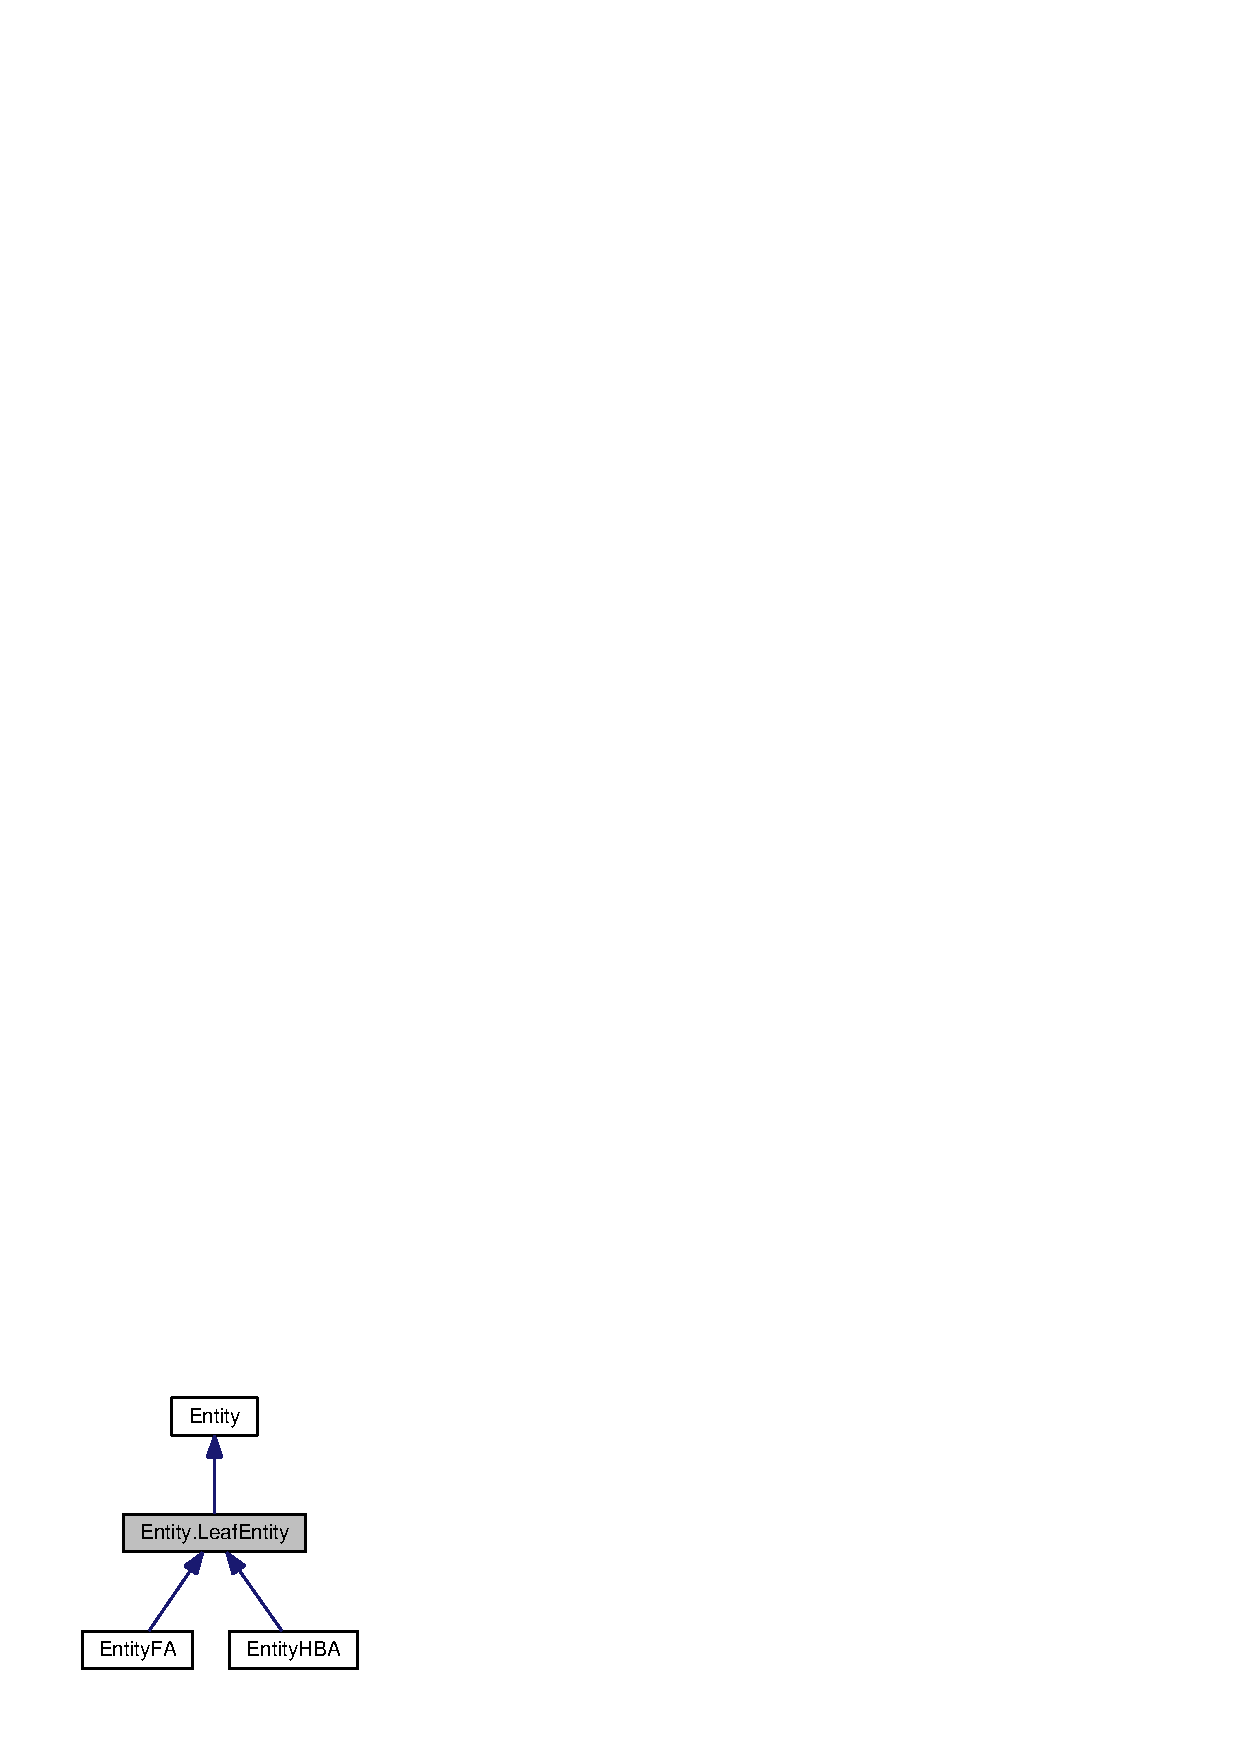
\includegraphics[width=175pt]{classorg_1_1smallfoot_1_1vw4_1_1Entity_1_1LeafEntity__inherit__graph}
\end{center}
\end{figure}


Collaboration diagram for Entity.\+Leaf\+Entity\+:\nopagebreak
\begin{figure}[H]
\begin{center}
\leavevmode
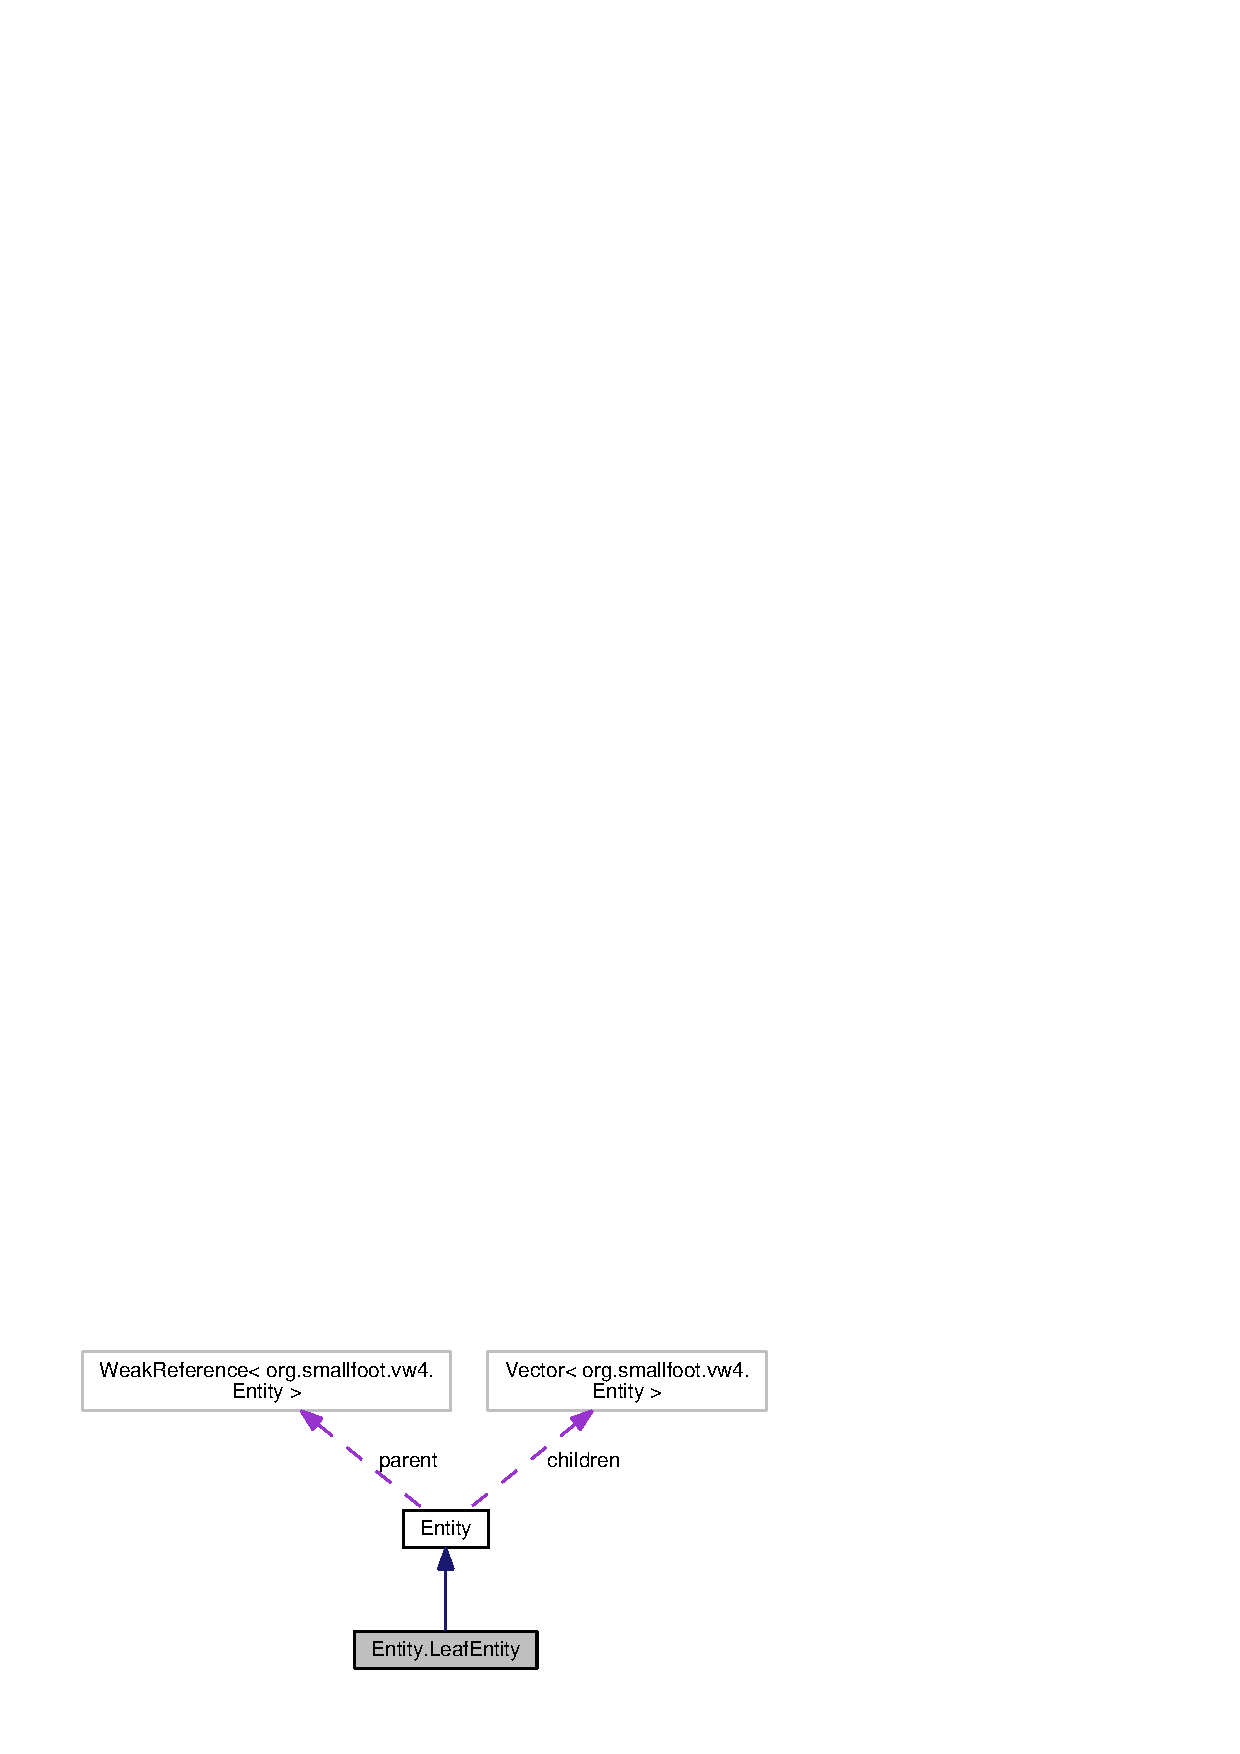
\includegraphics[width=350pt]{classorg_1_1smallfoot_1_1vw4_1_1Entity_1_1LeafEntity__coll__graph}
\end{center}
\end{figure}
\subsection*{Public Member Functions}
\begin{DoxyCompactItemize}
\item 
{\bf Leaf\+Entity} (String {\bf name}, String {\bf wwn})
\begin{DoxyCompactList}\small\item\em Class Constructor with an initial child to absorb. \end{DoxyCompactList}\item 
{\bf Entity} {\bf new\+Parent} (String {\bf name})
\begin{DoxyCompactList}\small\item\em create a new \doxyref{Entity}{p.}{classorg_1_1smallfoot_1_1vw4_1_1Entity} of the correct class to be a parent of this one\+: this function is stubbed to return null so that this class can be a static class and directly extensible. \end{DoxyCompactList}\item 
String {\bf parent\+Name} ()
\begin{DoxyCompactList}\small\item\em convenience function\+: if this entity has a parent, show the parent's name, otherwise show this entity's name. \end{DoxyCompactList}\item 
String {\bf wwn} ()
\begin{DoxyCompactList}\small\item\em the unique W\+W\+P\+N of the hba\+: getter for internal variable \end{DoxyCompactList}\end{DoxyCompactItemize}
\subsection*{Protected Member Functions}
\begin{DoxyCompactItemize}
\item 
boolean {\bf can\+Be\+Child} ({\bf Entity} e)
\begin{DoxyCompactList}\small\item\em whether a given entity can be this entity's child \end{DoxyCompactList}\item 
org.\+smallfoot.\+vw4.\+V\+W\+Import.\+Entity {\bf vwentity} (String tag)\label{classorg_1_1smallfoot_1_1vw4_1_1Entity_1_1LeafEntity_a1d6bf85ddf0a9382cfa4f82dd3063473}

\begin{DoxyCompactList}\small\item\em create a bogus function to avoid build errors \end{DoxyCompactList}\end{DoxyCompactItemize}
\subsection*{Protected Attributes}
\begin{DoxyCompactItemize}
\item 
String {\bf wwn}\label{classorg_1_1smallfoot_1_1vw4_1_1Entity_1_1LeafEntity_ab07f595ad2e4da7c53cd29f435f5bb3c}

\begin{DoxyCompactList}\small\item\em the unique W\+W\+P\+N of the hba \end{DoxyCompactList}\end{DoxyCompactItemize}


\subsection{Detailed Description}
A \doxyref{Leaf\+Entity}{p.}{classorg_1_1smallfoot_1_1vw4_1_1Entity_1_1LeafEntity} is the common ancestor of Storage F\+As and Server H\+B\+As; this is combined only so that leaves can be treated in common. 

Definition at line 202 of file Entity.\+java.



\subsection{Constructor \& Destructor Documentation}
\index{org\+::smallfoot\+::vw4\+::\+Entity\+::\+Leaf\+Entity@{org\+::smallfoot\+::vw4\+::\+Entity\+::\+Leaf\+Entity}!Leaf\+Entity@{Leaf\+Entity}}
\index{Leaf\+Entity@{Leaf\+Entity}!org\+::smallfoot\+::vw4\+::\+Entity\+::\+Leaf\+Entity@{org\+::smallfoot\+::vw4\+::\+Entity\+::\+Leaf\+Entity}}
\subsubsection[{Leaf\+Entity}]{\setlength{\rightskip}{0pt plus 5cm}{\bf Leaf\+Entity} (
\begin{DoxyParamCaption}
\item[{String}]{name, }
\item[{String}]{wwn}
\end{DoxyParamCaption}
)\hspace{0.3cm}{\ttfamily [inline]}}\label{classorg_1_1smallfoot_1_1vw4_1_1Entity_1_1LeafEntity_a30cc6402437a41c9da17a4e50fc9590c}


Class Constructor with an initial child to absorb. 


\begin{DoxyParams}{Parameters}
{\em name} & initial name of the new entity \\
\hline
{\em wwn} & initial child entity for this Leaf \doxyref{Entity}{p.}{classorg_1_1smallfoot_1_1vw4_1_1Entity} \\
\hline
\end{DoxyParams}


Definition at line 233 of file Entity.\+java.



References Entity.\+Leaf\+Entity.\+wwn().



Here is the call graph for this function\+:\nopagebreak
\begin{figure}[H]
\begin{center}
\leavevmode
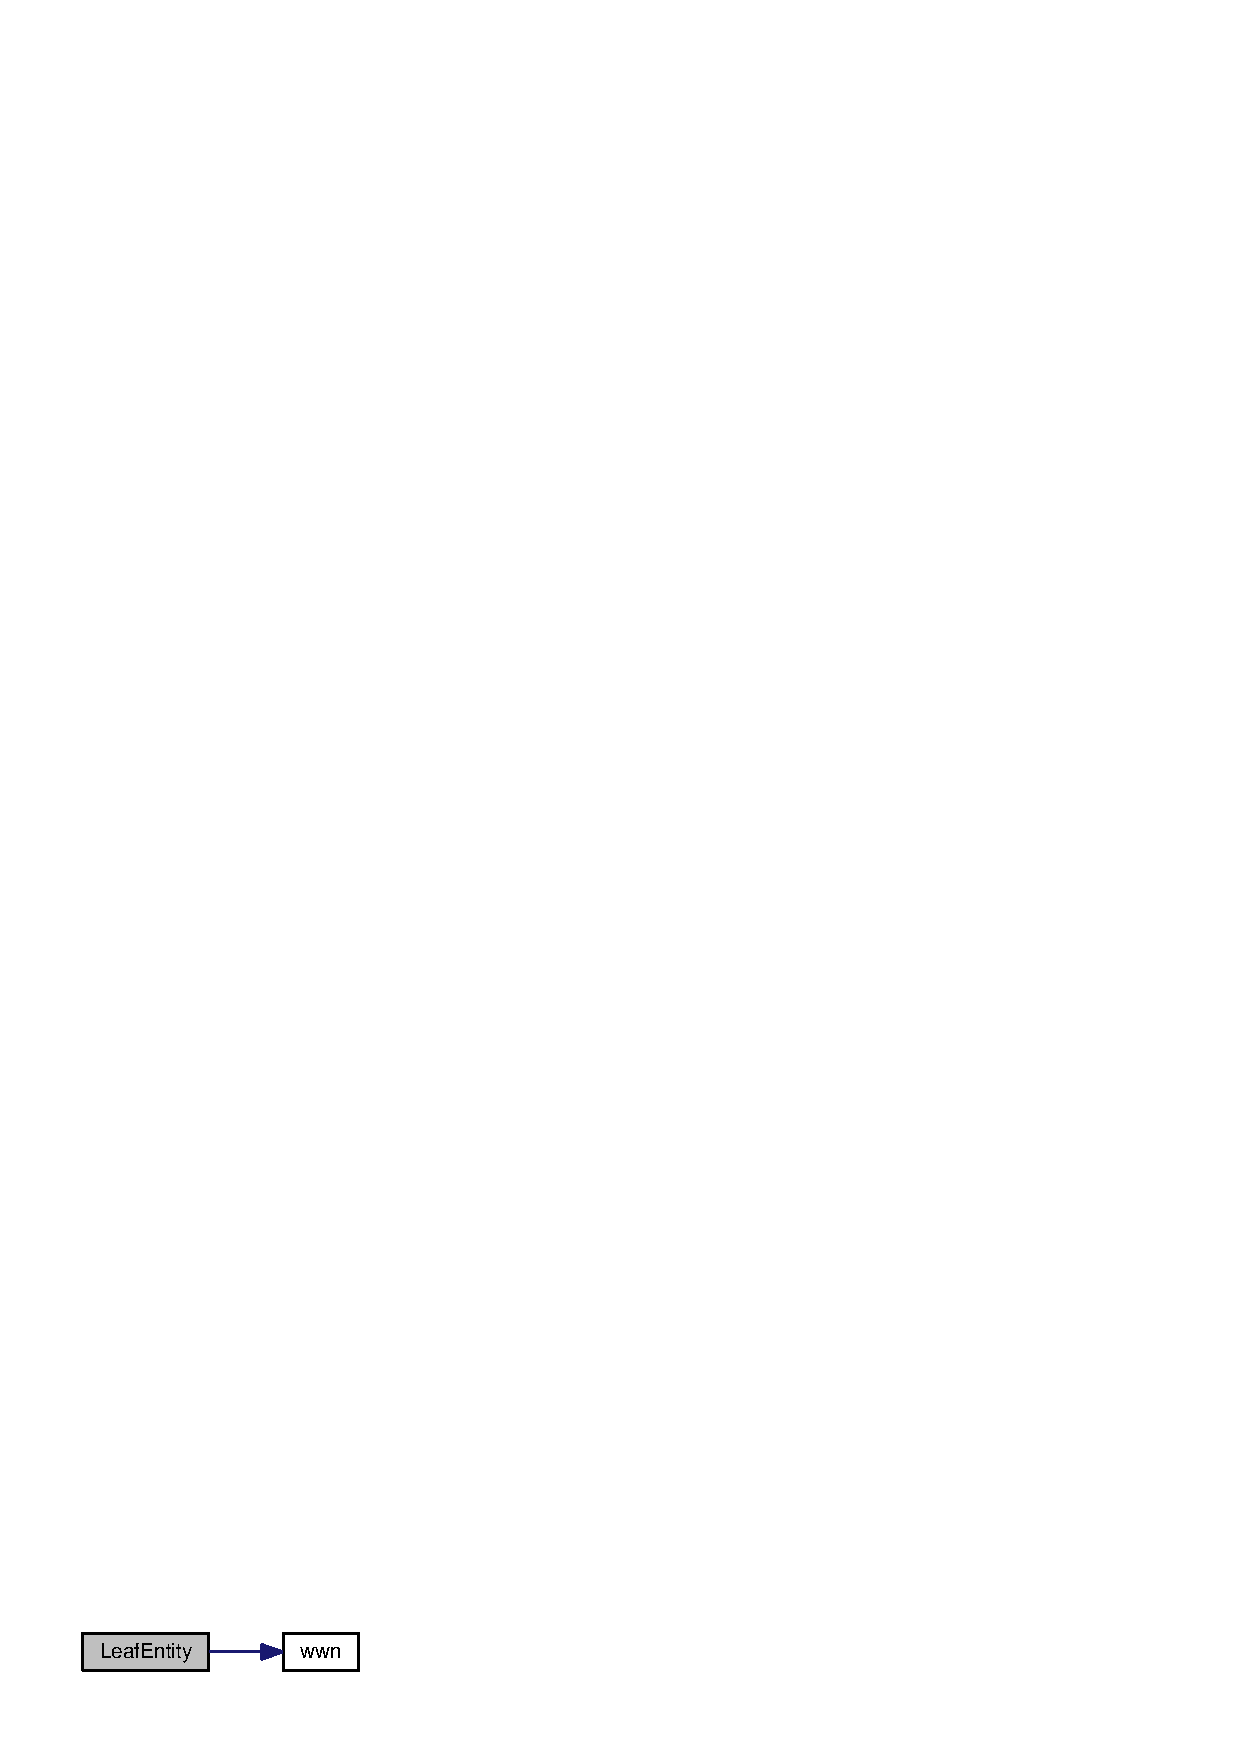
\includegraphics[width=176pt]{classorg_1_1smallfoot_1_1vw4_1_1Entity_1_1LeafEntity_a30cc6402437a41c9da17a4e50fc9590c_cgraph}
\end{center}
\end{figure}




\subsection{Member Function Documentation}
\index{org\+::smallfoot\+::vw4\+::\+Entity\+::\+Leaf\+Entity@{org\+::smallfoot\+::vw4\+::\+Entity\+::\+Leaf\+Entity}!can\+Be\+Child@{can\+Be\+Child}}
\index{can\+Be\+Child@{can\+Be\+Child}!org\+::smallfoot\+::vw4\+::\+Entity\+::\+Leaf\+Entity@{org\+::smallfoot\+::vw4\+::\+Entity\+::\+Leaf\+Entity}}
\subsubsection[{can\+Be\+Child}]{\setlength{\rightskip}{0pt plus 5cm}boolean can\+Be\+Child (
\begin{DoxyParamCaption}
\item[{{\bf Entity}}]{e}
\end{DoxyParamCaption}
)\hspace{0.3cm}{\ttfamily [inline]}, {\ttfamily [protected]}}\label{classorg_1_1smallfoot_1_1vw4_1_1Entity_1_1LeafEntity_a5a51654ce8be38d5f06faa182cb70e61}


whether a given entity can be this entity's child 

\begin{DoxyReturn}{Returns}
true if accepted, false if refused. \doxyref{Leaf\+Entity}{p.}{classorg_1_1smallfoot_1_1vw4_1_1Entity_1_1LeafEntity} has no children so this method will always be false
\end{DoxyReturn}

\begin{DoxyParams}{Parameters}
{\em e} & entity to check for possible descendent-\/hood \\
\hline
\end{DoxyParams}
\begin{DoxyReturn}{Returns}
true if this entity accepts children of \char`\"{}e\char`\"{}'s descendent type (always false for Leaf \doxyref{Entity}{p.}{classorg_1_1smallfoot_1_1vw4_1_1Entity}) 
\end{DoxyReturn}


Definition at line 246 of file Entity.\+java.

\index{org\+::smallfoot\+::vw4\+::\+Entity\+::\+Leaf\+Entity@{org\+::smallfoot\+::vw4\+::\+Entity\+::\+Leaf\+Entity}!new\+Parent@{new\+Parent}}
\index{new\+Parent@{new\+Parent}!org\+::smallfoot\+::vw4\+::\+Entity\+::\+Leaf\+Entity@{org\+::smallfoot\+::vw4\+::\+Entity\+::\+Leaf\+Entity}}
\subsubsection[{new\+Parent}]{\setlength{\rightskip}{0pt plus 5cm}{\bf Entity} new\+Parent (
\begin{DoxyParamCaption}
\item[{String}]{name}
\end{DoxyParamCaption}
)\hspace{0.3cm}{\ttfamily [inline]}}\label{classorg_1_1smallfoot_1_1vw4_1_1Entity_1_1LeafEntity_ae3cca685b4cef300a70d257f519a96e4}


create a new \doxyref{Entity}{p.}{classorg_1_1smallfoot_1_1vw4_1_1Entity} of the correct class to be a parent of this one\+: this function is stubbed to return null so that this class can be a static class and directly extensible. 

Not really 100\% good practice, but the descendency of this \doxyref{Leaf\+Entity}{p.}{classorg_1_1smallfoot_1_1vw4_1_1Entity_1_1LeafEntity} is intended to collect functionality. This class is wrapped inside an \doxyref{Entity}{p.}{classorg_1_1smallfoot_1_1vw4_1_1Entity} to retain a clear affinity, but thence needs to be static to be extensible. \char`\"{}\+She swallowed the cat to catch the spider, she swallowed the
spider to catch the fly.. \char`\"{}

Descendents will override this method

\begin{DoxyReturn}{Returns}
new parent for this entity 
\end{DoxyReturn}

\begin{DoxyParams}{Parameters}
{\em name} & initial name of the new entity \\
\hline
\end{DoxyParams}


Definition at line 271 of file Entity.\+java.

\index{org\+::smallfoot\+::vw4\+::\+Entity\+::\+Leaf\+Entity@{org\+::smallfoot\+::vw4\+::\+Entity\+::\+Leaf\+Entity}!parent\+Name@{parent\+Name}}
\index{parent\+Name@{parent\+Name}!org\+::smallfoot\+::vw4\+::\+Entity\+::\+Leaf\+Entity@{org\+::smallfoot\+::vw4\+::\+Entity\+::\+Leaf\+Entity}}
\subsubsection[{parent\+Name}]{\setlength{\rightskip}{0pt plus 5cm}String parent\+Name (
\begin{DoxyParamCaption}
{}
\end{DoxyParamCaption}
)\hspace{0.3cm}{\ttfamily [inline]}}\label{classorg_1_1smallfoot_1_1vw4_1_1Entity_1_1LeafEntity_a929a7f5f05728b26869df0351a7a815d}


convenience function\+: if this entity has a parent, show the parent's name, otherwise show this entity's name. 

Used during Ordered\+Tuples written via Virtual\+Wisdom4\+Client\+Tool.\+write\+Ordered\+Tuples(\+String, Entity\+Selector), this allows a simpler, consistent coding when Ordered\+Tuples is being exported.

\begin{DoxyReturn}{Returns}
name of parent entity is existent, otherwise name of this entity 
\end{DoxyReturn}


Definition at line 219 of file Entity.\+java.



References Entity.\+name().



Here is the call graph for this function\+:\nopagebreak
\begin{figure}[H]
\begin{center}
\leavevmode
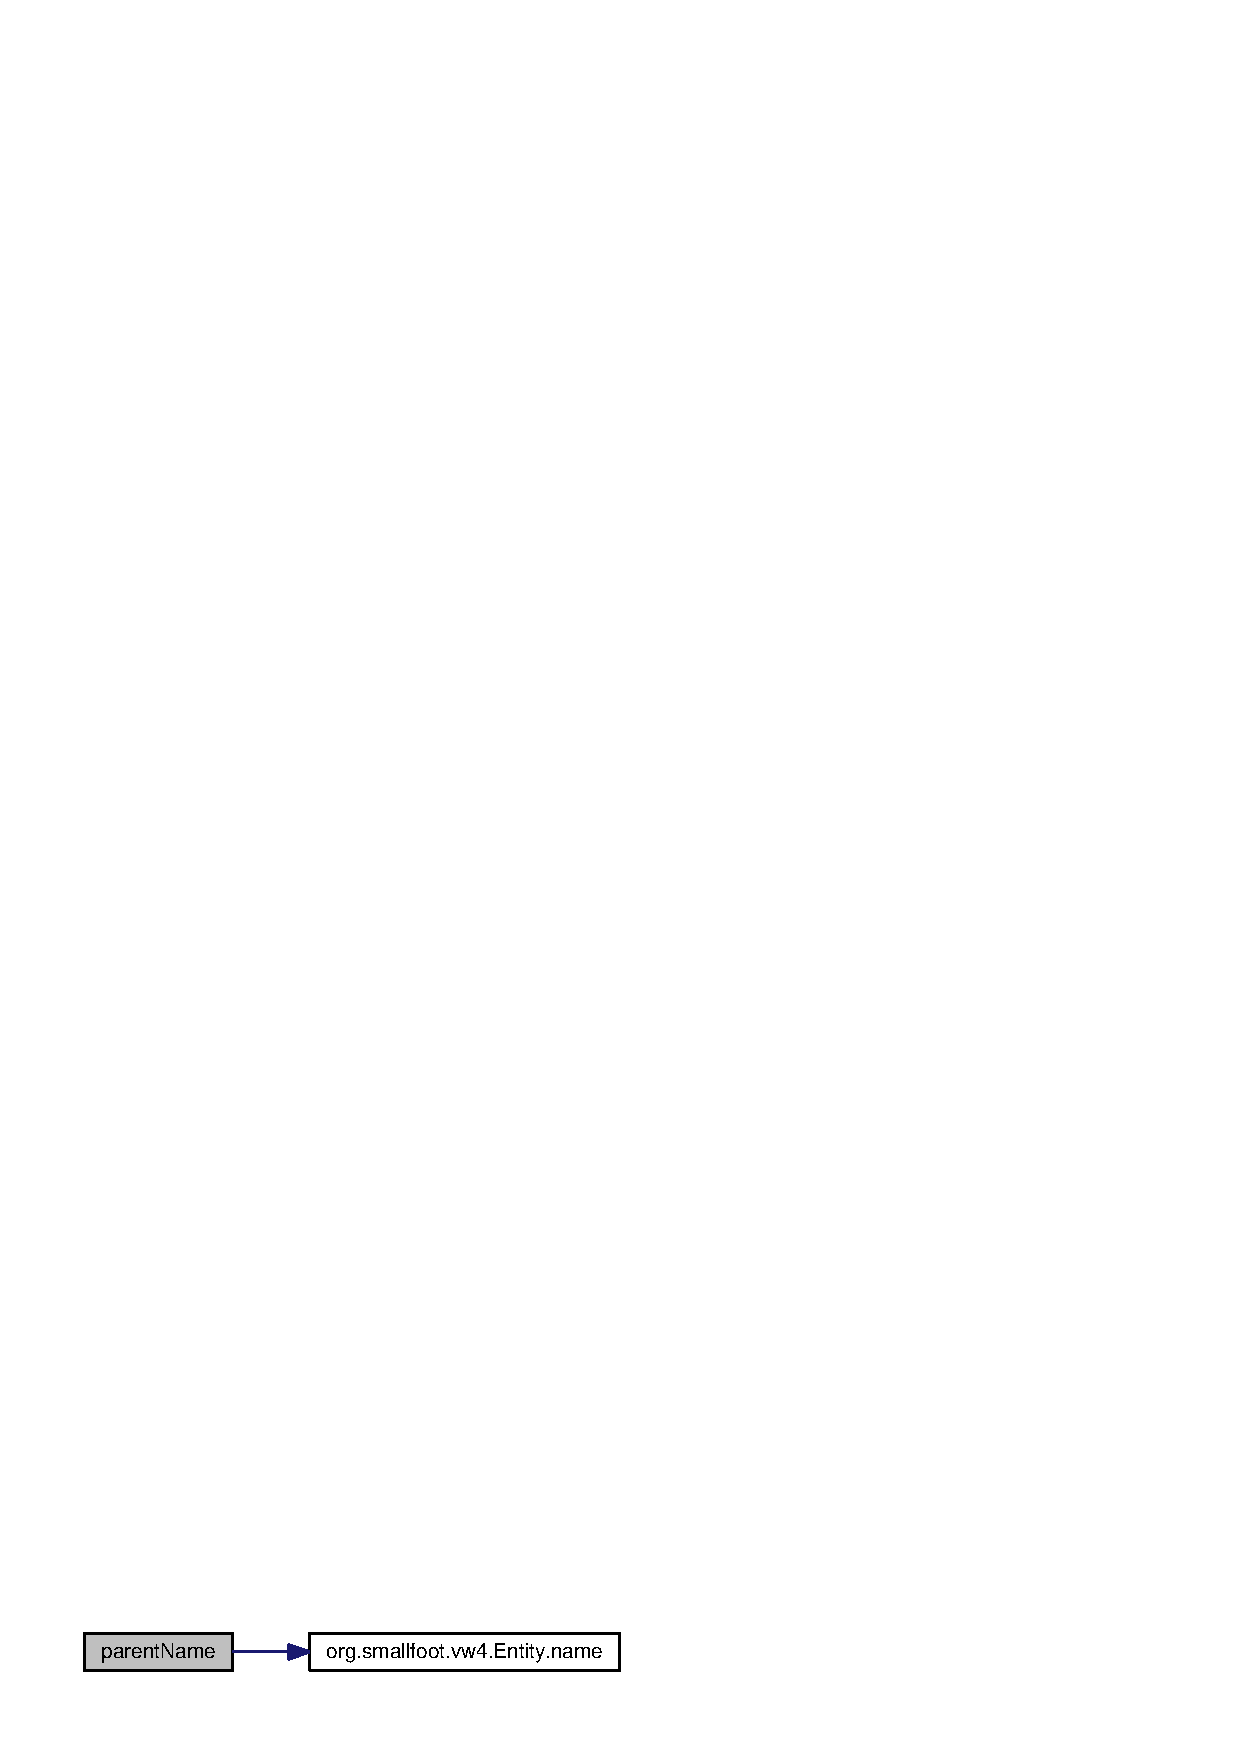
\includegraphics[width=302pt]{classorg_1_1smallfoot_1_1vw4_1_1Entity_1_1LeafEntity_a929a7f5f05728b26869df0351a7a815d_cgraph}
\end{center}
\end{figure}


\index{org\+::smallfoot\+::vw4\+::\+Entity\+::\+Leaf\+Entity@{org\+::smallfoot\+::vw4\+::\+Entity\+::\+Leaf\+Entity}!wwn@{wwn}}
\index{wwn@{wwn}!org\+::smallfoot\+::vw4\+::\+Entity\+::\+Leaf\+Entity@{org\+::smallfoot\+::vw4\+::\+Entity\+::\+Leaf\+Entity}}
\subsubsection[{wwn}]{\setlength{\rightskip}{0pt plus 5cm}String wwn (
\begin{DoxyParamCaption}
{}
\end{DoxyParamCaption}
)\hspace{0.3cm}{\ttfamily [inline]}}\label{classorg_1_1smallfoot_1_1vw4_1_1Entity_1_1LeafEntity_aa0f20764b2a9bea375e9507de63cb42b}


the unique W\+W\+P\+N of the hba\+: getter for internal variable 

\begin{DoxyReturn}{Returns}
the W\+W\+P\+N 
\end{DoxyReturn}


Definition at line 206 of file Entity.\+java.



Referenced by Entity.\+Leaf\+Entity.\+Leaf\+Entity(), Entity\+H\+B\+A.\+vwentity(), and Entity\+F\+A.\+vwentity().



The documentation for this class was generated from the following file\+:\begin{DoxyCompactItemize}
\item 
java/{\bf Entity.\+java}\end{DoxyCompactItemize}

\section{Virtual\+Wisdom4\+Client\+Tool Class Reference}
\label{classorg_1_1smallfoot_1_1vw4_1_1VirtualWisdom4ClientTool}\index{Virtual\+Wisdom4\+Client\+Tool@{Virtual\+Wisdom4\+Client\+Tool}}


\doxyref{Virtual\+Wisdom4\+Client\+Tool}{p.}{classorg_1_1smallfoot_1_1vw4_1_1VirtualWisdom4ClientTool} is a \char`\"{}\+Swiss Army Knife\char`\"{} of tools used when working with Virtual\+Wisdom4.  




Collaboration diagram for Virtual\+Wisdom4\+Client\+Tool\+:\nopagebreak
\begin{figure}[H]
\begin{center}
\leavevmode
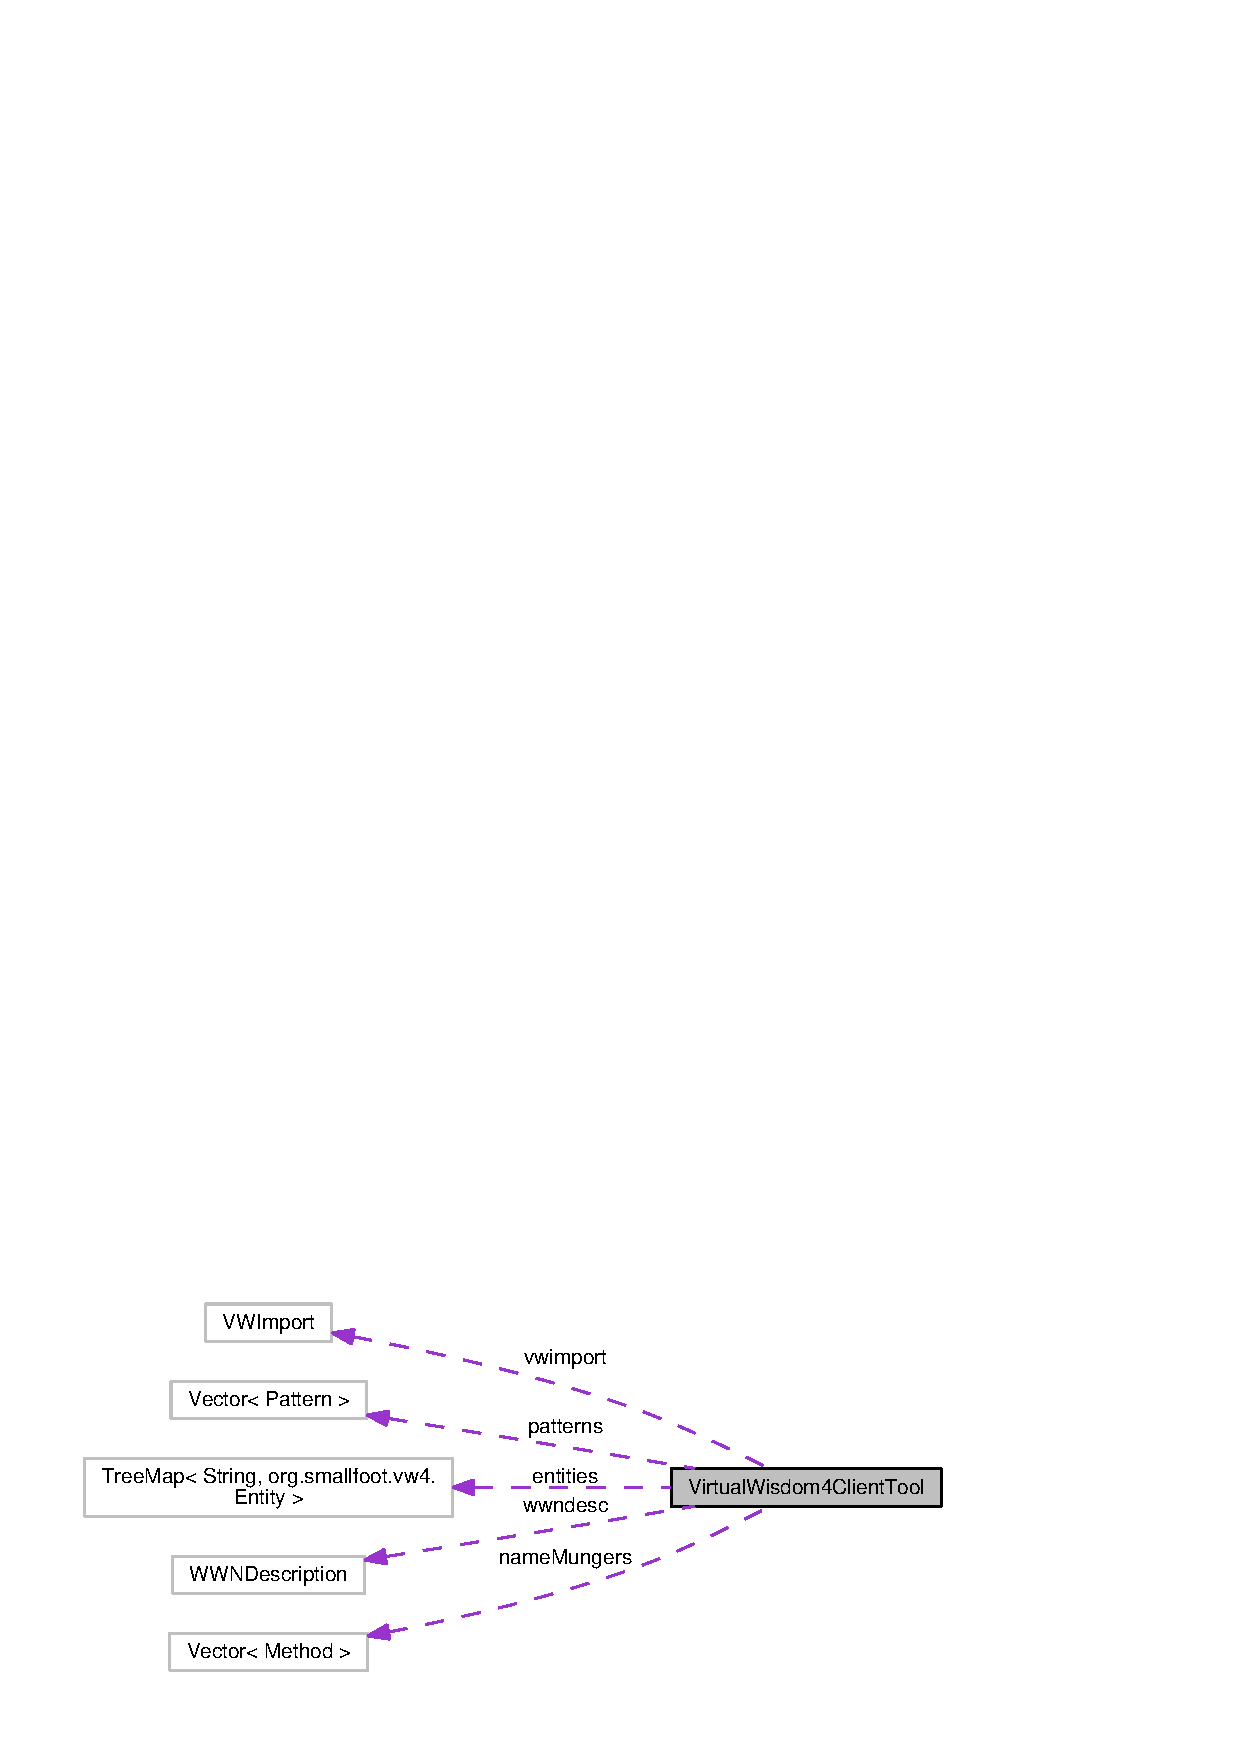
\includegraphics[width=350pt]{classorg_1_1smallfoot_1_1vw4_1_1VirtualWisdom4ClientTool__coll__graph}
\end{center}
\end{figure}
\subsection*{Data Structures}
\begin{DoxyCompactItemize}
\item 
interface {\bf Entity\+Selector}
\begin{DoxyCompactList}\small\item\em simple convenience interface to allow entity selection to be codified and created on-\/the-\/fly in a query A\+P\+I \end{DoxyCompactList}\end{DoxyCompactItemize}
\subsection*{Public Member Functions}
\begin{DoxyCompactItemize}
\item 
{\bf Virtual\+Wisdom4\+Client\+Tool} (String xml\+File)
\begin{DoxyCompactList}\small\item\em Class Constructor to create with an initial file to load. \end{DoxyCompactList}\item 
{\bf Virtual\+Wisdom4\+Client\+Tool} ()\label{classorg_1_1smallfoot_1_1vw4_1_1VirtualWisdom4ClientTool_a7991b30b52ad4d408df3575abc9b57ae}

\begin{DoxyCompactList}\small\item\em Class Constructor with no initial file. \end{DoxyCompactList}\item 
Tree\+Map$<$ String, {\bf Entity} $>$ {\bf entities} ()
\item 
void {\bf load} (String filename)
\begin{DoxyCompactList}\small\item\em Wrapper to just load the file, spitting out exceptions and stacks as they occur. \end{DoxyCompactList}\item 
Vector$<$ Pattern $>$ {\bf patterns} ()
\item 
String {\bf pretty\+J\+S\+O\+N} (V\+W\+Import v)
\begin{DoxyCompactList}\small\item\em Convenience function to generate a pretty-\/printed J\+S\+O\+N text string. \end{DoxyCompactList}\item 
void {\bf save} (String filename)
\begin{DoxyCompactList}\small\item\em Wrapper to just save the file, spitting out exceptions and stacks as they occur. \end{DoxyCompactList}\item 
W\+W\+N\+Description {\bf wwndesc} ()
\end{DoxyCompactItemize}
\subsection*{Static Public Member Functions}
\begin{DoxyCompactItemize}
\item 
static void {\bf main} (String args[$\,$])
\begin{DoxyCompactList}\small\item\em Main function, as you can tell. \end{DoxyCompactList}\end{DoxyCompactItemize}
\subsection*{Data Fields}
\begin{DoxyCompactItemize}
\item 
V\+W\+Import {\bf vwimport} = null\label{classorg_1_1smallfoot_1_1vw4_1_1VirtualWisdom4ClientTool_a4ef055893be8838f513385e4c2f42700}

\begin{DoxyCompactList}\small\item\em singleton list of J\+S\+O\+N-\/writable objects accessed through \doxyref{vwimport()}{p.}{classorg_1_1smallfoot_1_1vw4_1_1VirtualWisdom4ClientTool_acbeee875159f78e186965708e70dee94} \end{DoxyCompactList}\end{DoxyCompactItemize}
\subsection*{Protected Member Functions}
\begin{DoxyCompactItemize}
\item 
void {\bf \+\_\+load} (String filename)  throws java.\+io.\+I\+O\+Exception     
\begin{DoxyCompactList}\small\item\em Open a file. \end{DoxyCompactList}\item 
void {\bf \+\_\+save} (String filename)  throws java.\+lang.\+Exception     
\begin{DoxyCompactList}\small\item\em Save the current X\+M\+L Document to a new file. \end{DoxyCompactList}\item 
void {\bf load\+And\+Absorb\+File} (String f)
\begin{DoxyCompactList}\small\item\em one-\/shot load a new file and absorb the contents\+: open the file and stream the contents at an array of parsers, the one with the best results wins; using that result, absorb all alias information, attempting to create parent storagecontroller(s) or hosts as resulting from absorbtion patterns \end{DoxyCompactList}\item 
void {\bf load\+And\+Remove\+File} (String f)
\begin{DoxyCompactList}\small\item\em one-\/shot load a new file and remove the contents from the internal list of leaf\+Entities (H\+B\+As, F\+As) \end{DoxyCompactList}\item 
V\+W\+Import {\bf vwimport} ()
\end{DoxyCompactItemize}
\subsection*{Protected Attributes}
\begin{DoxyCompactItemize}
\item 
Tree\+Map$<$ String, {\bf Entity} $>$ {\bf entities} = null\label{classorg_1_1smallfoot_1_1vw4_1_1VirtualWisdom4ClientTool_ac3c495e48cdbca229137371be08ba04f}

\begin{DoxyCompactList}\small\item\em local singleton array accessed from \doxyref{entities()}{p.}{classorg_1_1smallfoot_1_1vw4_1_1VirtualWisdom4ClientTool_aa9ab77e799e869cf9da3d339e124f6c4} \end{DoxyCompactList}\item 
Vector$<$ Pattern $>$ {\bf patterns} = null\label{classorg_1_1smallfoot_1_1vw4_1_1VirtualWisdom4ClientTool_aaa7580a75c1bf3c122ce5b4c001517c2}

\begin{DoxyCompactList}\small\item\em local singleton array accessed from \doxyref{patterns()}{p.}{classorg_1_1smallfoot_1_1vw4_1_1VirtualWisdom4ClientTool_a09f298d19a33be899f5835657c747c5d} \end{DoxyCompactList}\item 
W\+W\+N\+Description {\bf wwndesc} = null\label{classorg_1_1smallfoot_1_1vw4_1_1VirtualWisdom4ClientTool_afb3f7acf97044713e2aa55c921c5cdb2}

\begin{DoxyCompactList}\small\item\em local singleton array accessed from \doxyref{wwndesc()}{p.}{classorg_1_1smallfoot_1_1vw4_1_1VirtualWisdom4ClientTool_a43a8de962936ee9d82e0a70eeb9b1db6} \end{DoxyCompactList}\end{DoxyCompactItemize}
\subsection*{Private Attributes}
\begin{DoxyCompactItemize}
\item 
org.\+w3c.\+dom.\+Document {\bf xml\+Document}\label{classorg_1_1smallfoot_1_1vw4_1_1VirtualWisdom4ClientTool_ad25ef6220eb54575157ab063bc63a0f0}

\begin{DoxyCompactList}\small\item\em eventually used to hold an X\+M\+L document when converting X\+M\+L$<$--$>$J\+S\+O\+N$<$--$>$X\+M\+L \end{DoxyCompactList}\end{DoxyCompactItemize}


\subsection{Detailed Description}
\doxyref{Virtual\+Wisdom4\+Client\+Tool}{p.}{classorg_1_1smallfoot_1_1vw4_1_1VirtualWisdom4ClientTool} is a \char`\"{}\+Swiss Army Knife\char`\"{} of tools used when working with Virtual\+Wisdom4. 

The existence of these tools is not a judgement on Virtual\+Wisdom4's proper Engineering; rather, an acceptance that a faster-\/response solution for the longer-\/tail of the normal curve is often helpful swapping Q\+A delay for reduced customer friction.

As you'd expect, there is no support for this. If it breaks, you may choose to keep both pieces \+:)

Ad-\/\+Hoc content for this utility-\/stack may appear at {\tt http\+://fcfae.\+com/} 

Definition at line 56 of file Virtual\+Wisdom4\+Client\+Tool.\+java.



\subsection{Constructor \& Destructor Documentation}
\index{org\+::smallfoot\+::vw4\+::\+Virtual\+Wisdom4\+Client\+Tool@{org\+::smallfoot\+::vw4\+::\+Virtual\+Wisdom4\+Client\+Tool}!Virtual\+Wisdom4\+Client\+Tool@{Virtual\+Wisdom4\+Client\+Tool}}
\index{Virtual\+Wisdom4\+Client\+Tool@{Virtual\+Wisdom4\+Client\+Tool}!org\+::smallfoot\+::vw4\+::\+Virtual\+Wisdom4\+Client\+Tool@{org\+::smallfoot\+::vw4\+::\+Virtual\+Wisdom4\+Client\+Tool}}
\subsubsection[{Virtual\+Wisdom4\+Client\+Tool}]{\setlength{\rightskip}{0pt plus 5cm}{\bf Virtual\+Wisdom4\+Client\+Tool} (
\begin{DoxyParamCaption}
\item[{String}]{xml\+File}
\end{DoxyParamCaption}
)\hspace{0.3cm}{\ttfamily [inline]}}\label{classorg_1_1smallfoot_1_1vw4_1_1VirtualWisdom4ClientTool_a0f1b4c518fafff8a296bb632e57655ca}


Class Constructor to create with an initial file to load. 


\begin{DoxyParams}{Parameters}
{\em xml\+File} & File to load at start\\
\hline
\end{DoxyParams}
\begin{DoxySeeAlso}{See also}
\doxyref{load(\+String)}{p.}{classorg_1_1smallfoot_1_1vw4_1_1VirtualWisdom4ClientTool_a0d686f1044a2e8727b12e6e4921e0e8f} 
\end{DoxySeeAlso}


Definition at line 67 of file Virtual\+Wisdom4\+Client\+Tool.\+java.



References Virtual\+Wisdom4\+Client\+Tool.\+load().



Here is the call graph for this function\+:\nopagebreak
\begin{figure}[H]
\begin{center}
\leavevmode
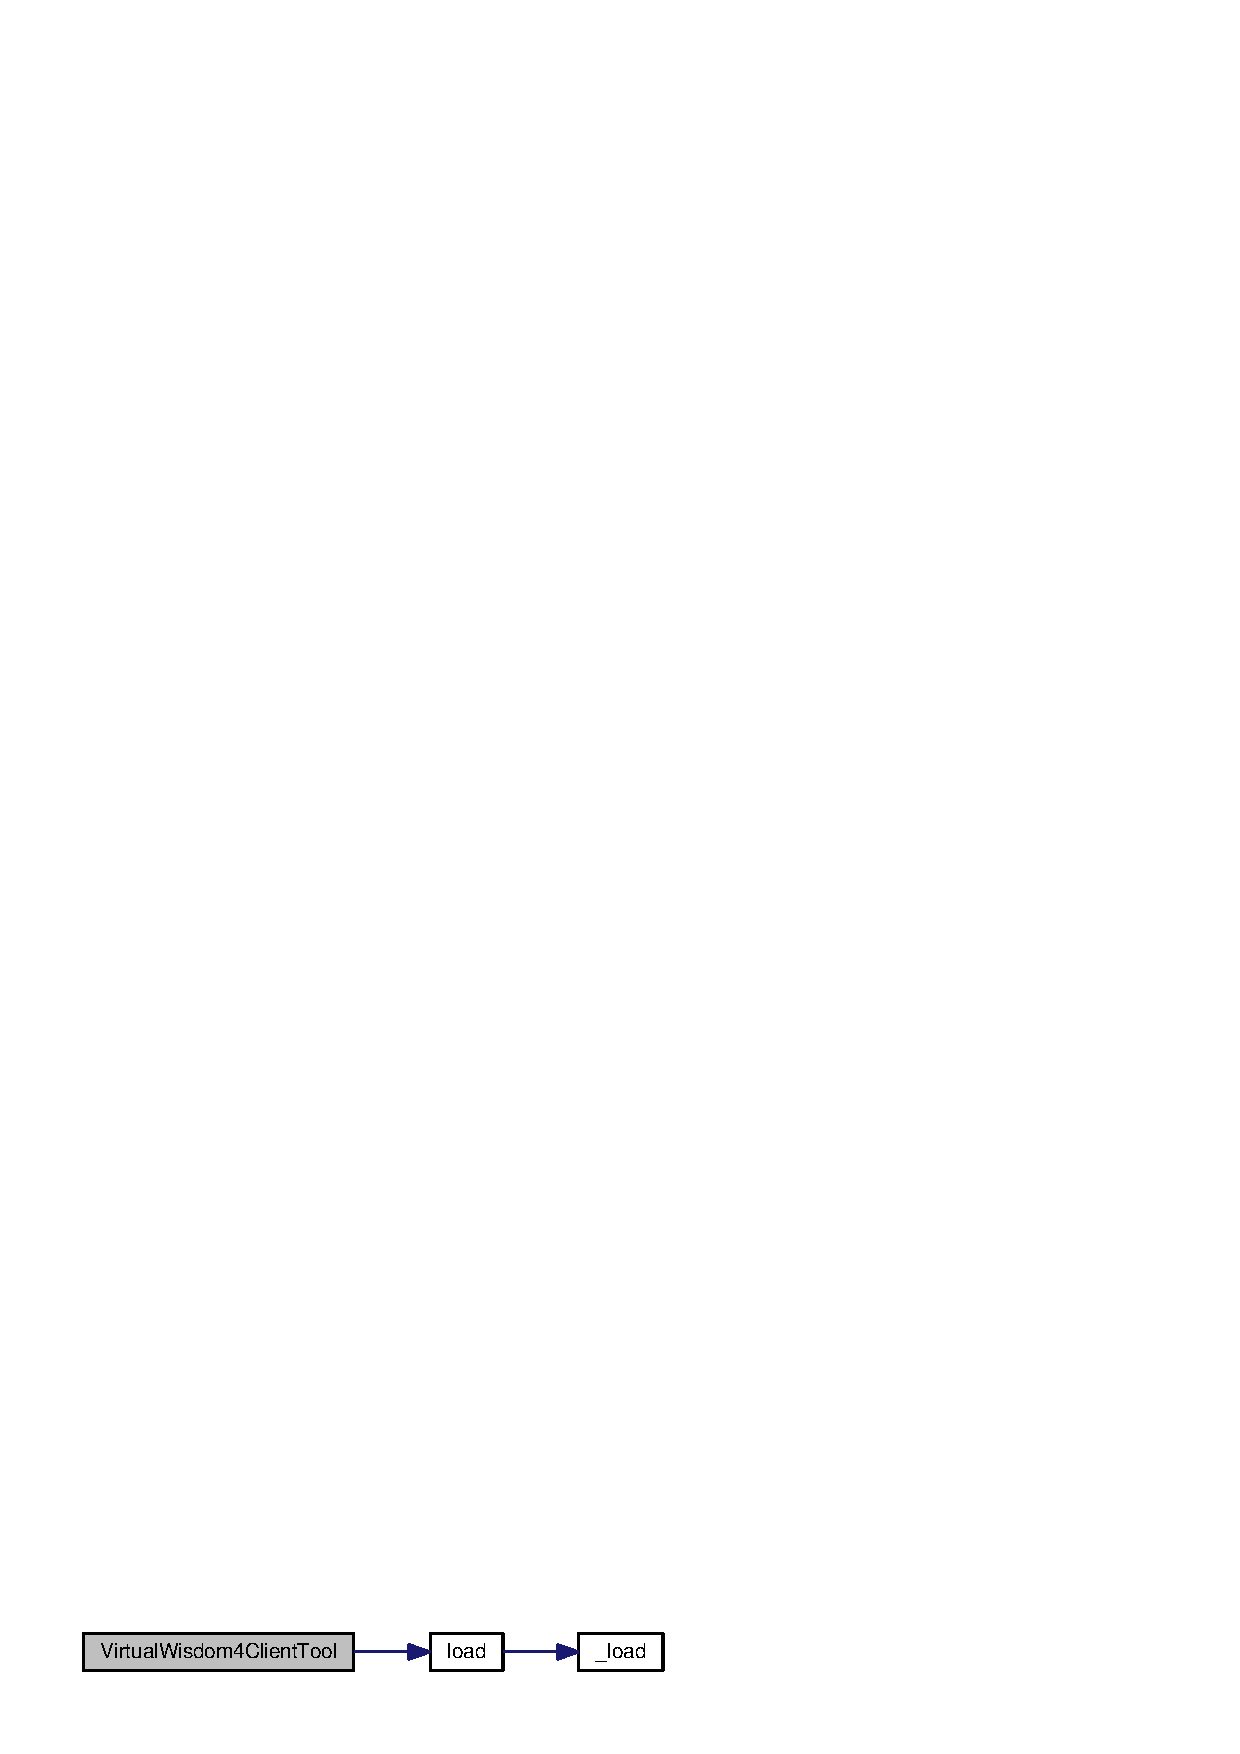
\includegraphics[width=322pt]{classorg_1_1smallfoot_1_1vw4_1_1VirtualWisdom4ClientTool_a0f1b4c518fafff8a296bb632e57655ca_cgraph}
\end{center}
\end{figure}




\subsection{Member Function Documentation}
\index{org\+::smallfoot\+::vw4\+::\+Virtual\+Wisdom4\+Client\+Tool@{org\+::smallfoot\+::vw4\+::\+Virtual\+Wisdom4\+Client\+Tool}!\+\_\+load@{\+\_\+load}}
\index{\+\_\+load@{\+\_\+load}!org\+::smallfoot\+::vw4\+::\+Virtual\+Wisdom4\+Client\+Tool@{org\+::smallfoot\+::vw4\+::\+Virtual\+Wisdom4\+Client\+Tool}}
\subsubsection[{\+\_\+load}]{\setlength{\rightskip}{0pt plus 5cm}void \+\_\+load (
\begin{DoxyParamCaption}
\item[{String}]{filename}
\end{DoxyParamCaption}
) throws java.\+io.\+I\+O\+Exception\hspace{0.3cm}{\ttfamily [inline]}, {\ttfamily [protected]}}\label{classorg_1_1smallfoot_1_1vw4_1_1VirtualWisdom4ClientTool_ad9a051ba608e7fcb9adac39bc3946058}


Open a file. 

This is actually a wrapper for the underlying file load


\begin{DoxyParams}{Parameters}
{\em filename} & file to load \\
\hline
\end{DoxyParams}

\begin{DoxyExceptions}{Exceptions}
{\em I\+O\+Exception} & when File() encounters an error instaitating (typically path or permissions) \\
\hline
\end{DoxyExceptions}
\begin{DoxyRefDesc}{Todo}
\item[{\bf Todo}]\+: evaluate\+: mapper.\+configure(Deserialization\+Config.\+Feature.\+F\+A\+I\+L\+\_\+\+O\+N\+\_\+\+U\+N\+K\+N\+O\+W\+N\+\_\+\+P\+R\+O\+P\+E\+R\+T\+I\+E\+S, false); \end{DoxyRefDesc}


Definition at line 96 of file Virtual\+Wisdom4\+Client\+Tool.\+java.



Referenced by Virtual\+Wisdom4\+Client\+Tool.\+load().

\index{org\+::smallfoot\+::vw4\+::\+Virtual\+Wisdom4\+Client\+Tool@{org\+::smallfoot\+::vw4\+::\+Virtual\+Wisdom4\+Client\+Tool}!\+\_\+save@{\+\_\+save}}
\index{\+\_\+save@{\+\_\+save}!org\+::smallfoot\+::vw4\+::\+Virtual\+Wisdom4\+Client\+Tool@{org\+::smallfoot\+::vw4\+::\+Virtual\+Wisdom4\+Client\+Tool}}
\subsubsection[{\+\_\+save}]{\setlength{\rightskip}{0pt plus 5cm}void \+\_\+save (
\begin{DoxyParamCaption}
\item[{String}]{filename}
\end{DoxyParamCaption}
) throws java.\+lang.\+Exception\hspace{0.3cm}{\ttfamily [inline]}, {\ttfamily [protected]}}\label{classorg_1_1smallfoot_1_1vw4_1_1VirtualWisdom4ClientTool_a36a7decd28b5e191bfe43c5562462785}


Save the current X\+M\+L Document to a new file. 


\begin{DoxyParams}{Parameters}
{\em filename} & filename to save into \\
\hline
\end{DoxyParams}


Definition at line 131 of file Virtual\+Wisdom4\+Client\+Tool.\+java.



Referenced by Virtual\+Wisdom4\+Client\+Tool.\+save().

\index{org\+::smallfoot\+::vw4\+::\+Virtual\+Wisdom4\+Client\+Tool@{org\+::smallfoot\+::vw4\+::\+Virtual\+Wisdom4\+Client\+Tool}!entities@{entities}}
\index{entities@{entities}!org\+::smallfoot\+::vw4\+::\+Virtual\+Wisdom4\+Client\+Tool@{org\+::smallfoot\+::vw4\+::\+Virtual\+Wisdom4\+Client\+Tool}}
\subsubsection[{entities}]{\setlength{\rightskip}{0pt plus 5cm}Tree\+Map$<$String,{\bf Entity}$>$ entities (
\begin{DoxyParamCaption}
{}
\end{DoxyParamCaption}
)\hspace{0.3cm}{\ttfamily [inline]}}\label{classorg_1_1smallfoot_1_1vw4_1_1VirtualWisdom4ClientTool_aa9ab77e799e869cf9da3d339e124f6c4}
$<$ singleton access for entities \begin{DoxyReturn}{Returns}
collection of entities 
\end{DoxyReturn}


Definition at line 194 of file Virtual\+Wisdom4\+Client\+Tool.\+java.



Referenced by Virtual\+Wisdom4\+Client\+Tool.\+load\+And\+Absorb\+File().

\index{org\+::smallfoot\+::vw4\+::\+Virtual\+Wisdom4\+Client\+Tool@{org\+::smallfoot\+::vw4\+::\+Virtual\+Wisdom4\+Client\+Tool}!load@{load}}
\index{load@{load}!org\+::smallfoot\+::vw4\+::\+Virtual\+Wisdom4\+Client\+Tool@{org\+::smallfoot\+::vw4\+::\+Virtual\+Wisdom4\+Client\+Tool}}
\subsubsection[{load}]{\setlength{\rightskip}{0pt plus 5cm}void load (
\begin{DoxyParamCaption}
\item[{String}]{filename}
\end{DoxyParamCaption}
)\hspace{0.3cm}{\ttfamily [inline]}}\label{classorg_1_1smallfoot_1_1vw4_1_1VirtualWisdom4ClientTool_a0d686f1044a2e8727b12e6e4921e0e8f}


Wrapper to just load the file, spitting out exceptions and stacks as they occur. 


\begin{DoxyParams}{Parameters}
{\em filename} & file to load \\
\hline
\end{DoxyParams}


Definition at line 110 of file Virtual\+Wisdom4\+Client\+Tool.\+java.



References Virtual\+Wisdom4\+Client\+Tool.\+\_\+load().



Referenced by Virtual\+Wisdom4\+Client\+Tool.\+main(), and Virtual\+Wisdom4\+Client\+Tool.\+Virtual\+Wisdom4\+Client\+Tool().



Here is the call graph for this function\+:\nopagebreak
\begin{figure}[H]
\begin{center}
\leavevmode
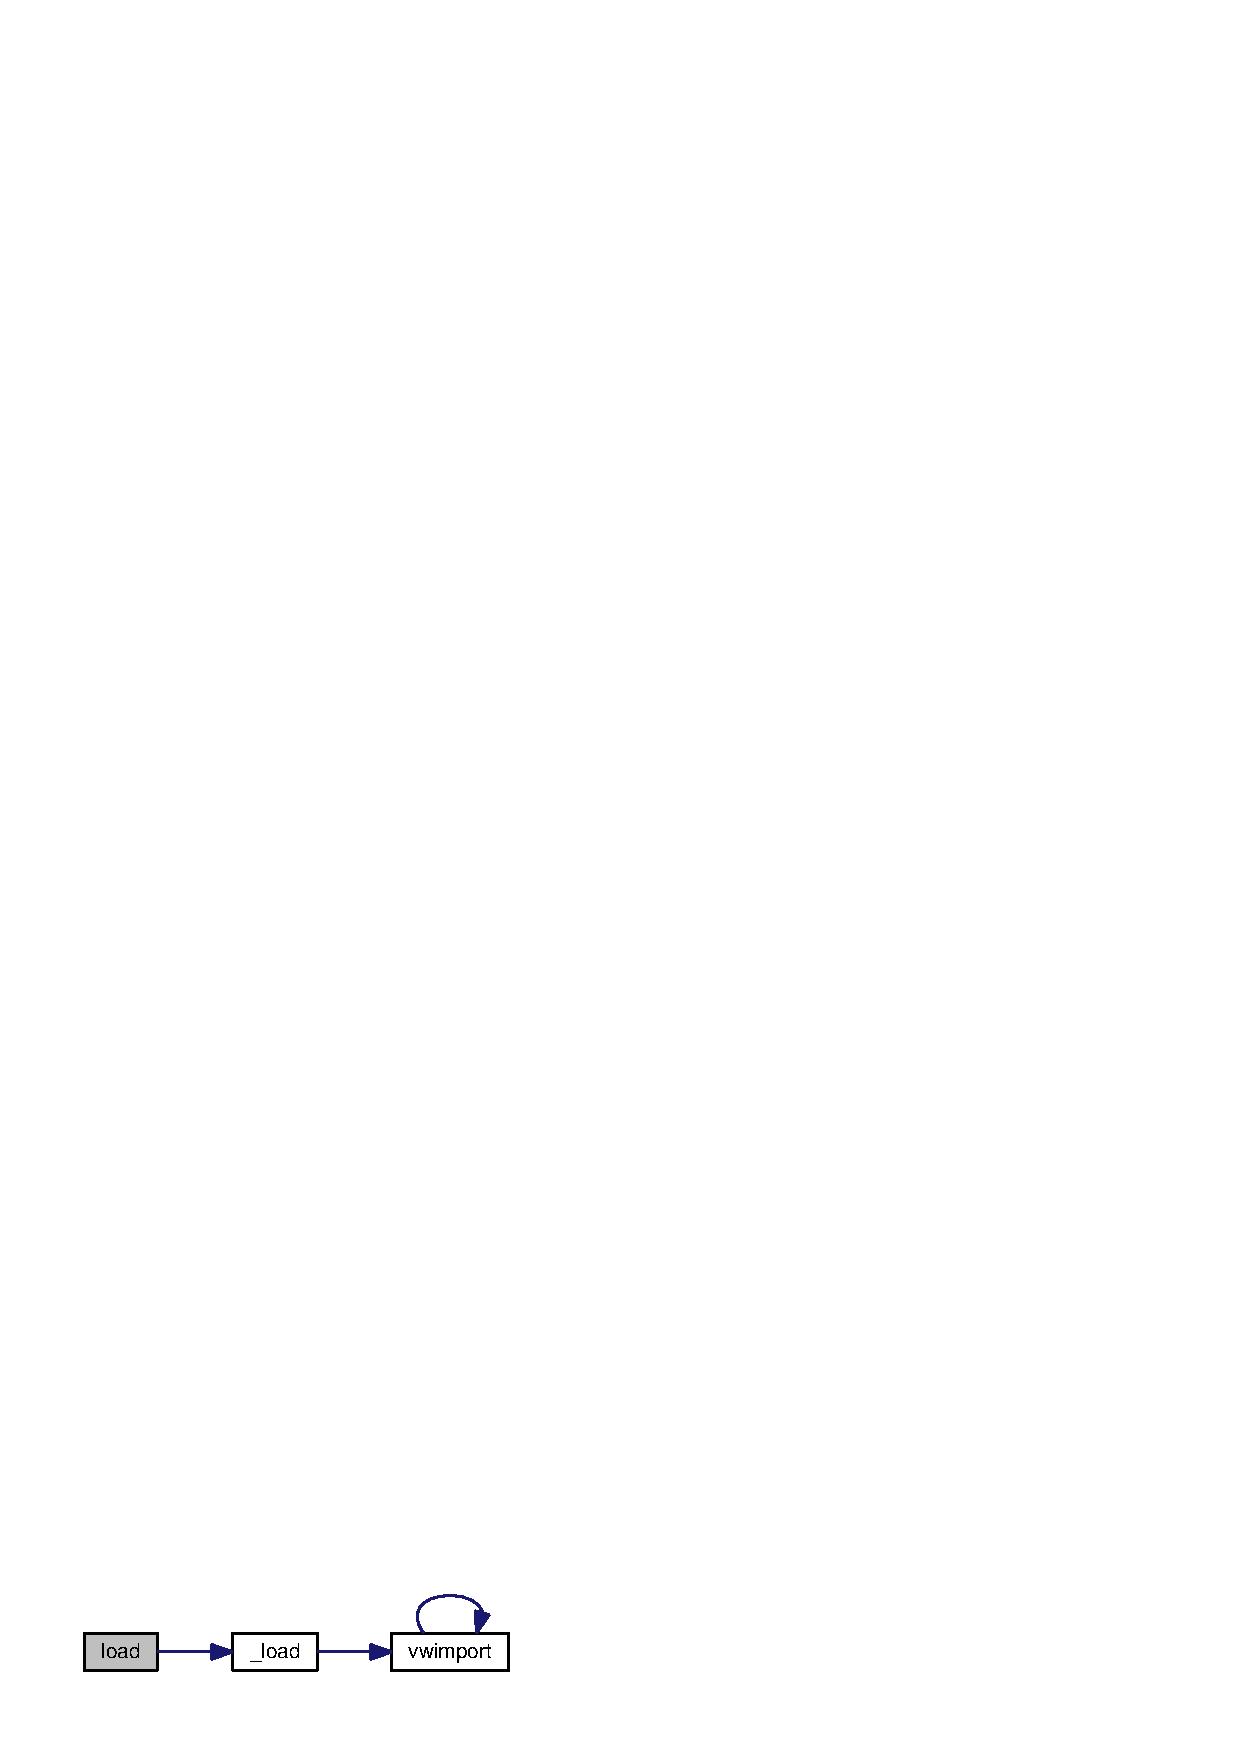
\includegraphics[width=156pt]{classorg_1_1smallfoot_1_1vw4_1_1VirtualWisdom4ClientTool_a0d686f1044a2e8727b12e6e4921e0e8f_cgraph}
\end{center}
\end{figure}


\index{org\+::smallfoot\+::vw4\+::\+Virtual\+Wisdom4\+Client\+Tool@{org\+::smallfoot\+::vw4\+::\+Virtual\+Wisdom4\+Client\+Tool}!load\+And\+Absorb\+File@{load\+And\+Absorb\+File}}
\index{load\+And\+Absorb\+File@{load\+And\+Absorb\+File}!org\+::smallfoot\+::vw4\+::\+Virtual\+Wisdom4\+Client\+Tool@{org\+::smallfoot\+::vw4\+::\+Virtual\+Wisdom4\+Client\+Tool}}
\subsubsection[{load\+And\+Absorb\+File}]{\setlength{\rightskip}{0pt plus 5cm}void load\+And\+Absorb\+File (
\begin{DoxyParamCaption}
\item[{String}]{f}
\end{DoxyParamCaption}
)\hspace{0.3cm}{\ttfamily [inline]}, {\ttfamily [protected]}}\label{classorg_1_1smallfoot_1_1vw4_1_1VirtualWisdom4ClientTool_a36539eb2d98fcdcedd7dc2088acfeef2}


one-\/shot load a new file and absorb the contents\+: open the file and stream the contents at an array of parsers, the one with the best results wins; using that result, absorb all alias information, attempting to create parent storagecontroller(s) or hosts as resulting from absorbtion patterns 


\begin{DoxyParams}{Parameters}
{\em f} & name of file to open\\
\hline
\end{DoxyParams}
\begin{DoxySeeAlso}{See also}
{\tt https\+://github.\+com/chickenandpork/fibrechannel-\/parsers/} 
\end{DoxySeeAlso}


Definition at line 497 of file Virtual\+Wisdom4\+Client\+Tool.\+java.



References Virtual\+Wisdom4\+Client\+Tool.\+entities(), Entity.\+name, Entity.\+set\+Description(), Entity.\+setname(), and Virtual\+Wisdom4\+Client\+Tool.\+wwndesc().



Referenced by Virtual\+Wisdom4\+Client\+Tool.\+main().



Here is the call graph for this function\+:\nopagebreak
\begin{figure}[H]
\begin{center}
\leavevmode
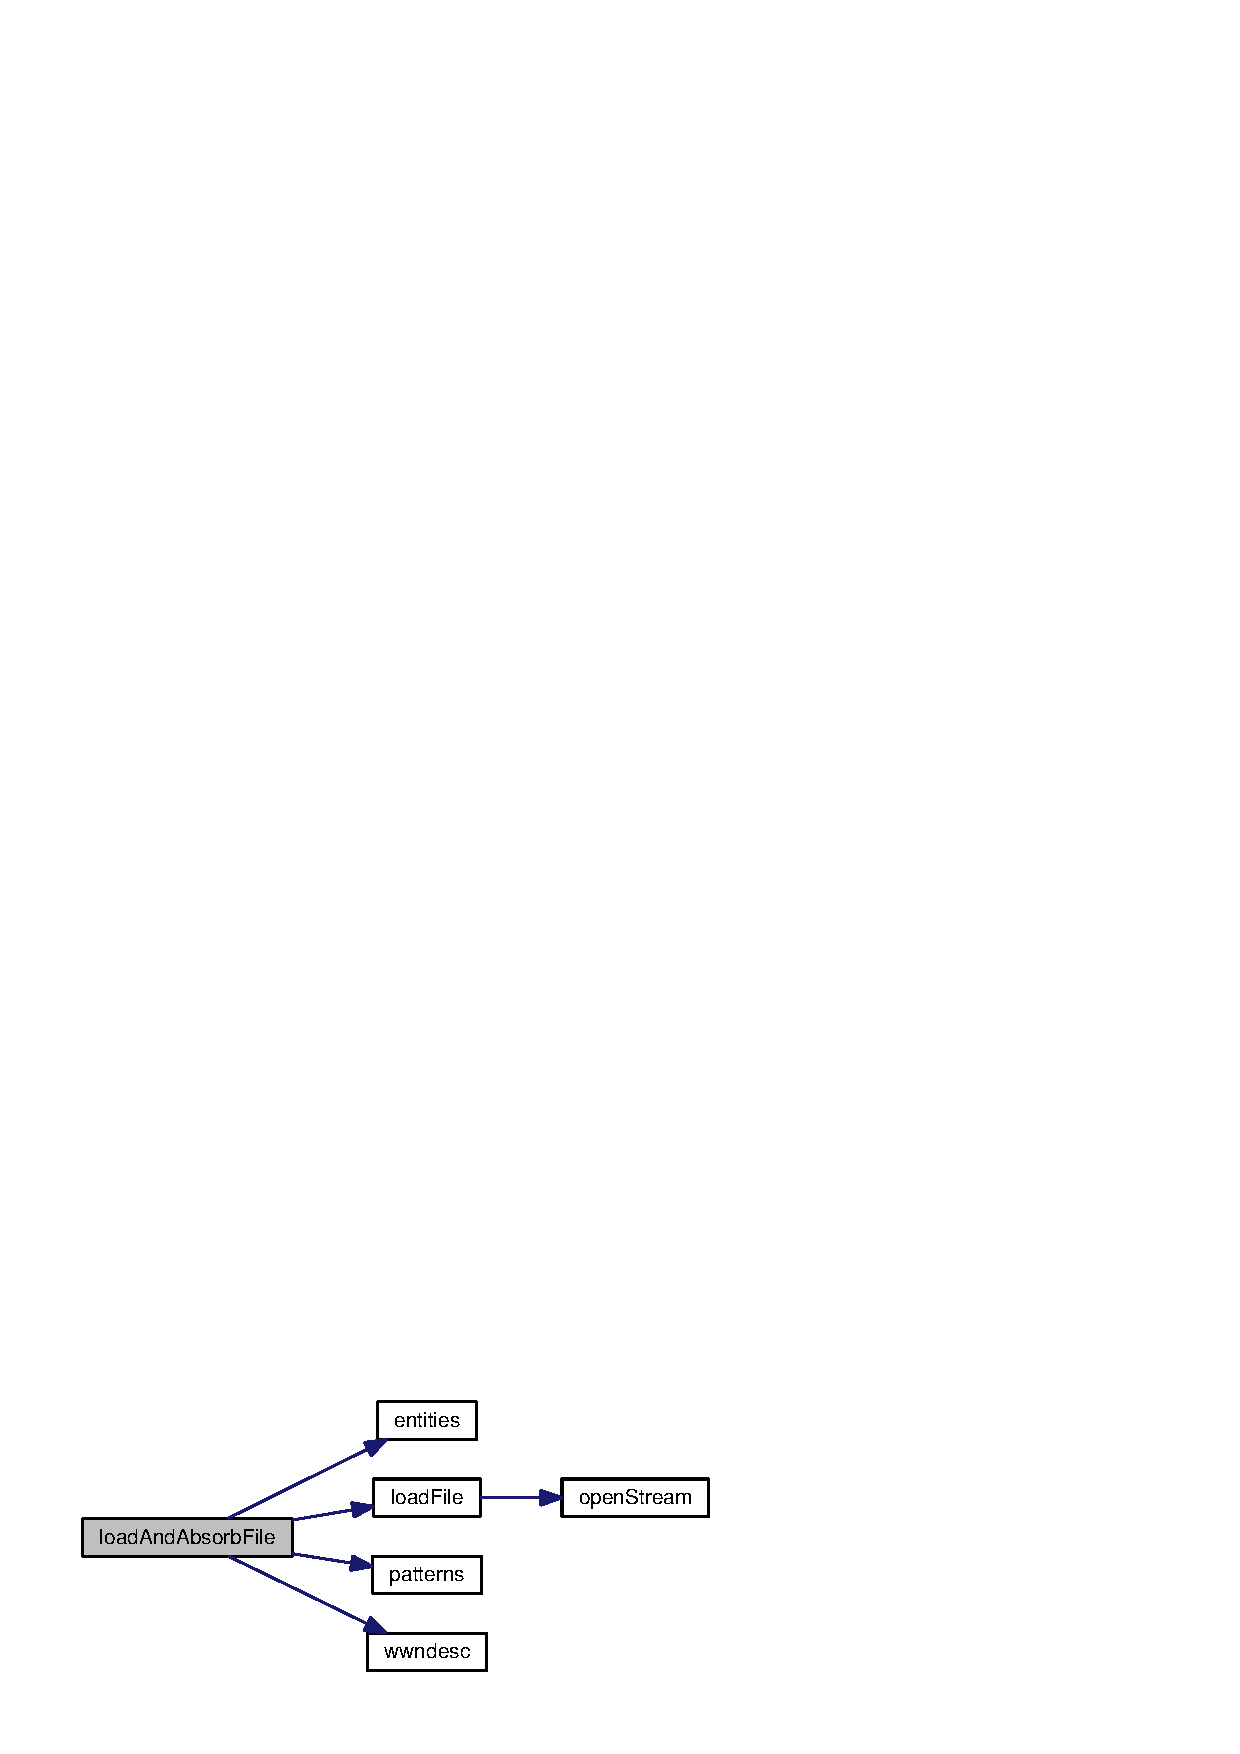
\includegraphics[width=350pt]{classorg_1_1smallfoot_1_1vw4_1_1VirtualWisdom4ClientTool_a36539eb2d98fcdcedd7dc2088acfeef2_cgraph}
\end{center}
\end{figure}


\index{org\+::smallfoot\+::vw4\+::\+Virtual\+Wisdom4\+Client\+Tool@{org\+::smallfoot\+::vw4\+::\+Virtual\+Wisdom4\+Client\+Tool}!load\+And\+Remove\+File@{load\+And\+Remove\+File}}
\index{load\+And\+Remove\+File@{load\+And\+Remove\+File}!org\+::smallfoot\+::vw4\+::\+Virtual\+Wisdom4\+Client\+Tool@{org\+::smallfoot\+::vw4\+::\+Virtual\+Wisdom4\+Client\+Tool}}
\subsubsection[{load\+And\+Remove\+File}]{\setlength{\rightskip}{0pt plus 5cm}void load\+And\+Remove\+File (
\begin{DoxyParamCaption}
\item[{String}]{f}
\end{DoxyParamCaption}
)\hspace{0.3cm}{\ttfamily [inline]}, {\ttfamily [protected]}}\label{classorg_1_1smallfoot_1_1vw4_1_1VirtualWisdom4ClientTool_a2e5ab2ec8715ec815edcea74375a493c}


one-\/shot load a new file and remove the contents from the internal list of leaf\+Entities (H\+B\+As, F\+As) 

Working on only the leaf entities, this uses the parser array to parse an input stream, and for each W\+W\+P\+N found, it removes that leaf entity from the system. It doesn't affect the child\+\_\+entities of referring entities to allow for a loaded entity list to still refer to entities which are already on the target system.


\begin{DoxyParams}{Parameters}
{\em f} & name of file to open\\
\hline
\end{DoxyParams}
\begin{DoxySeeAlso}{See also}
{\tt https\+://github.\+com/chickenandpork/fibrechannel-\/parsers/} 
\end{DoxySeeAlso}


Definition at line 433 of file Virtual\+Wisdom4\+Client\+Tool.\+java.



Referenced by Virtual\+Wisdom4\+Client\+Tool.\+main().

\index{org\+::smallfoot\+::vw4\+::\+Virtual\+Wisdom4\+Client\+Tool@{org\+::smallfoot\+::vw4\+::\+Virtual\+Wisdom4\+Client\+Tool}!main@{main}}
\index{main@{main}!org\+::smallfoot\+::vw4\+::\+Virtual\+Wisdom4\+Client\+Tool@{org\+::smallfoot\+::vw4\+::\+Virtual\+Wisdom4\+Client\+Tool}}
\subsubsection[{main}]{\setlength{\rightskip}{0pt plus 5cm}static void main (
\begin{DoxyParamCaption}
\item[{String}]{args[$\,$]}
\end{DoxyParamCaption}
)\hspace{0.3cm}{\ttfamily [inline]}, {\ttfamily [static]}}\label{classorg_1_1smallfoot_1_1vw4_1_1VirtualWisdom4ClientTool_a75988cf84fc6ee7a2ebff36e363021aa}


Main function, as you can tell. 

this function merely parses the command-\/line to dispatch actions to the meat of the meal above. I'm using an actual Get\+Opt because, yes, I'm a U\+N\+I\+X/\+C hack, re-\/using 3-\/decades-\/old knowledge, but this also preserves both extensibility and the ability to use longopts in scripts as a way to self-\/document what the tool's doing.

No real intelligence herein except the parse-\/and-\/redirect action.


\begin{DoxyParams}{Parameters}
{\em args} & as you'd expect, these are commandline arguments given when the jar is activated \\
\hline
\end{DoxyParams}
Always always A\+L\+W\+A\+Y\+S provide a quick reference and a version output

\begin{DoxyRefDesc}{Commandline Options}
\item[{\bf Commandline Options}]-\/\+H$\vert$--help Show a simple help screen as a reminder of options which are understood by the application \end{DoxyRefDesc}
\begin{DoxyRefDesc}{Commandline Options}
\item[{\bf Commandline Options}]
\begin{DoxyCode}
java -jar vw4tools.jar --help 
\end{DoxyCode}
\end{DoxyRefDesc}


\begin{DoxyRefDesc}{Commandline Options}
\item[{\bf Commandline Options}]-\/\+V$\vert$--version Show the current release version for reference \end{DoxyRefDesc}
\begin{DoxyRefDesc}{Commandline Options}
\item[{\bf Commandline Options}]
\begin{DoxyCode}
java -jar vw4tools.jar --version
 0.9-94 
\end{DoxyCode}
\end{DoxyRefDesc}


\begin{DoxyRefDesc}{Commandline Options}
\item[{\bf Commandline Options}]-\/n$\vert$--nicknameout=\{file\} Output nicknames from internal store \end{DoxyRefDesc}
\begin{DoxyRefDesc}{Commandline Options}
\item[{\bf Commandline Options}]-\/o$\vert$--output=\{file\} Output nicknames from internal store --nicknameout and --output are currently functionally identical; they both cause the internal nickname/entity base to be written out as J\+S\+O\+N with the exception of a few \char`\"{}magic\char`\"{} filenames\+:\end{DoxyRefDesc}


\begin{DoxyRefDesc}{Commandline Options}
\item[{\bf Commandline Options}]
\begin{DoxyEnumerate}
\item {\bfseries schema.\+json} will cause the current schema to be written 
\end{DoxyEnumerate}\end{DoxyRefDesc}
\begin{DoxyRefDesc}{Commandline Options}
\item[{\bf Commandline Options}]
\begin{DoxyEnumerate}
\item {\bfseries orderedtuples.\+csv} will cause an Ordered\+Tuples.\+csv file to be written, suitable for post-\/processing via \doxyref{csv-\/to-\/json.\+awk}{p.}{csv-to-json_8awk} but allowing a user to more easily edit C\+S\+V for fine-\/tuning 
\end{DoxyEnumerate}\end{DoxyRefDesc}
\begin{DoxyRefDesc}{Commandline Options}
\item[{\bf Commandline Options}]
\begin{DoxyEnumerate}
\item {\bfseries orphanentities.\+csv} will cause a C\+S\+V to be written listing all orphan entities. An \char`\"{}\+Orphan Entity\char`\"{} is an entity lacking a parent entity, such as an \char`\"{}\+H\+B\+A Port\char`\"{} without a \char`\"{}host\char`\"{} parent, or a \char`\"{}iomodule\char`\"{} without a parent \char`\"{}storagearray\char`\"{} entity.
\end{DoxyEnumerate}\end{DoxyRefDesc}


\begin{DoxyRefDesc}{Commandline Options}
\item[{\bf Commandline Options}]All other filename patterns will result in a J\+S\+O\+N-\/formatted file\end{DoxyRefDesc}


\begin{DoxyRefDesc}{Commandline Options}
\item[{\bf Commandline Options}]-\/\+N$\vert$--nickname=\{file/uri\} Import nicknames by parsing a text stream from various sources \end{DoxyRefDesc}
\begin{DoxyRefDesc}{Commandline Options}
\item[{\bf Commandline Options}]
\begin{DoxyCode}
java -jar vw4tools.jar --nickname=switch44.zoneshow
      Parse results \textcolor{keywordflow}{for} AliShowZoneParser:
      Zones: 44
      Aliases: 112 (names with one or more WWPNs)
      Aliases: 136 (name/WWPN tuples) 
\end{DoxyCode}
 In this example, a zone file was parsed by the Ali\+Show\+Zone\+Parser resulting in 112 nicknames; due to duplicate nicknames, there are actually 136 unique W\+W\+P\+N/alias tuples, which means that (136-\/112) 24 of the W\+W\+P\+Ns have the same alias as other W\+W\+P\+Ns\end{DoxyRefDesc}


\begin{DoxyRefDesc}{Commandline Options}
\item[{\bf Commandline Options}]-\/i$\vert$--input import an existing J\+S\+O\+N file for later editing \end{DoxyRefDesc}
\begin{DoxyRefDesc}{Commandline Options}
\item[{\bf Commandline Options}]-\/r$\vert$--read import an existing J\+S\+O\+N file for later editing \end{DoxyRefDesc}
\begin{DoxyRefDesc}{Commandline Options}
\item[{\bf Commandline Options}]
\begin{DoxyCode}
java -jar vw4tools.jar --read working.json 
\end{DoxyCode}
\end{DoxyRefDesc}


\begin{DoxyRefDesc}{Commandline Options}
\item[{\bf Commandline Options}]-\/\+R$\vert$--remove Parse ncknames for removal from the internal nickname list \end{DoxyRefDesc}
\begin{DoxyRefDesc}{Commandline Options}
\item[{\bf Commandline Options}]-\/\+R$\vert$--removenicknames Parse ncknames for removal from the internal nickname list\end{DoxyRefDesc}


\begin{DoxyRefDesc}{Commandline Options}
\item[{\bf Commandline Options}]-\/!$\vert$--report Summarize the current status of the internal nicknaes and pattern/collation coverage \end{DoxyRefDesc}
\begin{DoxyRefDesc}{Commandline Options}
\item[{\bf Commandline Options}]
\begin{DoxyCode}
java -jar vw4tools.jar --nickname=switch44.zoneshow  --report
(vw4tools) parsed 0 zones, 2 aliases via Alias4Parser
vw4tools 0.9-94
    5 total entities
    4 leaf nodes
    2 orphans
50.00 % coverage 
\end{DoxyCode}
 \end{DoxyRefDesc}


\begin{DoxyRefDesc}{Commandline Options}
\item[{\bf Commandline Options}]-\/\+P$\vert$--pattern= is used to provide an \char`\"{}aggregating pattern\char`\"{} to collect Orphan Entities into a container. An \char`\"{}\+Orphan Entity\char`\"{} is an entity which is not part of a larger device\+: an H\+B\+A not assigned to a host, or a F\+A not assigned to a storage array. Aggregating Patterns are evaluated immediately, so their order amidst other command options to import or remove entities is important. \end{DoxyRefDesc}


Definition at line 757 of file Virtual\+Wisdom4\+Client\+Tool.\+java.



References Entity.\+description, Virtual\+Wisdom4\+Client\+Tool.\+entities, Virtual\+Wisdom4\+Client\+Tool.\+load(), Virtual\+Wisdom4\+Client\+Tool.\+load\+And\+Absorb\+File(), Virtual\+Wisdom4\+Client\+Tool.\+load\+And\+Remove\+File(), Entity.\+name, Virtual\+Wisdom4\+Client\+Tool.\+Virtual\+Wisdom4\+Client\+Tool(), and Virtual\+Wisdom4\+Client\+Tool.\+vwimport.



Here is the call graph for this function\+:\nopagebreak
\begin{figure}[H]
\begin{center}
\leavevmode
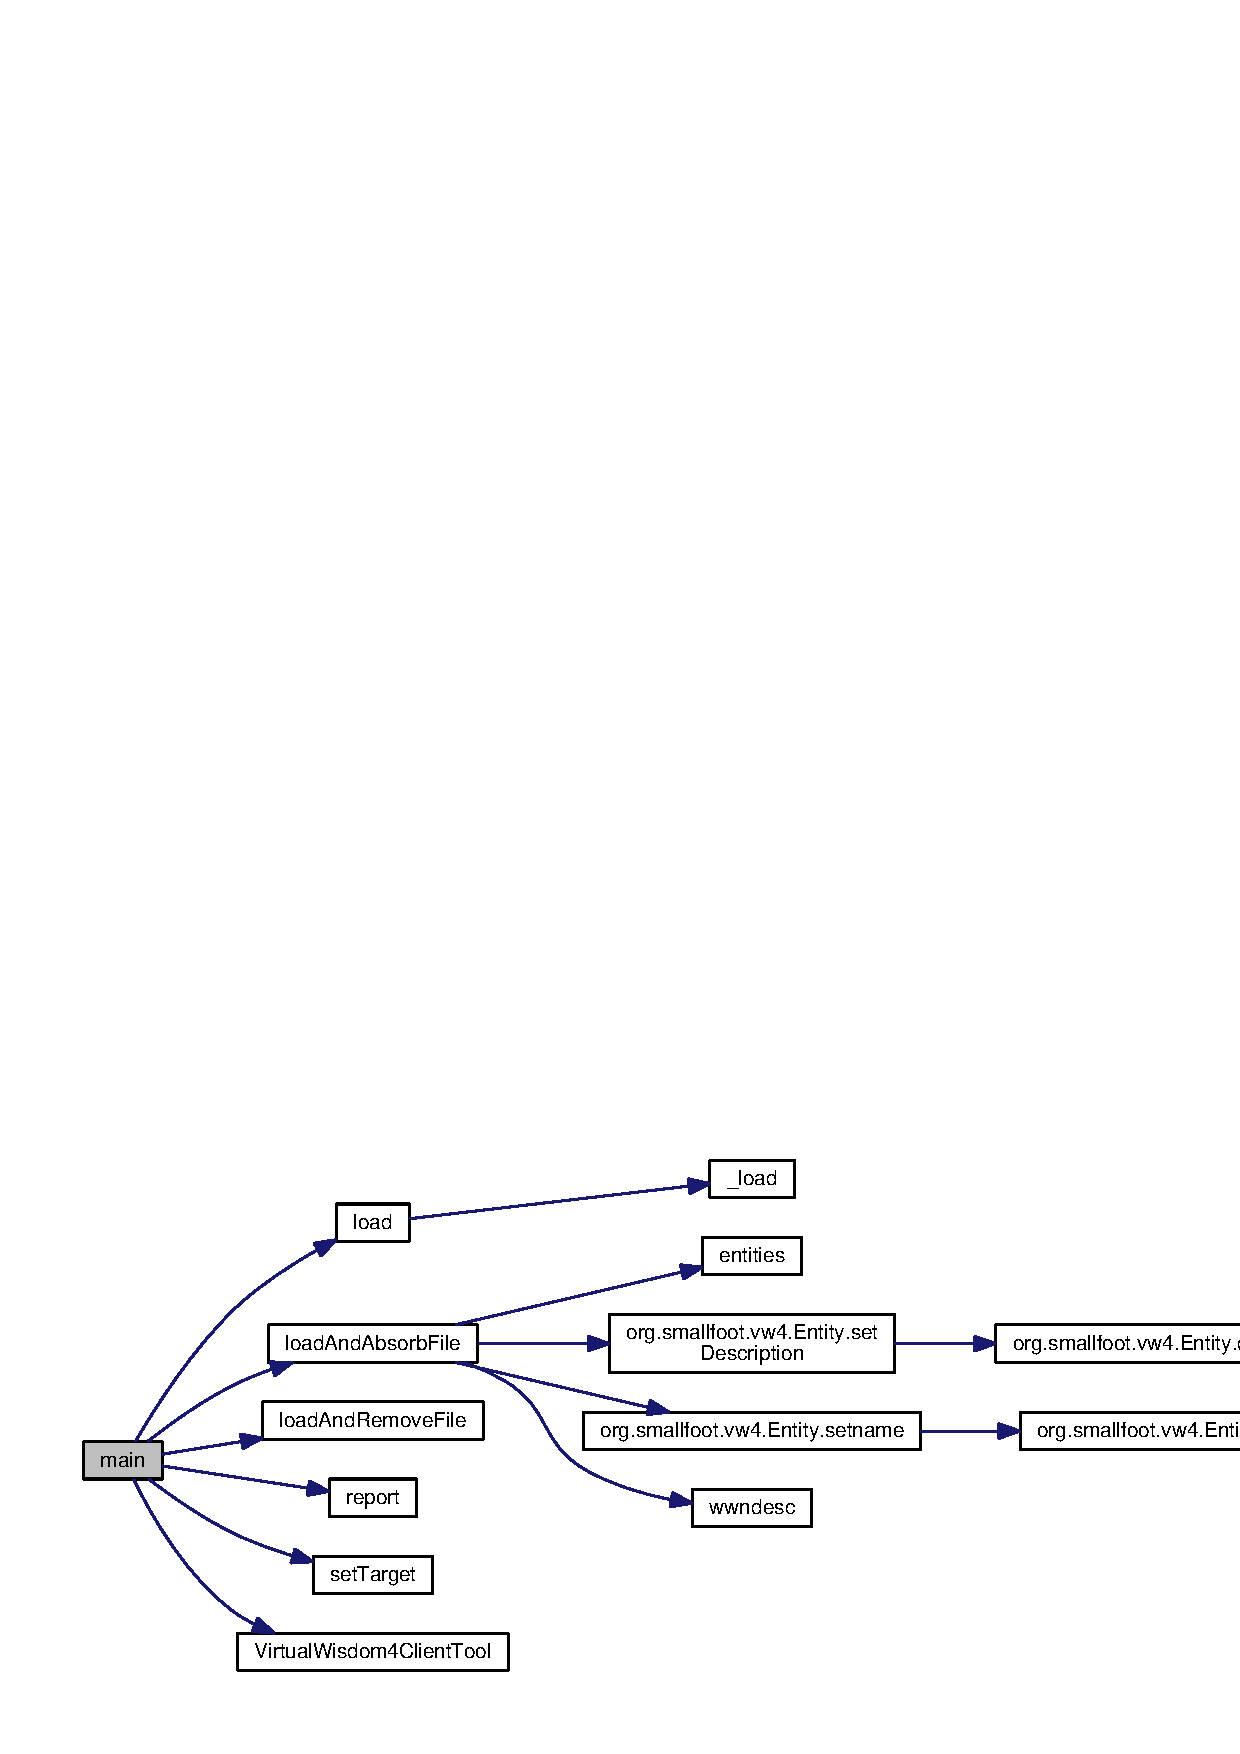
\includegraphics[width=350pt]{classorg_1_1smallfoot_1_1vw4_1_1VirtualWisdom4ClientTool_a75988cf84fc6ee7a2ebff36e363021aa_cgraph}
\end{center}
\end{figure}


\index{org\+::smallfoot\+::vw4\+::\+Virtual\+Wisdom4\+Client\+Tool@{org\+::smallfoot\+::vw4\+::\+Virtual\+Wisdom4\+Client\+Tool}!patterns@{patterns}}
\index{patterns@{patterns}!org\+::smallfoot\+::vw4\+::\+Virtual\+Wisdom4\+Client\+Tool@{org\+::smallfoot\+::vw4\+::\+Virtual\+Wisdom4\+Client\+Tool}}
\subsubsection[{patterns}]{\setlength{\rightskip}{0pt plus 5cm}Vector$<$Pattern$>$ patterns (
\begin{DoxyParamCaption}
{}
\end{DoxyParamCaption}
)\hspace{0.3cm}{\ttfamily [inline]}}\label{classorg_1_1smallfoot_1_1vw4_1_1VirtualWisdom4ClientTool_a09f298d19a33be899f5835657c747c5d}
$<$ singleton access for patterns \begin{DoxyReturn}{Returns}
collection of patterns 
\end{DoxyReturn}


Definition at line 187 of file Virtual\+Wisdom4\+Client\+Tool.\+java.

\index{org\+::smallfoot\+::vw4\+::\+Virtual\+Wisdom4\+Client\+Tool@{org\+::smallfoot\+::vw4\+::\+Virtual\+Wisdom4\+Client\+Tool}!pretty\+J\+S\+O\+N@{pretty\+J\+S\+O\+N}}
\index{pretty\+J\+S\+O\+N@{pretty\+J\+S\+O\+N}!org\+::smallfoot\+::vw4\+::\+Virtual\+Wisdom4\+Client\+Tool@{org\+::smallfoot\+::vw4\+::\+Virtual\+Wisdom4\+Client\+Tool}}
\subsubsection[{pretty\+J\+S\+O\+N}]{\setlength{\rightskip}{0pt plus 5cm}String pretty\+J\+S\+O\+N (
\begin{DoxyParamCaption}
\item[{V\+W\+Import}]{v}
\end{DoxyParamCaption}
)\hspace{0.3cm}{\ttfamily [inline]}}\label{classorg_1_1smallfoot_1_1vw4_1_1VirtualWisdom4ClientTool_afc3ee9b897e0757b6cd5c8289c9d4cc4}


Convenience function to generate a pretty-\/printed J\+S\+O\+N text string. 


\begin{DoxyParams}{Parameters}
{\em v} & V\+W\+Import object to markup \\
\hline
\end{DoxyParams}
\begin{DoxyReturn}{Returns}
a pretty-\/printed J\+S\+O\+N using Object\+Writer.\+with\+Default\+Pretty\+Printer() or null if an exception occurs 
\end{DoxyReturn}


Definition at line 161 of file Virtual\+Wisdom4\+Client\+Tool.\+java.

\index{org\+::smallfoot\+::vw4\+::\+Virtual\+Wisdom4\+Client\+Tool@{org\+::smallfoot\+::vw4\+::\+Virtual\+Wisdom4\+Client\+Tool}!save@{save}}
\index{save@{save}!org\+::smallfoot\+::vw4\+::\+Virtual\+Wisdom4\+Client\+Tool@{org\+::smallfoot\+::vw4\+::\+Virtual\+Wisdom4\+Client\+Tool}}
\subsubsection[{save}]{\setlength{\rightskip}{0pt plus 5cm}void save (
\begin{DoxyParamCaption}
\item[{String}]{filename}
\end{DoxyParamCaption}
)\hspace{0.3cm}{\ttfamily [inline]}}\label{classorg_1_1smallfoot_1_1vw4_1_1VirtualWisdom4ClientTool_a119573b242d96a5e64a7d340bcf14aa8}


Wrapper to just save the file, spitting out exceptions and stacks as they occur. 


\begin{DoxyParams}{Parameters}
{\em filename} & filename to save into \\
\hline
\end{DoxyParams}


Definition at line 142 of file Virtual\+Wisdom4\+Client\+Tool.\+java.



References Virtual\+Wisdom4\+Client\+Tool.\+\_\+save().



Here is the call graph for this function\+:\nopagebreak
\begin{figure}[H]
\begin{center}
\leavevmode
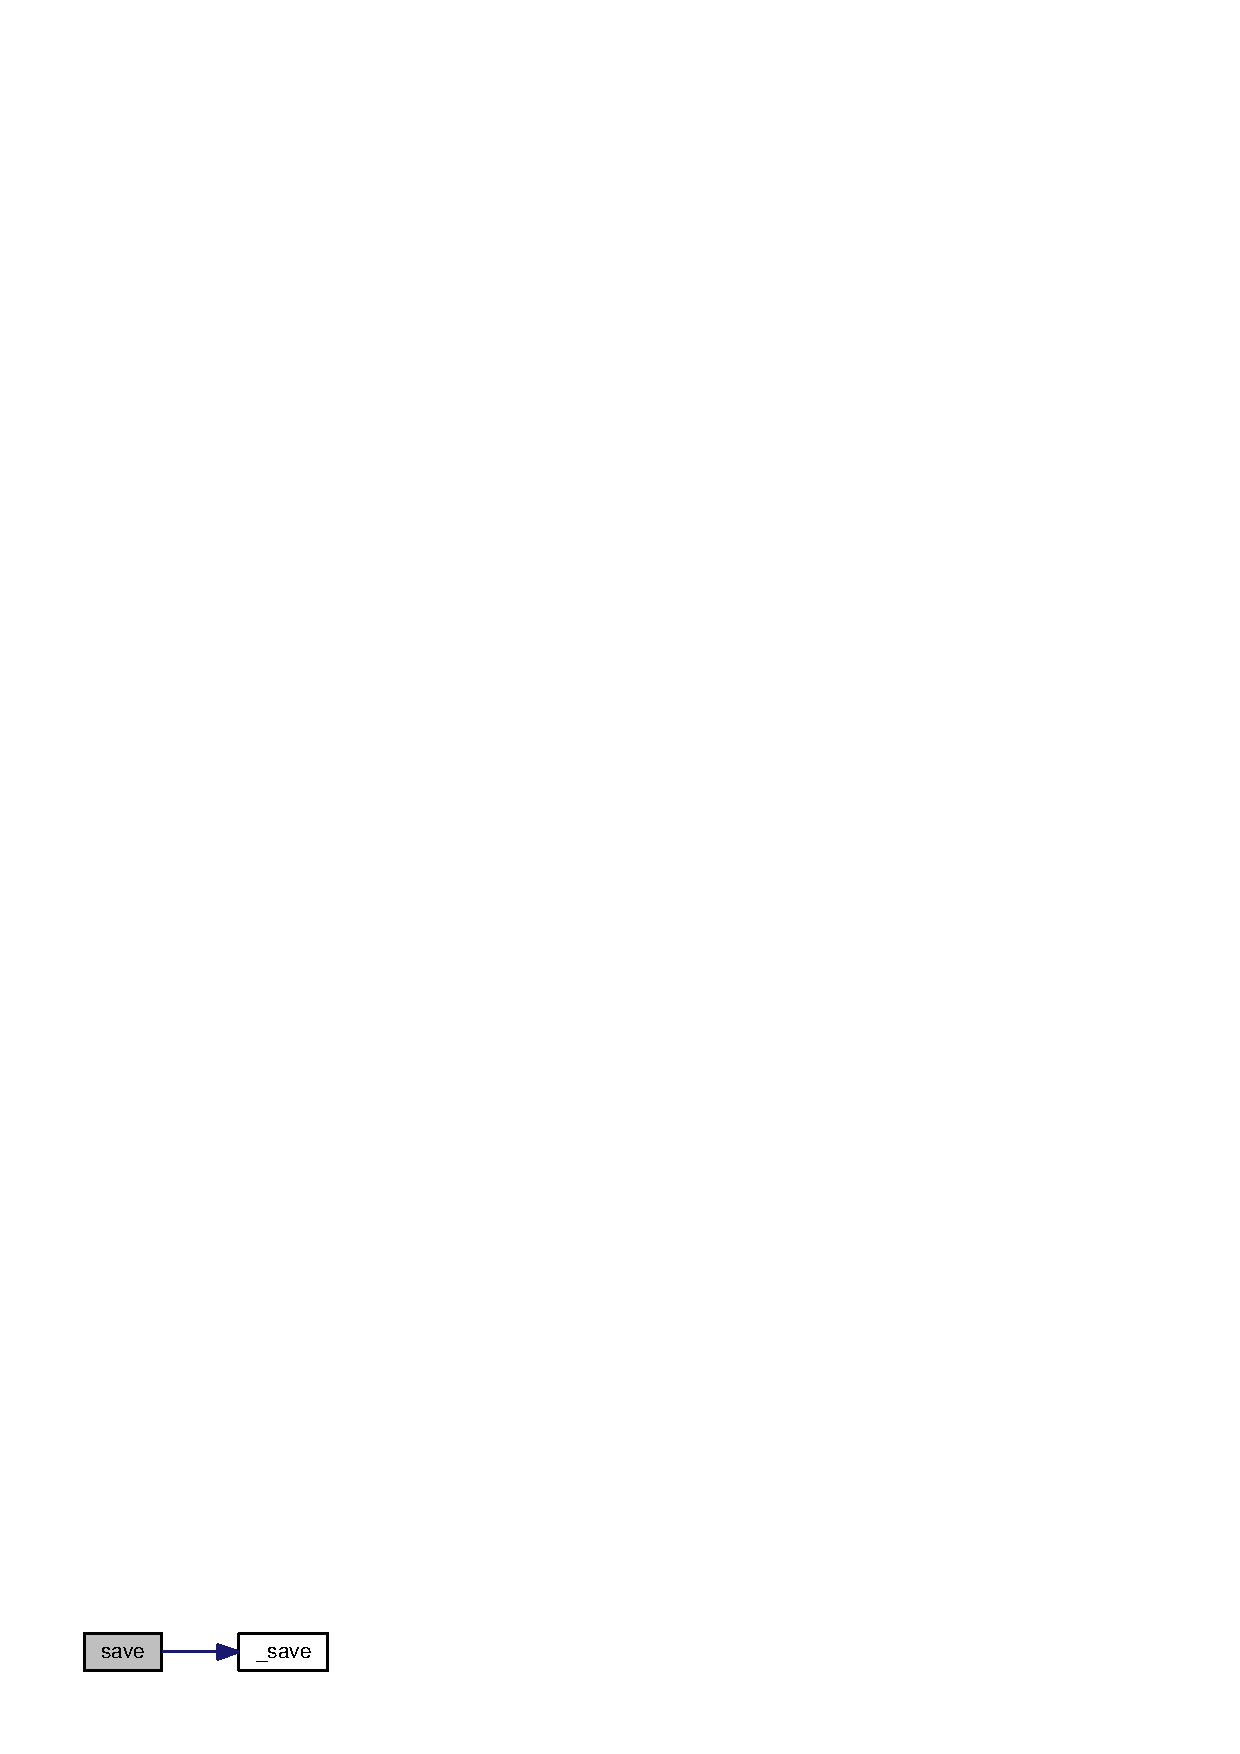
\includegraphics[width=162pt]{classorg_1_1smallfoot_1_1vw4_1_1VirtualWisdom4ClientTool_a119573b242d96a5e64a7d340bcf14aa8_cgraph}
\end{center}
\end{figure}


\index{org\+::smallfoot\+::vw4\+::\+Virtual\+Wisdom4\+Client\+Tool@{org\+::smallfoot\+::vw4\+::\+Virtual\+Wisdom4\+Client\+Tool}!vwimport@{vwimport}}
\index{vwimport@{vwimport}!org\+::smallfoot\+::vw4\+::\+Virtual\+Wisdom4\+Client\+Tool@{org\+::smallfoot\+::vw4\+::\+Virtual\+Wisdom4\+Client\+Tool}}
\subsubsection[{vwimport}]{\setlength{\rightskip}{0pt plus 5cm}V\+W\+Import vwimport (
\begin{DoxyParamCaption}
{}
\end{DoxyParamCaption}
)\hspace{0.3cm}{\ttfamily [inline]}, {\ttfamily [protected]}}\label{classorg_1_1smallfoot_1_1vw4_1_1VirtualWisdom4ClientTool_acbeee875159f78e186965708e70dee94}
$<$ singleton to access vwimport to allow for later post-\/process \begin{DoxyReturn}{Returns}
vwimport instance, created if needed 
\end{DoxyReturn}


Definition at line 82 of file Virtual\+Wisdom4\+Client\+Tool.\+java.



Referenced by Virtual\+Wisdom4\+Client\+Tool.\+main().

\index{org\+::smallfoot\+::vw4\+::\+Virtual\+Wisdom4\+Client\+Tool@{org\+::smallfoot\+::vw4\+::\+Virtual\+Wisdom4\+Client\+Tool}!wwndesc@{wwndesc}}
\index{wwndesc@{wwndesc}!org\+::smallfoot\+::vw4\+::\+Virtual\+Wisdom4\+Client\+Tool@{org\+::smallfoot\+::vw4\+::\+Virtual\+Wisdom4\+Client\+Tool}}
\subsubsection[{wwndesc}]{\setlength{\rightskip}{0pt plus 5cm}W\+W\+N\+Description wwndesc (
\begin{DoxyParamCaption}
{}
\end{DoxyParamCaption}
)\hspace{0.3cm}{\ttfamily [inline]}}\label{classorg_1_1smallfoot_1_1vw4_1_1VirtualWisdom4ClientTool_a43a8de962936ee9d82e0a70eeb9b1db6}
$<$ singleton access for wwndesc \begin{DoxyReturn}{Returns}
wwndesc 
\end{DoxyReturn}


Definition at line 201 of file Virtual\+Wisdom4\+Client\+Tool.\+java.



Referenced by Virtual\+Wisdom4\+Client\+Tool.\+load\+And\+Absorb\+File().



The documentation for this class was generated from the following file\+:\begin{DoxyCompactItemize}
\item 
java/{\bf Virtual\+Wisdom4\+Client\+Tool.\+java}\end{DoxyCompactItemize}

\chapter{File Documentation}
\section{java/\+Entity.java File Reference}
\label{Entity_8java}\index{java/\+Entity.\+java@{java/\+Entity.\+java}}
\subsection*{Data Structures}
\begin{DoxyCompactItemize}
\item 
class {\bf Entity}
\begin{DoxyCompactList}\small\item\em An \doxyref{Entity}{p.}{classorg_1_1smallfoot_1_1vw4_1_1Entity} is the core mutable object used in the J\+S\+O\+N import for V\+W4. \end{DoxyCompactList}\item 
class {\bf Entity.\+Improper\+Child\+Exception}
\begin{DoxyCompactList}\small\item\em Descendents of \doxyref{Entity}{p.}{classorg_1_1smallfoot_1_1vw4_1_1Entity} should know whether a given entity can be one of their child elements. \end{DoxyCompactList}\end{DoxyCompactItemize}

\section{java/\+Entity\+Array.java File Reference}
\label{EntityArray_8java}\index{java/\+Entity\+Array.\+java@{java/\+Entity\+Array.\+java}}
\subsection*{Data Structures}
\begin{DoxyCompactItemize}
\item 
class {\bf Entity\+Array}
\begin{DoxyCompactList}\small\item\em An \doxyref{Entity\+Array}{p.}{classorg_1_1smallfoot_1_1vw4_1_1EntityArray} is the representation of an Array entity in the J\+S\+O\+N import for V\+W4. \end{DoxyCompactList}\end{DoxyCompactItemize}

\section{java/\-Entity\-F\-A.java File Reference}
\label{EntityFA_8java}\index{java/\-Entity\-F\-A.\-java@{java/\-Entity\-F\-A.\-java}}
\subsection*{Data Structures}
\begin{DoxyCompactItemize}
\item 
class {\bf Entity\-F\-A}
\begin{DoxyCompactList}\small\item\em An \doxyref{Entity\-F\-A}{p.}{classorg_1_1smallfoot_1_1vw4_1_1EntityFA} is the representation of an Storage F\-A entity in the J\-S\-O\-N import for V\-W4. \end{DoxyCompactList}\end{DoxyCompactItemize}

\section{java/\+Entity\+H\+B\+A.java File Reference}
\label{EntityHBA_8java}\index{java/\+Entity\+H\+B\+A.\+java@{java/\+Entity\+H\+B\+A.\+java}}
\subsection*{Data Structures}
\begin{DoxyCompactItemize}
\item 
class {\bf Entity\+H\+B\+A}
\begin{DoxyCompactList}\small\item\em An \doxyref{Entity\+H\+B\+A}{p.}{classorg_1_1smallfoot_1_1vw4_1_1EntityHBA} is the representation of an H\+B\+A entity in the J\+S\+O\+N import for V\+W4. \end{DoxyCompactList}\end{DoxyCompactItemize}

\section{java/\+Entity\+Host.java File Reference}
\label{EntityHost_8java}\index{java/\+Entity\+Host.\+java@{java/\+Entity\+Host.\+java}}
\subsection*{Data Structures}
\begin{DoxyCompactItemize}
\item 
class {\bf Entity\+Host}
\begin{DoxyCompactList}\small\item\em An \doxyref{Entity\+Host}{p.}{classorg_1_1smallfoot_1_1vw4_1_1EntityHost} is the representation of an Host entity in the J\+S\+O\+N import for V\+W4. \end{DoxyCompactList}\end{DoxyCompactItemize}

\section{java/\-Virtual\-Wisdom4\-Client\-Tool.java File Reference}
\label{VirtualWisdom4ClientTool_8java}\index{java/\-Virtual\-Wisdom4\-Client\-Tool.\-java@{java/\-Virtual\-Wisdom4\-Client\-Tool.\-java}}
\subsection*{Data Structures}
\begin{DoxyCompactItemize}
\item 
class {\bf Virtual\-Wisdom4\-Client\-Tool}
\begin{DoxyCompactList}\small\item\em \doxyref{Virtual\-Wisdom4\-Client\-Tool}{p.}{classorg_1_1smallfoot_1_1vw4_1_1VirtualWisdom4ClientTool} is a \char`\"{}\-Swiss Army Knife\char`\"{} of tools used when working with Virtual\-Wisdom4. \end{DoxyCompactList}\end{DoxyCompactItemize}

\section{java/\-V\-W\-Import.java File Reference}
\label{VWImport_8java}\index{java/\-V\-W\-Import.\-java@{java/\-V\-W\-Import.\-java}}
\subsection*{Data Structures}
\begin{DoxyCompactItemize}
\item 
enum {\bf V\-W\-Import.\-Edit\-\_\-\-Type}
\begin{DoxyCompactList}\small\item\em The edit type of a J\-S\-O\-N for V\-W4 Import can be either \char`\"{}add\char`\"{} or \char`\"{}modify\char`\"{}; the creator needs to know ahead of time whether an entry of the same name currently exists. \end{DoxyCompactList}\item 
class {\bf V\-W\-Import.\-Entity}
\begin{DoxyCompactList}\small\item\em An entity for import. \end{DoxyCompactList}\item 
class {\bf V\-W\-Import.\-I\-T\-L\-Pattern}
\begin{DoxyCompactList}\small\item\em An \doxyref{I\-T\-L\-Pattern}{p.}{classorg_1_1smallfoot_1_1vw4_1_1VWImport_1_1ITLPattern} is udes to define an application \doxyref{Entity}{p.}{classorg_1_1smallfoot_1_1vw4_1_1VWImport_1_1Entity} based on the I\-T\-Ls it requires. \end{DoxyCompactList}\item 
class {\bf V\-W\-Import}
\begin{DoxyCompactList}\small\item\em A \doxyref{V\-W\-Import}{p.}{classorg_1_1smallfoot_1_1vw4_1_1VWImport} is a single idempotent import for the Virtual\-Wisdom4 product. \end{DoxyCompactList}\end{DoxyCompactItemize}

\section{scripts/csv-\/to-\/json.awk File Reference}
\label{csv-to-json_8awk}\index{scripts/csv-\/to-\/json.\+awk@{scripts/csv-\/to-\/json.\+awk}}

%--- End generated contents ---

% Index
\newpage
\phantomsection
\addcontentsline{toc}{chapter}{Index}
\printindex

\end{document}
